\chapter{Controlling the ROV} \label{cha:controller} \index{Open-Loop Control} \index{Controller} \index{Exact Linearisation}
Automatic control is way of regulating a process without direct human interaction. This can range from approximately decoupling a dynamic system via a decoupling matrix to advanced more advanced controllers. There are two main concepts of control, open-loop and feedback control. Open-loop control is a controller that computes its output based on a model of the system and sometimes the current states. \Figureref{fig:control_system_open} illustrates the open-loop control scheme used in the \abbrROV. Feedback control is a controller that uses the error of the direct measurement or estimated state minus the reference value \textit{i.e.} 
\begin{equation}
e = \hat{x} - x_{\text{ref}}
\end{equation}
to control. The control scheme for the \abbrROV can be seen in \Figureref{fig:control_system}. A feedback controller can as the open-loop control use a model of the system. Using the model in the control structure can produce better performance and remove unwanted effects such as non-linearities, this is wanted due to the fact that a lot of control principles are based on linear systems \citep{reglerteori}. 

\begin{figure}
	\centering
		\begin{tikzpicture}[auto, thick, node distance=2cm,>=latex',
			 block/.style  = {draw, rectangle,minimum height=3em, minimum width=6em},
			 sum/.style    = {draw, circle, inner sep=0pt, text width=4mm,align=center, node distance=1cm},
			 input/.style  = {coordinate},
			 output/.style = {coordinate},
			 pinstyle/.style = {pin edge={to-,thin,black}}]
			 
		    \node [input, name=input] {};
		    \node [block, right of=input, node distance=3cm] (controller) {F};
		    \node [block, right of=controller, node distance=3cm] (system) {\abbrROV};
		
		    \draw [->] (controller) -- node[name=u] {$u$} (system);
		    \node [output, right of=system] (output) {};
		
		    \draw [draw,->] (input) -- node {$u_{\text{control}}$} (controller);
		    \draw [->] (system) -- node [name=y] {$y$}(output);
		\end{tikzpicture}
	\caption{The open-loop control scheme used in the \abbrROV. The control block F can be any type of open-loop control. Notice that this is an ideal case were no disturbances affect the system.}
	\label{fig:control_system_open}
\end{figure}

\begin{figure}
	\centering
		\begin{tikzpicture}[auto, thick, node distance=2cm,>=latex',
			 block/.style  = {draw, rectangle,minimum height=3em, minimum width=6em},
			 sum/.style    = {draw, circle, inner sep=0pt, text width=4mm,align=center, node distance=1cm},
			 input/.style  = {coordinate},
			 output/.style = {coordinate},
			 pinstyle/.style = {pin edge={to-,thin,black}}]
			 
		    \node [input, name=input] {};
		    \node [sum, right of=input] (sum) {+};
		    \node [block, right of=sum] (controller) {F};
		    \node [block, right of=controller, node distance=3cm] (system) {\abbrROV};
		
		    \draw [->] (controller) -- node[name=u] {$u$} (system);
		    \node [output, right of=system] (output) {};
		    \node [block, below of=u] (sensorfusion) {Observer};
		
		    \draw [draw,->] (input) -- node {$x_{\text{ref}}$} (sum);
		    \draw [->] (sum) -- node {$e$} (controller);
		    \draw [->] (system) -- node [name=y] {$y$}(output);
		    \draw [->] (y) |- (sensorfusion);
		    \draw [->] (sensorfusion) -| node[pos=0.99] {$-$} 
		        node [near end] {$\hat{x}$} (sum);
		\end{tikzpicture}
	\caption{The feedback control scheme used in the \abbrROV. The controller F can be any of the controllers discussed in this chapter. The observer in the \abbrROV is the sensor fusion described in \Chapterref{cha:sensor_fusion}. Notice that this is an ideal case were no disturbances affect the system.}
	\label{fig:control_system}
\end{figure}

Exact linearisation is when the dynamics of the system are compensated by a non-linear control signal and thus can linear control principles be used \citep{reglerteori}. Using the model structure from \Chapterref{cha:modelling} and the estimated parameters from \Chapterref{cha:parameterEstimation} the exact linearisation for the \abbrROV  is defined as
\begin{equation}
f^{-1}(\etaVector,\nuVector) = \inertia \accVector^{\text{b}} + \damping(\nuVector) + \coriolis(\nuVector) + \gravity(\etaVector)
\end{equation}
where $\accVector^b$ is the commanded angular acceleration in the body-fixed frame \citep[p.451]{fossen2011}.
\todo[inline]{Write some control theory. Exact lin... Background}
%%%%%%%%%%%%%%%%%%%%%%%%%%%%%%%%%%%%%%%
\section{Open-Loop Control} \label{sec:openloop} \index{Open-Loop Control} \index{thrust allocation} \index{thruster geometry}
The open loop control of the \abbrROV consists of an static thrust allocation matrix which is
\begin{equation}
    \thrusterGeometryOnes[*] = \thrusterGeometryOnes[T](\thrusterGeometryOnes \thrusterGeometryOnes[T])^{-1}
\end{equation}
where $\thrusterGeometryOnes$ describes how the actuators effect the \abbrROV \citep{thrustallocation}. The thrust geometry matrix $\thrusterGeometryOnes$ has been derived from the thrust matrix $\thrusterGeometry$ and became 
\begin{equation*}
    \thrusterGeometryOnes = 
    \begin{bmatrix}
    0  & 0  & 1 & 1  &  0 &  0 \\
    0  & 0  & 0 & 0  &  0 & -1 \\
    -1 & -1 & 0 & 0  & -1 &  0 \\
    1  & -1 & 0 & 0  &  0 &  0 \\
    1  & 1  & 0 & 0  & -1 &  0 \\
    0  & 0  & 1 & -1 &  0 &  0 \\
    \end{bmatrix}
\end{equation*}
and thus $\thrusterGeometryOnes[*]$ is given by
\begin{equation}
\thrusterGeometryOnes= \begin{bmatrix}
0 & 0 & -0.25 & 0.5 & 0.25 & 0 \\
0 & 0 & -0.25 & -0.5 & 0.25 & 0 \\
0.5 & 0 & 0 & 0 & 0 & 0.5 \\
0.5 & 0 & 0 & 0 & 0 & -0.5 \\
0 & 0 & -0.5 & 0 & -0.5 & 0 \\
0 & -1 & 0 & 0 & 0 & 0 \\
\end{bmatrix}
\end{equation}
The static thrust allocation matrix $\thrusterGeometryOnes[*]$ is the pseudo inverse of the thrust geometry matrix $\thrusterGeometryOnes$. An approximately decoupled control is achieved when the static thrust allocation matrix is used and thus can the \abbrROV be controlled better without using any controllers. \Figureref{fig:open_control} illustrates how the control signals are allocated to the different thrusters when given an control input.

\begin{figure}
    \centering
    \begin{tikzpicture}[auto, thick, node distance=3cm, >=latex',%
        block/.style    = {draw, thick, rectangle, minimum height = 3em,%
        minimum width = 3em},%
      sum/.style      = {draw, circle, node distance = 2cm},% 
      input/.style    = {coordinate},%
      output/.style   = {coordinate} %
    ]
    \draw
    	% Drawing the blocks of first filter :
    	node at (0,0)[input, name=input1] (input1) {}
    	node [block, right of=input1] (inte1) {\thrusterGeometryOnes[*]}
    	node [output, right of=inte1] (output1) {};
        % Joining blocks. 
        % Commands \draw with options like [->] must be written individually
    	\draw[->](input1) -- node {$u_{\text{control}}$}(inte1);
     	\draw[->](inte1) -- node {$u$} (output1);
    \end{tikzpicture}
    \caption{The open-loop control allocate control signals by the thrust allocation matrix $\thrusterGeometryOnes[*]$. The static thrust allocation matrix gives an approximately decoupled control.}
    \label{fig:open_control}
\end{figure}

%%%%%%%%%%%%%%%%%%%%%%%%%%%%%%%%%%%%%%%%
\section{Attitude Controller} \index{PID@\abbrPID!abbreviation} \index{Attitude Controller}
\todo[inline]{Write some fluff}
Using the relations in \Chapterref{cha:modelling} the derivative of the attitude error can be defined as 
\begin{equation}
\etaTildeAngdot = \dot{\boldsymbol{T}}_\theta(\eulerAngles)\nuVectorAng
\end{equation}
and the attitude error can be defined as 
\begin{equation}
\etaTildeAng = \etaVectorAng - \etaVectorAng[,_{\text{ref}}] 
\end{equation}
This gives the \abbrPID attitude controller
\begin{equation}
	\accVector^b = \begin{bmatrix} 
	\zeroCol{3} \\
	\boldsymbol{T}^{-1}_\theta(\eulerAngles)(-K_{\text{p}} \etaTildeAng - K_{\text{i}}\int \! \etaTildeAng \, \mathrm{d}t - K_{\text{d}} \etaTildeAngdot - \dot{\boldsymbol{T}}_\theta(\eulerAngles) \etaVectorAng)
	\end{bmatrix}
\end{equation}
where $K_{\text{p}}$, $K_{\text{i}}$ and $K_{\text{d}}$ are positive definite design matrices \citep[p. 453]{fossen2011}. 
Using the open-loop control of the linear velocities with exact linearisation of the attitude controller gives
\begin{equation}
	u_{\etaVectorAng} = f^{-1}(\etaVector,\nuVector) + \thrusterGeometryOnes[*] \begin{bmatrix} \nuVectorLin \\ \zeroCol{3} \end{bmatrix}
\end{equation}
or
\begin{equation}
	u_{\etaVectorAng} = \accVector^b + \thrusterGeometryOnes[*] \begin{bmatrix} \nuVectorLin \\ \zeroCol{3} \end{bmatrix}
\end{equation}
without the exact linearisation. An illustration of how the attitude controller with open-loop control is implemented can be seen in \Figureref{fig:attitudecontroller}.

\begin{figure}
	\centering
	\begin{tikzpicture}[auto, thick, node distance=2cm, >=latex',%
        block/.style  = {draw, thick, rectangle, minimum height = 1cm,%
                           minimum width = 3em},%
        PID/.style    = {draw, thick, rectangle, minimum height = 1cm,%
                         minimum width = 0.6cm},%
        sum/.style    = {draw, circle,inner sep=0pt, text width=4mm,align=center,node distance = 1cm},%
        mux/.style    = {draw, thick, rectangle, minimum width=0.3cm,%
                        minimum height = 2cm ,fill= black!100,%
                        node distance=1cm},
        input/.style    = {coordinate},%
        output/.style   = {coordinate} %
    ]
   		\draw node at (0,0) [input] (vel_input) {};
   		\draw node [input,below of=vel_input] (ang_input) {};
   		\draw node[PID, right of=ang_input] (pid) {$\abbrPID$};
   		
   		%from input to pid
   		\draw[->] (ang_input) -- node[align=center, below] {$\etaVectorAng - \etaVectorAng[,\text{ref}]$} ($(pid.west)$);
   		\draw (pid.east) -- ++(0.5,0) node[](switch){};
   		
   		%from pid to switch and making the switch 
   		\draw (pid.east) ++(2,0.5) node[](switchup){};
   		\draw (pid.east) ++(2,-0.5) node[block, name=exactlin] {$f^{-1}(\etaVector,\nuVector)$};
   		\draw (pid.east) ++(0.8,0.5) -| (switchup);
   		\draw (pid.east) ++(0.8,-0.5) -| (exactlin.west);
   		\draw (pid.east) ++(0.5,0) -- ++(0.3,0.5);
   		\draw[->] (pid.east) ++(0.65,0.25) arc (30:-30:0.6);     		
   		
   		%Merge the switch  		
   		\draw (pid.east) ++(3,0) node[coordinate](merge){};
   		\draw (switchup) -| (merge);
   		\draw (exactlin) -| (merge);
   		
   		%Input to thrust
   		\draw node[block, right of=vel_input] (thrust) {$\thrusterGeometryOnes[*]$};
   		\draw[->] (vel_input) -- node[align=center, below] {$\nuVectorLin[,\text{ref}]$} (thrust.west);
   		
   		%To sum
   		\draw (thrust.east) ++(4,0) node[sum, name=sum] {$+$};
		\draw[->] (thrust.east) -- node[align=center, below] {$u_{\nuVectorLin}$} (sum.west);
   		\draw[->] (merge) -| node[align=center, below] {$u_{\etaVectorAng}$} (sum.south);   		   		
   		% From sum to output
   		\draw node [output, right of=sum, node distance=2cm] (output) {};
    		\draw[->] (sum.east) -- node[align=center, below] {$u$} (output);	
	\end{tikzpicture}
    \caption{The linear velocities are controlled in the same way as in \Sectionref{sec:openloop}. However, the attitude are controlled via an \abbrPID and exact linearisation can be enabled.} 
    \label{fig:attitudecontroller}
\end{figure}

%%%%%%%%%%%%%%%%%%%%%%%%%%%%%%%%%%%%%%%%
\section{Angular Velocities Controller} \index{Angular Velocities Controller} \index{PI@\abbrPI!abbreviation}
\todo[inline]{Write some fluff about the rate controller}

If the angular velocities error are defined as 
\begin{equation}
\nuTildeAng = \nuVectorAng - \nuVectorAng[,_{\text{ref}}]
\end{equation}
then are the \abbrPI angular velocities controller defined as 
\begin{equation}
	\accVector^b = \begin{bmatrix} 
	\zeroCol{3} \\
	\boldsymbol{T}^{-1}_\theta(\eulerAngles)(-K_{\text{p}}*\nuTildeAng - K_{\text{i}}\int \! \nuTildeAng \, \mathrm{d}t)
	\end{bmatrix}
\end{equation}
where $K_{\text{p}}$ and $K_{\text{i}}^b$ are positive definite design matrices \citep[p. 453]{fossen2011}.
Using the exact linearisation for the angular velocities controller and open-loop control for the linear velocities, are the control signals defined as
\begin{equation}
	u_{\etaVectorAng} = f^{-1}(\etaVector,\nuVector) + \thrusterGeometryOnes[*] \begin{bmatrix} \nuVectorLin \\ \zeroCol{3} \end{bmatrix}	
\end{equation}
or the control signals can be defined as 
\begin{equation}
	u_{\etaVectorAng} = \accVector^b + \thrusterGeometryOnes[*] \begin{bmatrix} \nuVectorLin \\ \zeroCol{3} \end{bmatrix}
\end{equation}
if the exact linearisation is not wanted. \Figureref{fig:ratecontroller} illustrates how the angular velocities controller is implemented with the open-loop control of the linear velocities.
\begin{figure}
	\centering
	\begin{tikzpicture}[auto, thick, node distance=2cm, >=latex',%
        block/.style  = {draw, thick, rectangle, minimum height = 1cm,%
                           minimum width = 3em},%
        PID/.style    = {draw, thick, rectangle, minimum height = 1cm,%
                         minimum width = 0.6cm},%
        sum/.style    = {draw, circle,inner sep=0pt, text width=4mm,align=center,node distance = 1cm},%
        mux/.style    = {draw, thick, rectangle, minimum width=0.3cm,%
                        minimum height = 2cm ,fill= black!100,%
                        node distance=1cm},
        input/.style    = {coordinate},%
        output/.style   = {coordinate} %
    ]
   		\draw node at (0,0) [input] (vel_input) {};
   		\draw node [input,below of=vel_input] (ang_input) {};
   		\draw node[PID, right of=ang_input] (pid) {$\abbrPI$};
   		
   		%from input to pid
   		\draw[->] (ang_input) -- node[align=center, below] {$\nuVectorAng - \nuVectorAng[,\text{ref}]$} ($(pid.west)$);
   		\draw (pid.east) -- ++(0.5,0) node[](switch){};
   		
   		%from pid to switch and making the switch 
   		\draw (pid.east) ++(2,0.5) node[](switchup){};
   		\draw (pid.east) ++(2,-0.5) node[block, name=exactlin] {$f^{-1}(\etaVector,\nuVector)$};
   		\draw (pid.east) ++(0.8,0.5) -| (switchup);
   		\draw (pid.east) ++(0.8,-0.5) -| (exactlin.west);
   		\draw (pid.east) ++(0.5,0) -- ++(0.3,0.5);
   		\draw[->] (pid.east) ++(0.65,0.25) arc (30:-30:0.6);     		
   		
   		%Merge the switch  		
   		\draw (pid.east) ++(3,0) node[coordinate](merge){};
   		\draw (switchup) -| (merge);
   		\draw (exactlin) -| (merge);
   		
   		%Input to thrust
   		\draw node[block, right of=vel_input] (thrust) {$\thrusterGeometryOnes[*]$};
   		\draw[->] (vel_input) -- node[align=center, below] {$\nuVectorLin[,\text{ref}]$} (thrust.west);
   		
   		%To sum
   		\draw (thrust.east) ++(4,0) node[sum, name=sum] {$+$};
		\draw[->] (thrust.east) -- node[align=center, below] {$u_{\nuVectorLin}$} (sum.west);
   		\draw[->] (merge) -| node[align=center, below] {$u_{\nuVectorAng}$} (sum.south);   		   		
   		% From sum to output
   		\draw node [output, right of=sum, node distance=2cm] (output) {};
    		\draw[->] (sum.east) -- node[align=center, below] {$u$} (output);
	\end{tikzpicture}
    \caption{The linear velocities are controlled in the same way as in \Sectionref{sec:openloop}. However, the angular velocities are controlled via an \abbrPID and exact linearisation can be enabled.} 
    \label{fig:ratecontroller}
\end{figure}

%%%%%%%%%%%%%%%%%%%%%%%%%%%%%%%%%%%%%%%%
\section{Depth Controller} \index{Depth Controller} \index{PI@\abbrPI!abbreviation}
\todo[inline]{write some fluff} 
If the error in $\zPosition$ is defined as 
\begin{equation}
\tilde{\zPosition} = \zPosition - \zPosition_{\text{ref}}
\end{equation}
then is the \abbrPI depth controller defined as
\begin{equation}
u = \thrusterGeometryOnes[*]\begin{bmatrix} \boldsymbol{R}^n_b(\eulerAngles)^T \begin{bmatrix}
0 \\
0 \\
- K_{\text{p}} \tilde{\zPosition} - K_{\text{i}}\int \! \tilde{\zPosition} \, \mathrm{d}t
\end{bmatrix} \\ \zeroCol{3}\end{bmatrix}
\end{equation}
where $K_{\text{p}}$ and $K_{\text{i}}$ are design parameters. The rotation matrix $\boldsymbol{R}^n_b(\eulerAngles)^T$ is used to make the depth controller control the depth regardless the attitude of the \abbrROV. As can be seen in \Figureref{fig:depthcontroller} the depth controller can be used even if any of the other controllers are used. This is because the depth controller only adds or subtracts control signal to those thrusters that affect the depth.

\begin{figure}
	\centering
	\begin{tikzpicture}[auto, thick, node distance=2cm, >=latex',%
        block/.style  = {draw, thick, rectangle, minimum height = 1cm,%
                           minimum width = 3em},%
        PID/.style    = {draw, thick, rectangle, minimum height = 1cm,%
                         minimum width = 0.6cm},%
        sum/.style    = {draw, circle,inner sep=0pt, text width=4mm,align=center,node distance = 1cm},%
        mux/.style    = {draw, thick, rectangle, minimum width=0.3cm,%
                        minimum height = 2cm ,fill= black!100,%
                        node distance=1cm},
        input/.style    = {coordinate},%
        output/.style   = {coordinate} %
    ]
   		\draw node at (0,0) [input] (vel_input) {};
		\draw node[input, below of=vel_input] (ang_input) {};
   		\draw node[PID, right of=ang_input] (pid) {$\abbrPI$};
   		
   		%from input to pid
   		\draw[->] (ang_input) -- node[align=center, below] {$\zPosition - \zPosition_{\text{ref}}$} ($(pid.west)$);
   		\draw (pid.east) -- ++(0.5,0) node[](switch){};
   		
   		%from pid to switch and making the switch 
   		\draw (pid.east) ++(2,0) node[coordinate](switchup){};
  		\draw (pid.east) ++(1.2,0) -- (switchup);
   		\draw (pid.east) ++(0.5,0) -- ++(0.3,0.5);
   		\draw[->] (pid.east) ++(0.65,0.25) arc (30:0:0.6);     		
   		
   		%Merge the switch  		
   		\draw (pid.east) ++(3,0) node[coordinate](merge){};
   		\draw (switchup) -- (merge);
   		
   		%Input to thrust
   		\draw node[block, right of=vel_input] (controller) {F};
   		\draw[->] (vel_input) -- node[align=center, below] {$x_{\text{ref}}$} (controller.west);
   		
   		%To sum
   		\draw (controller.east) ++(4,0) node[sum, name=sum] {$+$};
		\draw[->] (controller.east) -- (sum.west);
   		\draw[->] (merge) -| node[align=center, below] {$u_{\zPosition}$}  (sum.south);   		   		
   		% From sum to output
   		\draw node [output, right of=sum, node distance=2cm] (output) {};
    		\draw[->] (sum.east) -- node[align=center, below] {$u$} (output);
	\end{tikzpicture}
    \caption{The \abbrPI depth controller can be used when the open-loop control is engaged or when the other controllers are used. In this figure the F symbolises the chosen way of controlling the \abbrROV.} 
    \label{fig:depthcontroller}
\end{figure}

%%%%%%%%%%%%%%%%%%%%%%%%%%%%%%%%%%%%%%%%
\section{Benchmarking}
To be able to draw any conclusions about the performance of the controllers the following reference signals was used
\begin{description}
\item[Constant] A constant reference was applied to all \abbrDOF. This reference signal was only used for trimming the controllers initially, thus will no results be presented expect for the depth controller.

\item[Sine] A $\sin(\cdot)$ signal was applied to one \abbrDOF at the time and then to all \abbrDOF. Two $\sin$ signals with different amplitudes were used, amplitude $1$ and $0.5$. The used frequency was $0.5 \hertz$.

\item[Smooth step] A smooth step was applied to one \abbrDOF at the time and then to all \abbrDOF at the same time. The used smooth step was the same as in \citet[p. 192-195]{robotics}. The smooth step parameters were $q_{\text{0}} = 0$, $q_{\text{f}} = 1$, $t_{\text{s}} = 3$ ,$t_{\text{f}} = 15$ and $V = 1.5 (q_{\text{f}} - q_{\text{0}})/(t_{\text{f}} - t_{\text{s}}))$
\end{description}
for each controller separately. For each conducted test was there a simulated test except for the depth because the depth dynamics has not been modelled. The \abbrROV model in the simulator used the parameters from \Sectionref{sec:parameterResults}. The exact linearisation, both in the simulator and the \abbrROV, used the parameters from \Sectionref{sec:parameterResults} with an scaling factor of 0.9 except for $z_B$ which had 0.5 as scaling factor. In this Section will a few representative test cases will be presented,  several other test can be seen in \Appref{app:controllerTestResults}. Tests was conducted for the \abbrPID attitude controller without exact linearisation, the \abbrPI rate controller with exact linearisation and with the \abbrPI depth controller. The parameters used in the \abbrPID and the \abbrPI:s during simulation and real tests can be seen in \Tableref{tab:parametersAttitude} - \Tableref{tab:parametersDepth}. Different performance evaluation values will be used, these values are defined as in \citet{reglerteori}. 

\begin{table}[tbp]
  \centering
  \caption{\label{tab:parametersAttitude}%
    The parameters used in the attitude controller's \abbrPID.}
  \begin{tabular}{l l l l}
    \toprule%
       & \textbf{$K_\text{p}$} & \textbf{$K_\text{i}$}& \textbf{$K_\text{d}$}\\
    \otoprule%   
    $\rollAngle$  & 2   & 0.1 & 0.1 \\
    $\pitchAngle$ & 2.7 & 0.1 & 0.1 \\
    $\yawAngle$   & 0.7 & 0.1 & 0.1 \\
    \bottomrule%
  \end{tabular}
\end{table}

\begin{table}[tbp]
  \centering
  \caption{\label{tab:parametersRate}%
    The parameters used in the rate controller's \abbrPI.}
  \begin{tabular}{l l l}
    \toprule%
       & \textbf{$K_\text{p}$} & \textbf{$K_\text{i}$}\\
    \otoprule%   
    $\rollVelocity$  & 3.5 & 2 \\
    $\pitchVelocity$ & 3.5 & 2 \\
    $\yawVelocity$   & 3.0 & 2 \\
    \bottomrule%
  \end{tabular}
\end{table}

\begin{table}[tbp]
  \centering
  \caption{\label{tab:parametersDepth}%
    The parameters used in the depth controller's \abbrPI.}
  \begin{tabular}{l l l}
    \toprule%
       & \textbf{$K_\text{p}$} & \textbf{$K_\text{i}$}\\
    \otoprule%   
    $\zPosition$  & 1 & 0.2 \\
    \bottomrule%
  \end{tabular}
\end{table}

\begin{figure}
\centering
  \subfloat[][\label{fig:testExactAttitudeRoll} The exact linearisation in $\rollAngle$.]{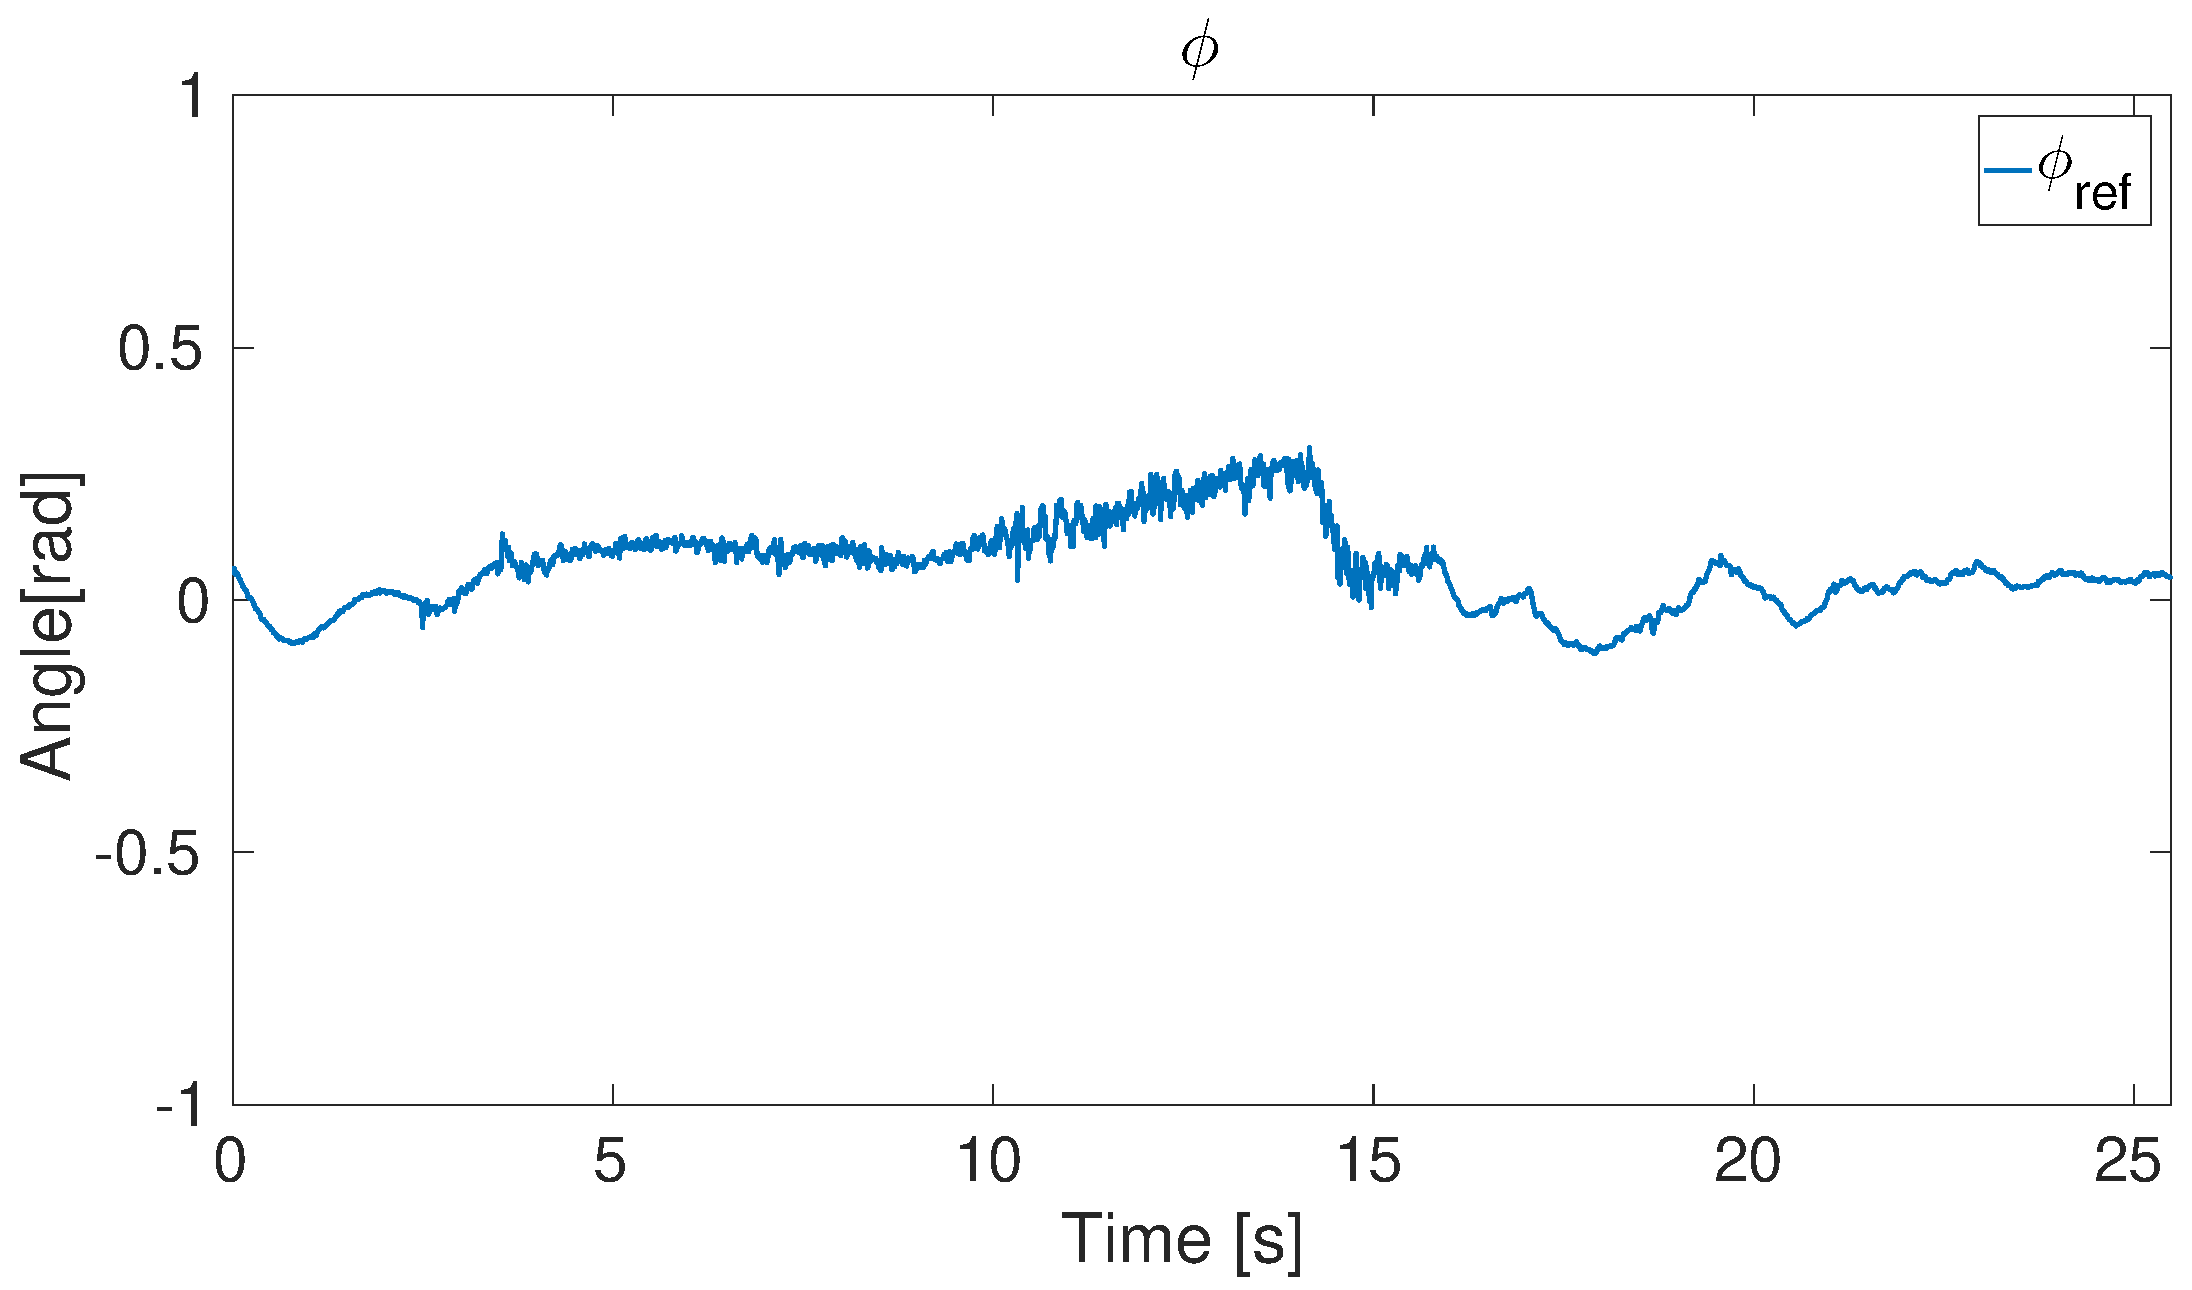
\includegraphics[width=0.4\textwidth]{testExactLinAttitudePhi}}
  \qquad
  \subfloat[][\label{fig:testExactAttitudePitch} The exact linearisation in $\pitchAngle$.]{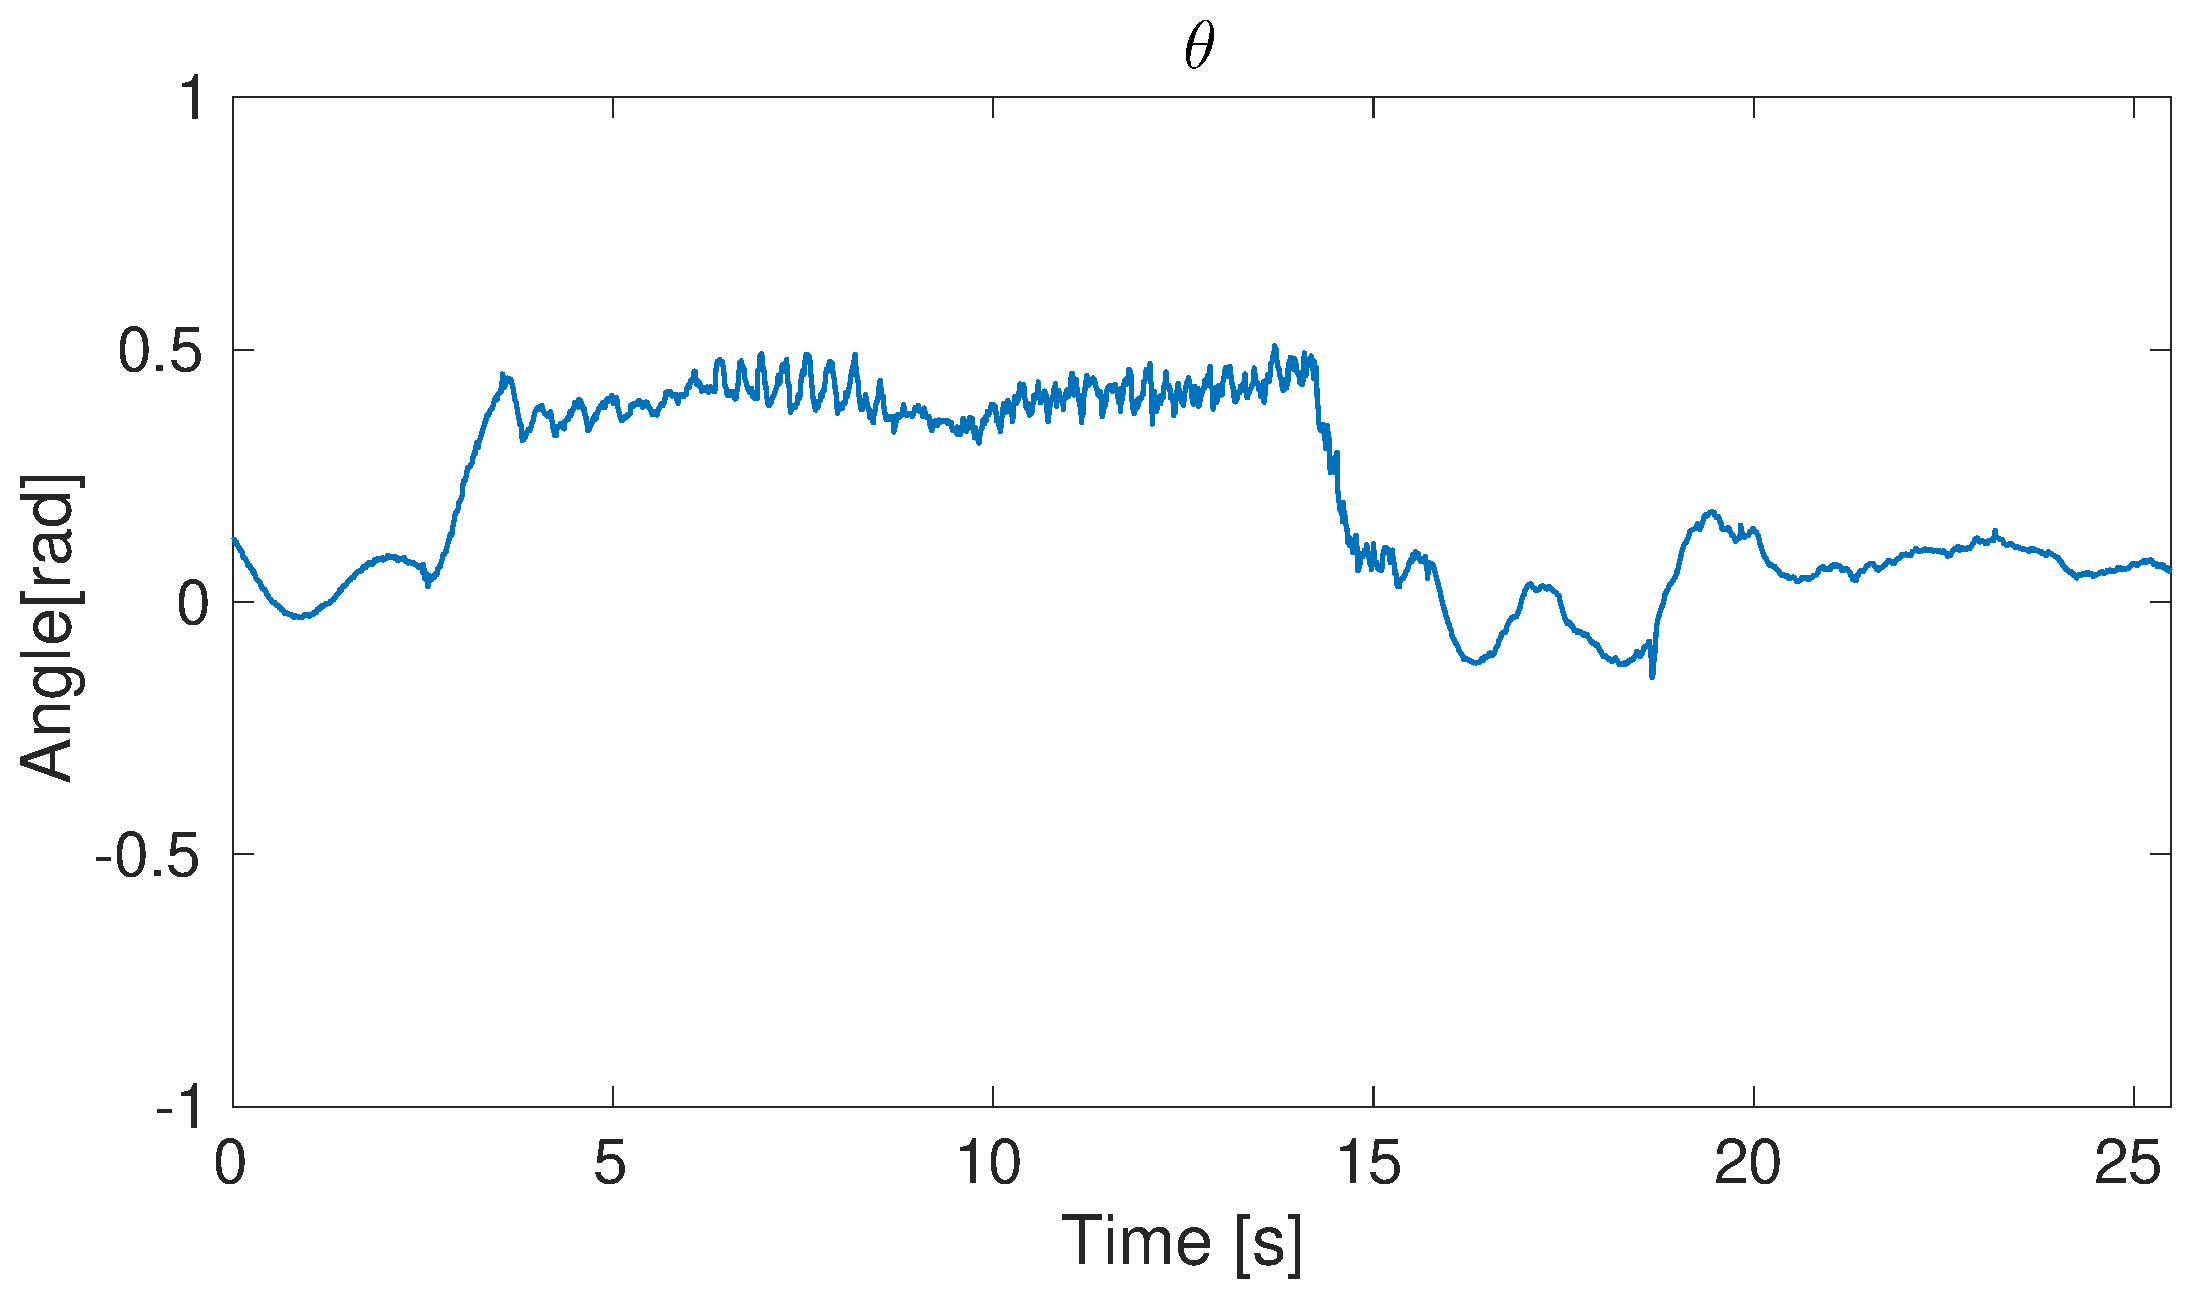
\includegraphics[width=0.4\textwidth]{testExactLinAttitudeTheta}}
  \qquad
  \subfloat[][\label{fig:testExactAttitudeYaw} The exact linearisation in $\yawAngle$.]{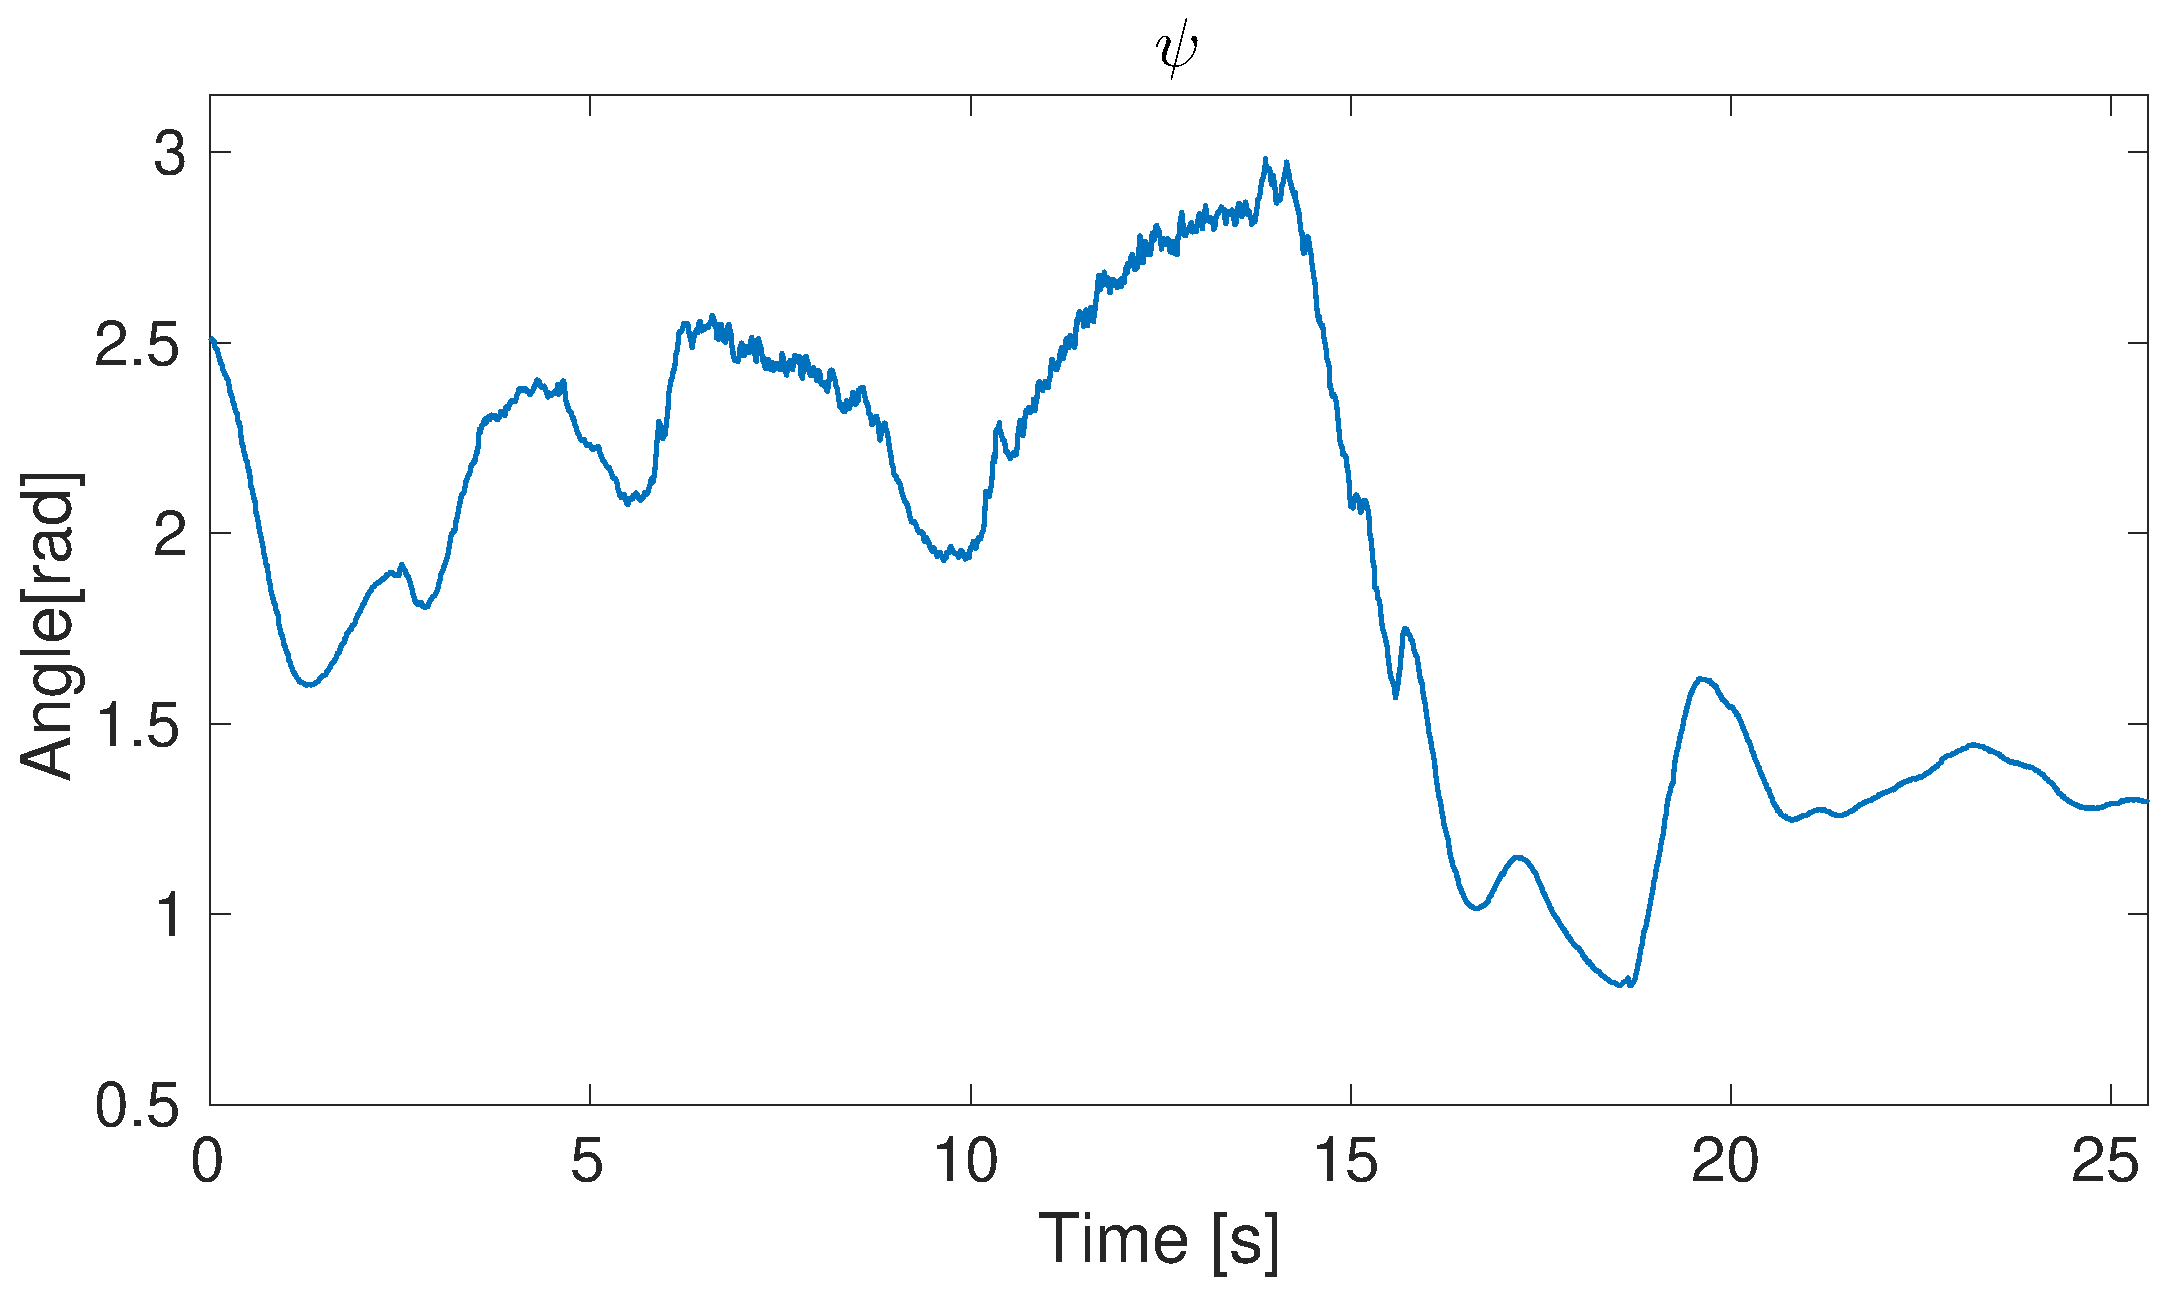
\includegraphics[width=0.4\textwidth]{testExactLinAttitudePsi}}
  \caption{\label{fig:ExactLinAttitude}% 
  The exact linearisation in the attitude controller. No reference signal was sent during this test thus is it only the effect of the exact linearisation showing.}
\end{figure}

\Figureref{fig:ExactLinAttitude} shows the exact linearisation in the attitude controller. Even that no reference signals are given begins the \abbrROV to change attitude.  
%%%%%%%%%%%%%%%%%%%%%%%%%%%Attitude%%%%%%%%%%%%%%%%%

\begin{figure}
\centering
  \subfloat[][\label{fig:testStepAllRollAttitude} A smooth step applied in $\rollAngle$.]{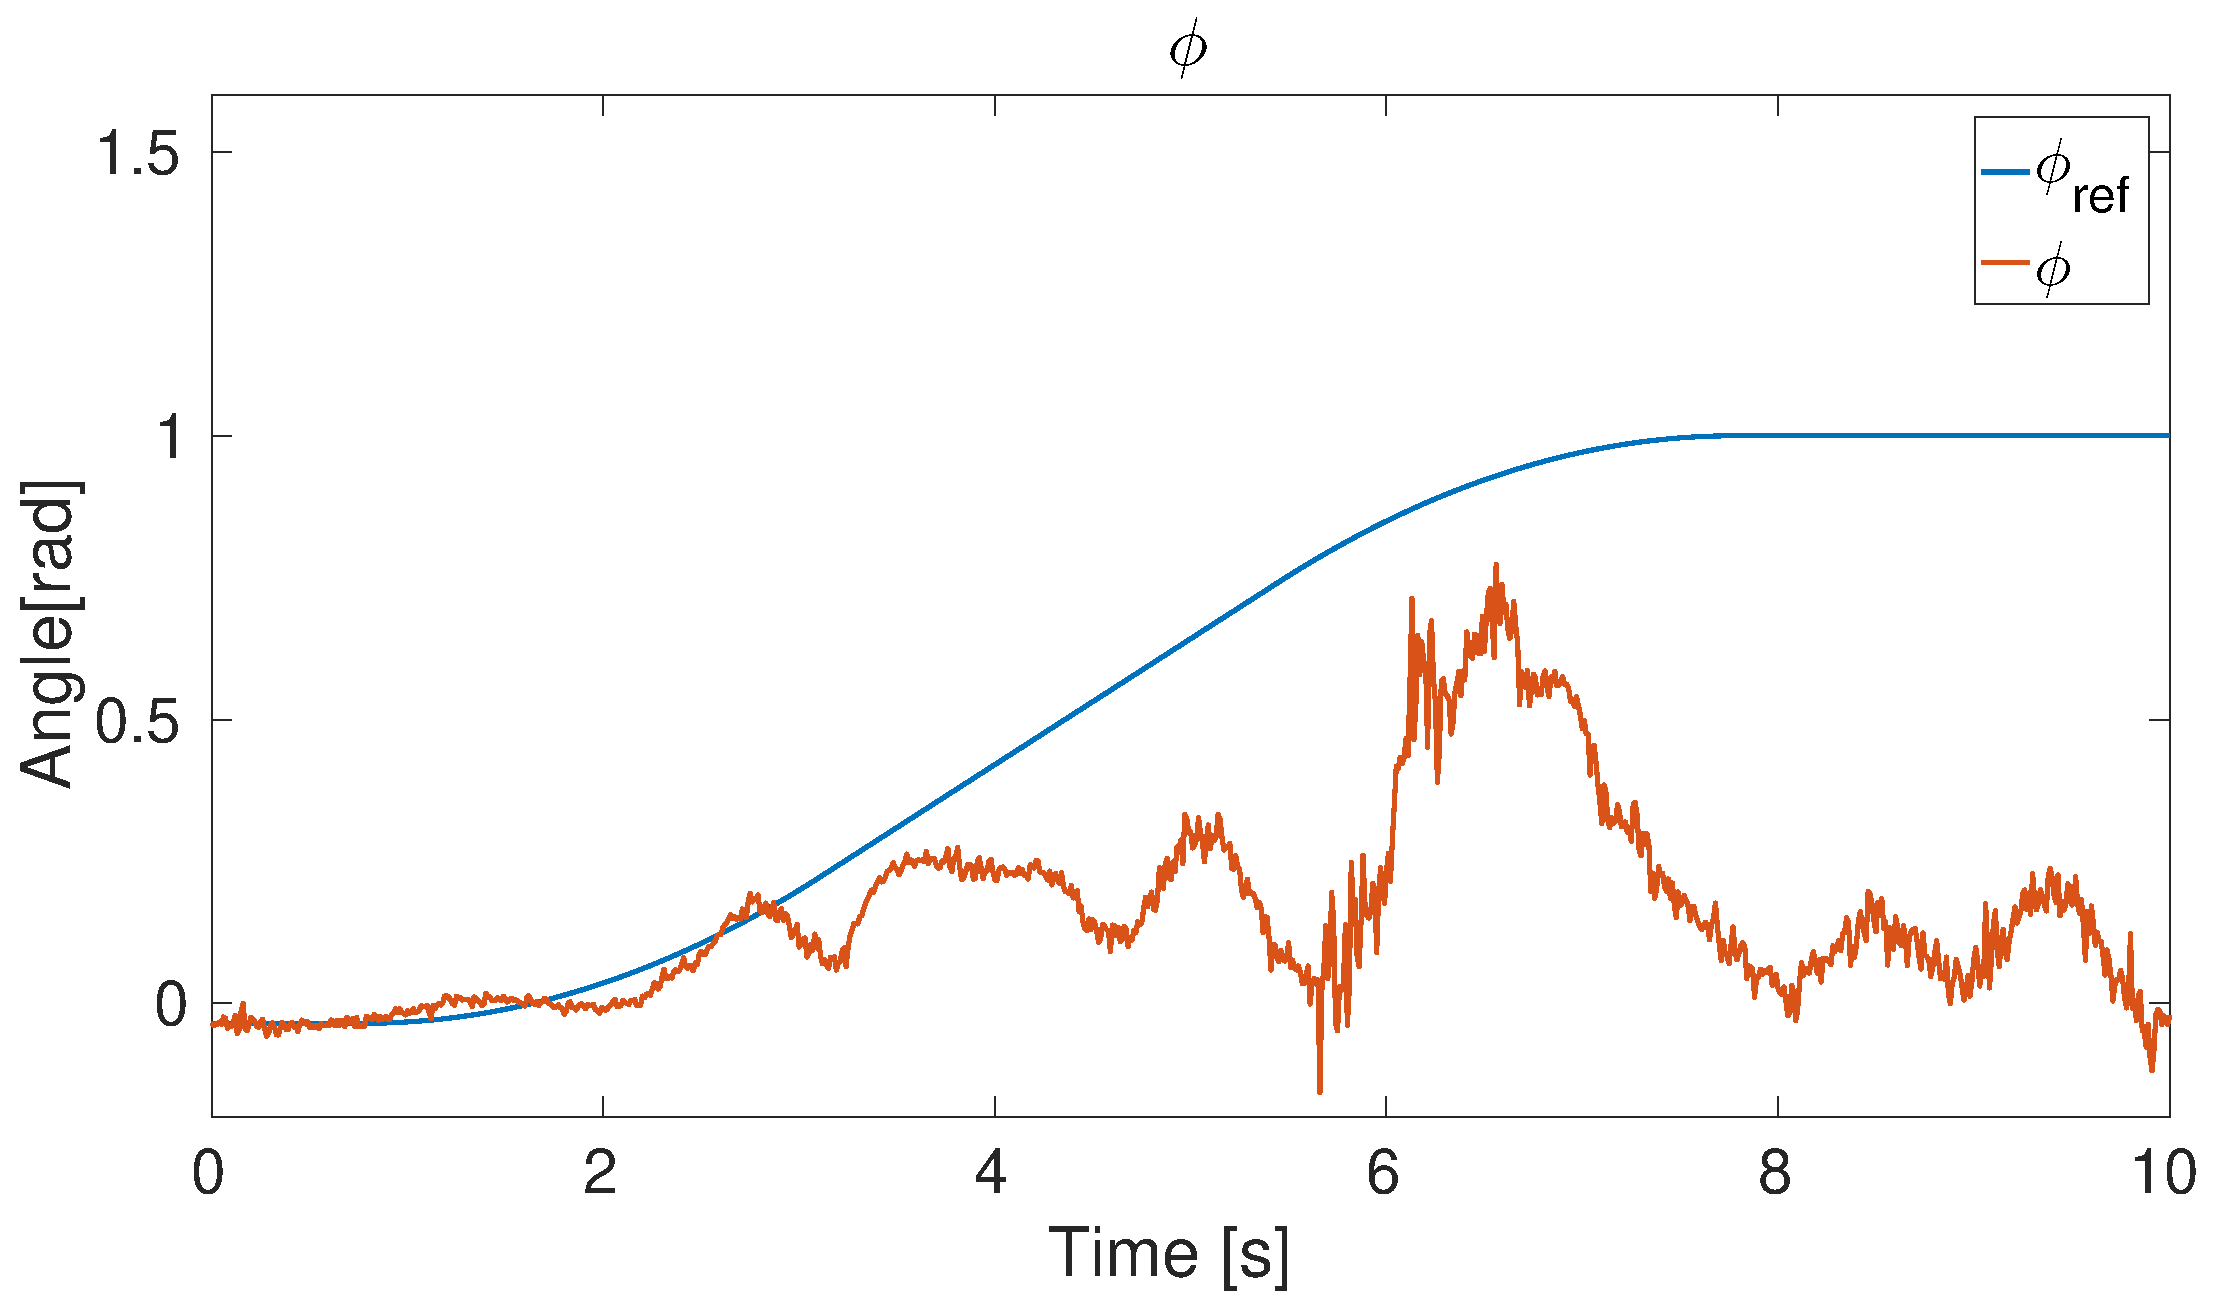
\includegraphics[width=0.4\textwidth]{testStepAllPhis3e10a1}}
  \qquad
  \subfloat[][\label{fig:simStepAllRollAttitude} A smooth step applied to the simulated \abbrROV in $\rollAngle$.]{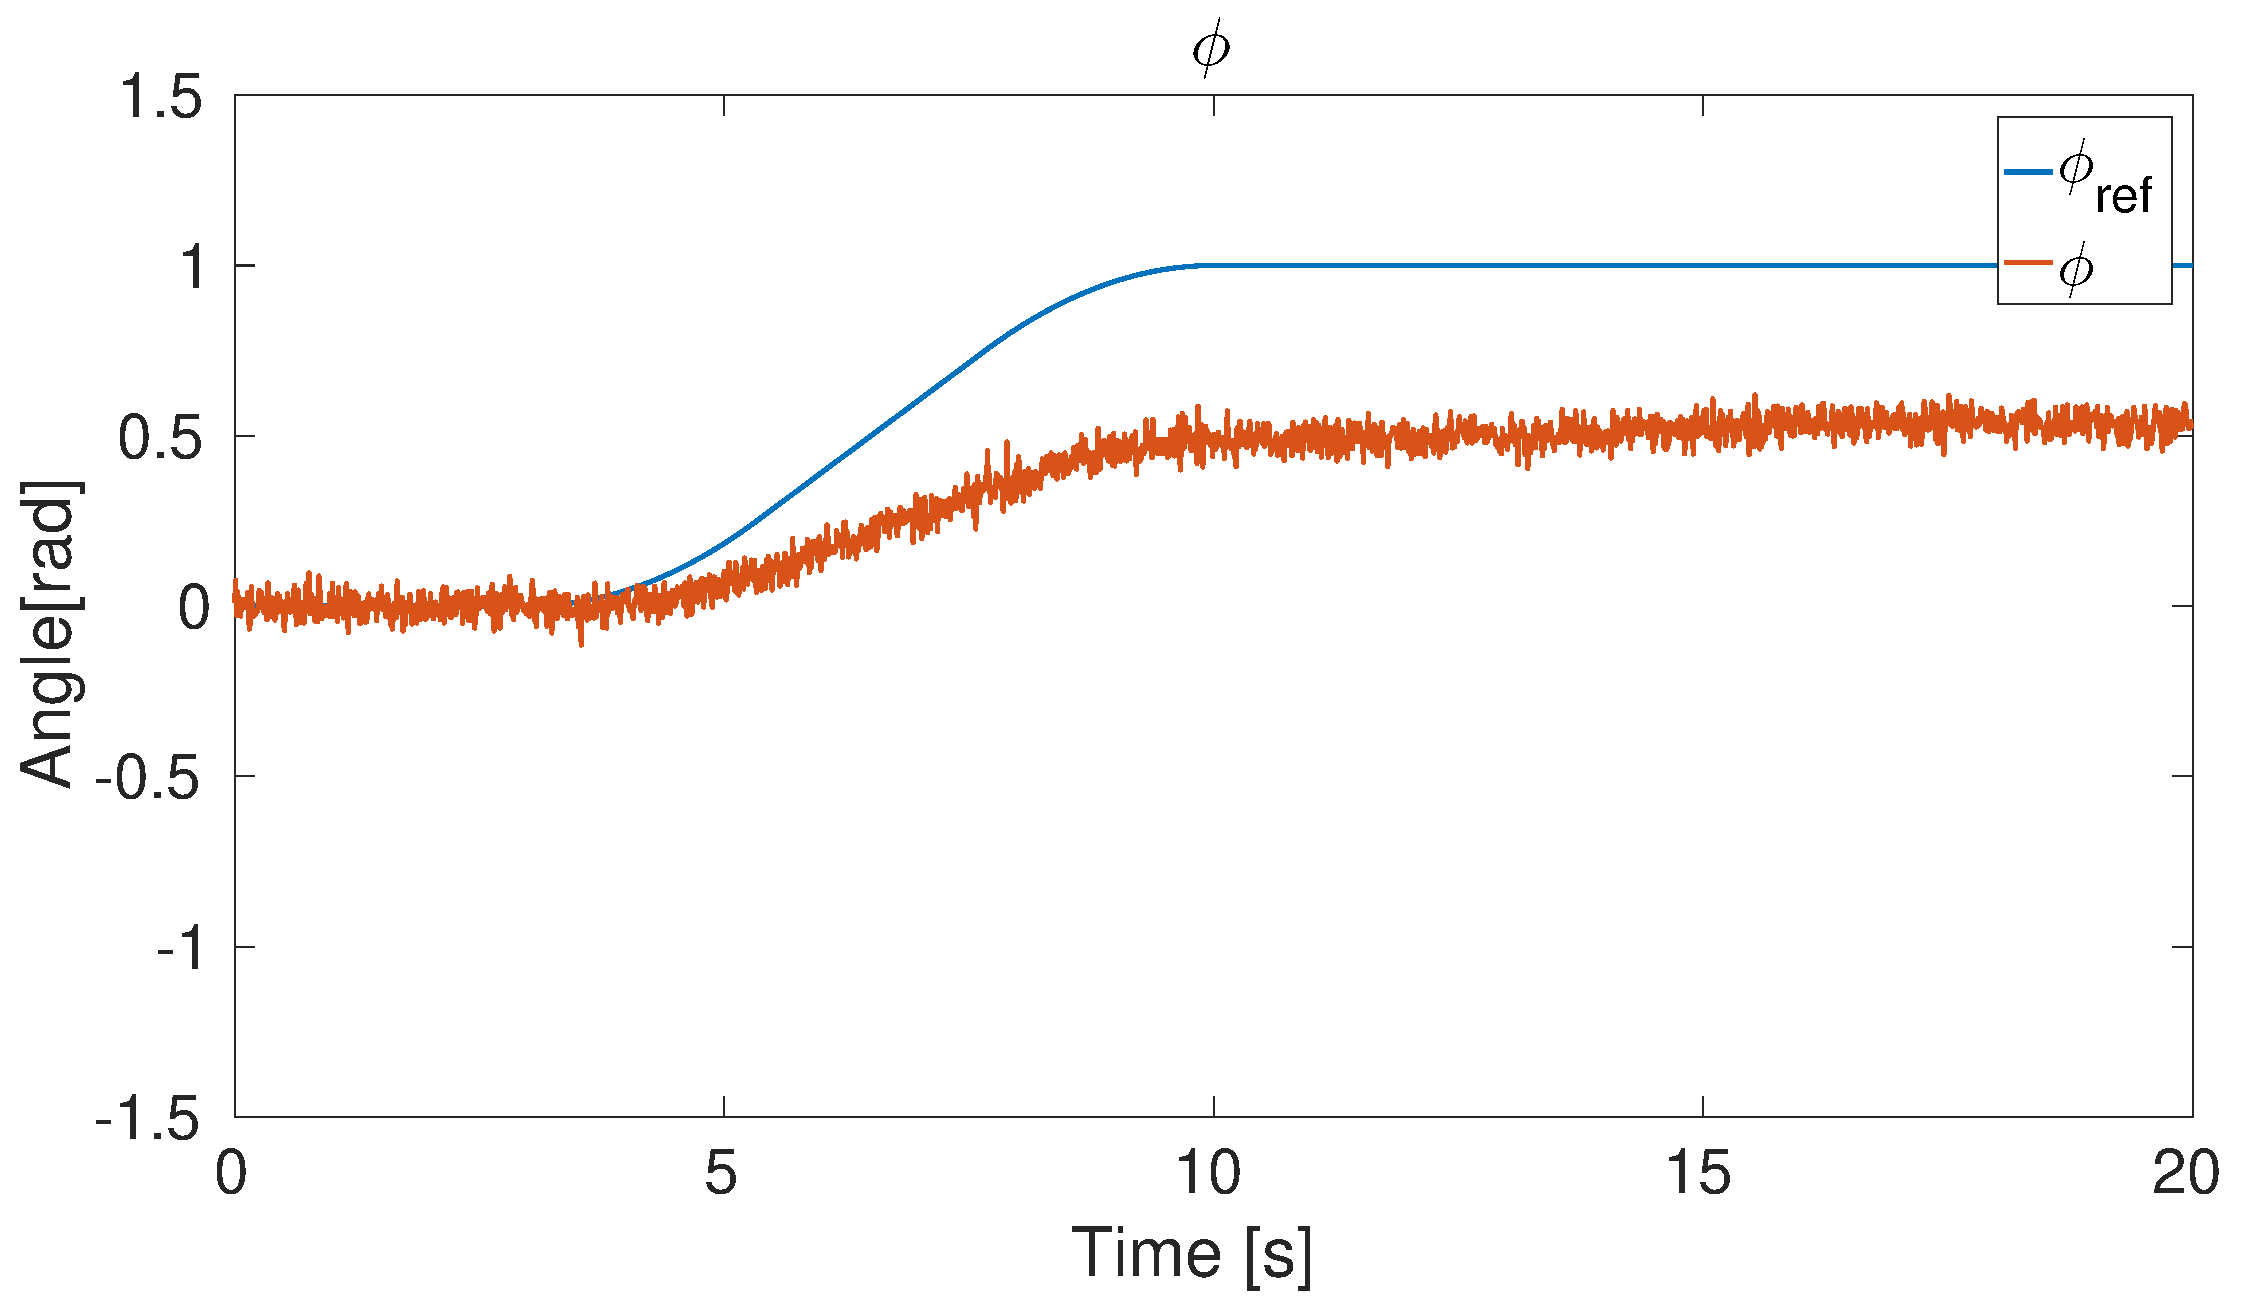
\includegraphics[width=0.4\textwidth]{simStepAllPhis3e10a1}}
  \qquad
  \subfloat[][\label{fig:TestStepAllPitchAttitude} A smooth step applied in $\pitchAngle$.]{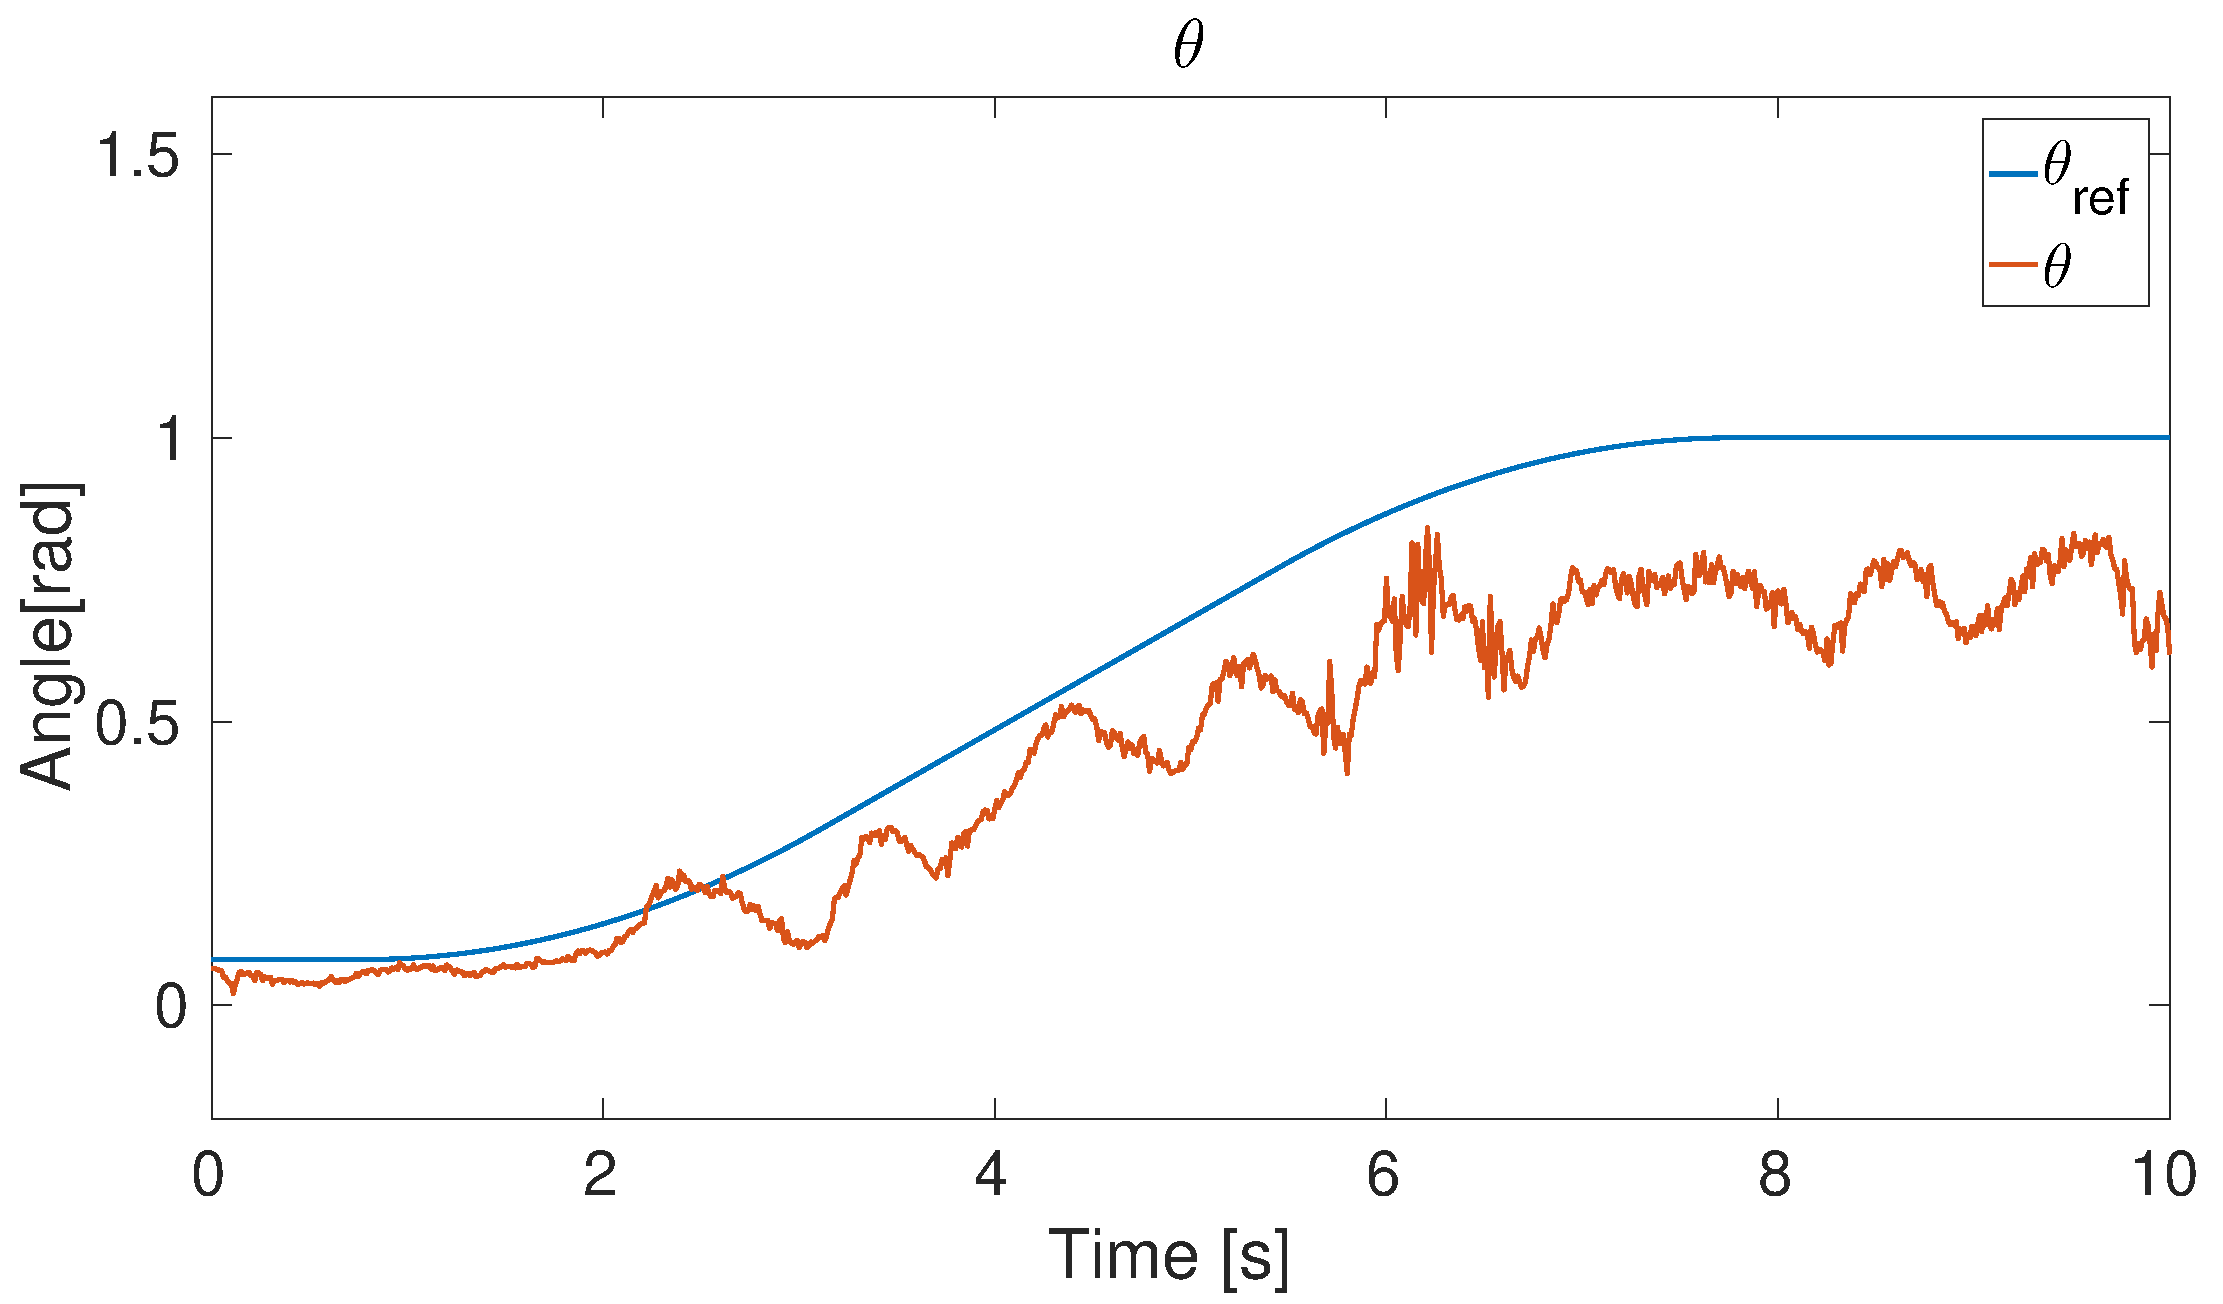
\includegraphics[width=0.4\textwidth]{testStepAllThetas3e10a1}}
  \qquad
  \subfloat[][\label{fig:simStepAllPitchAttitude} A smooth step applied to the simulated \abbrROV in $\pitchAngle$.]{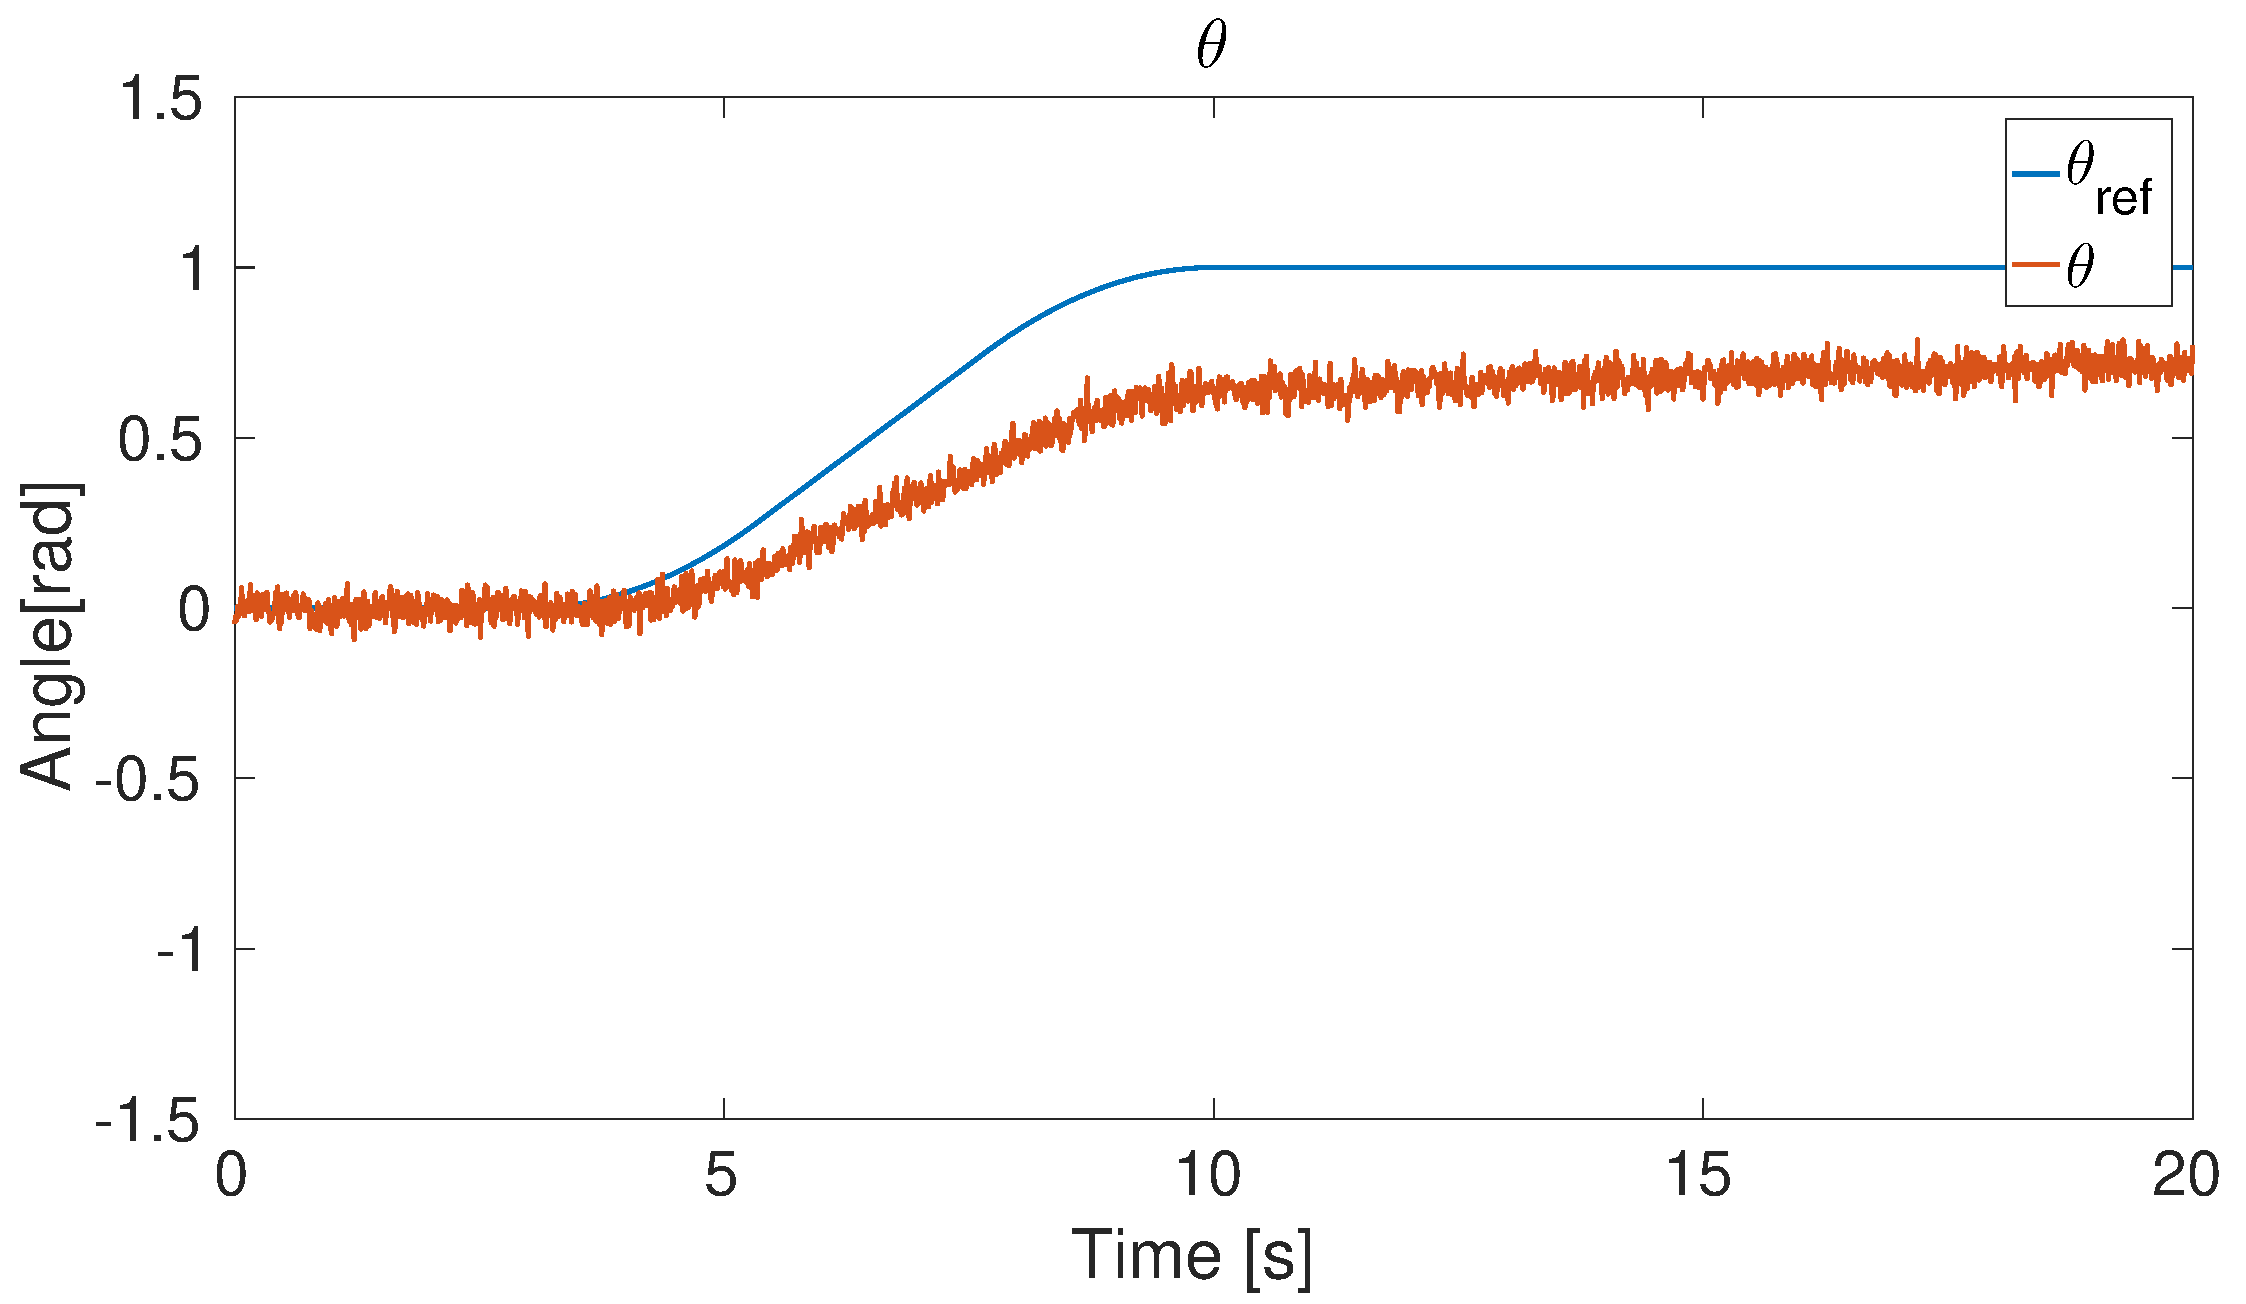
\includegraphics[width=0.4\textwidth]{simStepAllThetas3e10a1}}
  \qquad
  \subfloat[][\label{fig:TestStepAllYawAttitude} A smooth step applied in $\yawAngle$.]{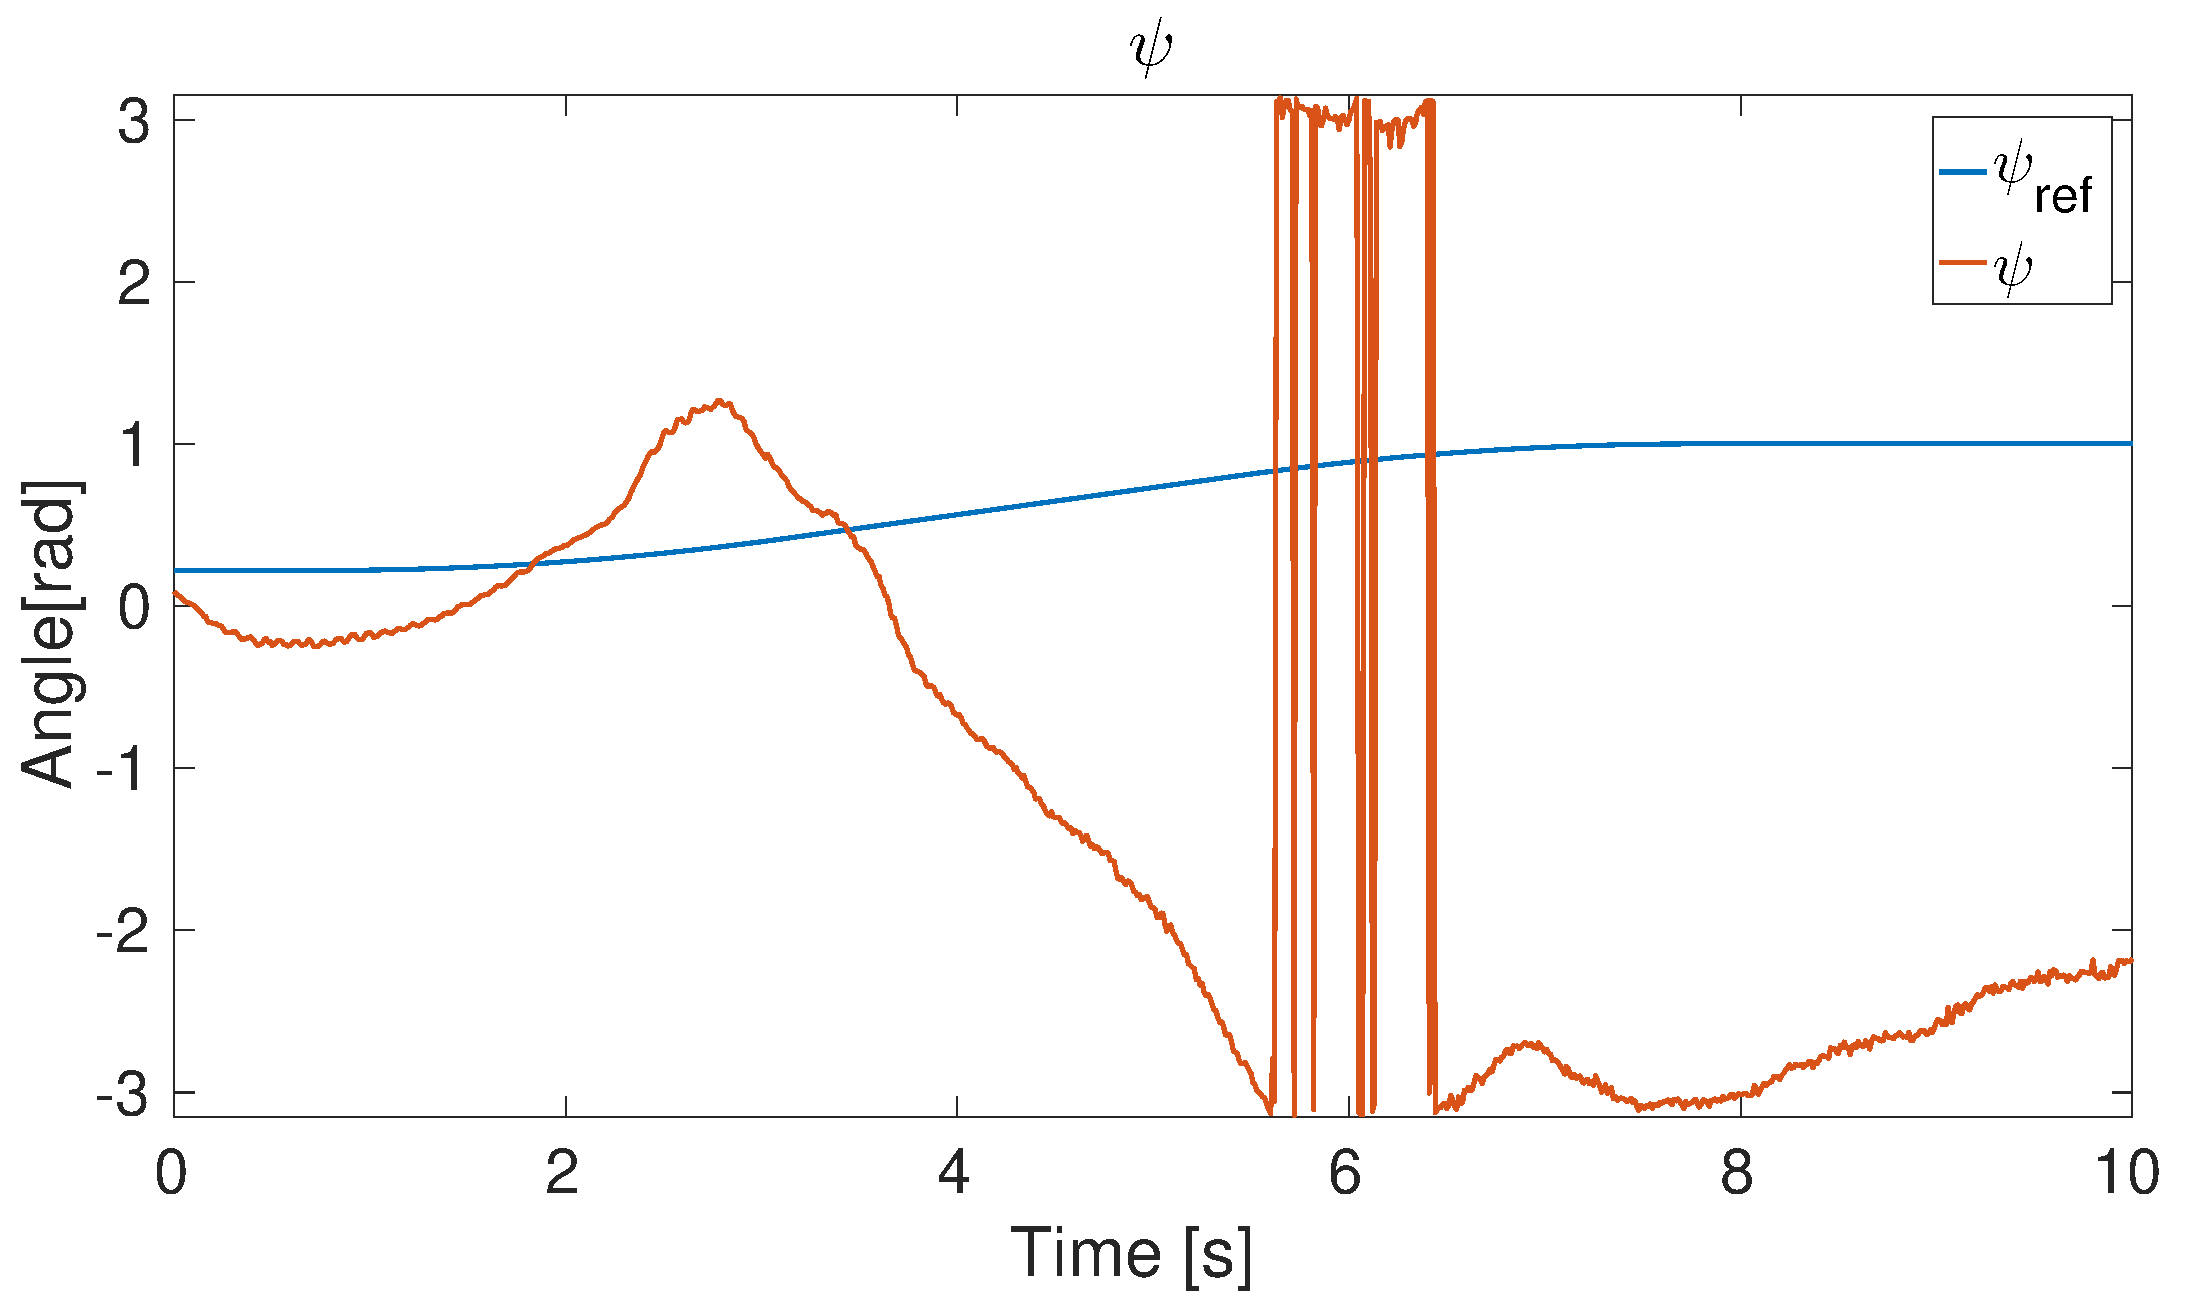
\includegraphics[width=0.4\textwidth]{testStepAllPsis3e10a1}}
  \qquad
  \subfloat[][\label{fig:simStepAllYawAttitude} A smooth step applied to the simulated \abbrROV in $\yawAngle$.]{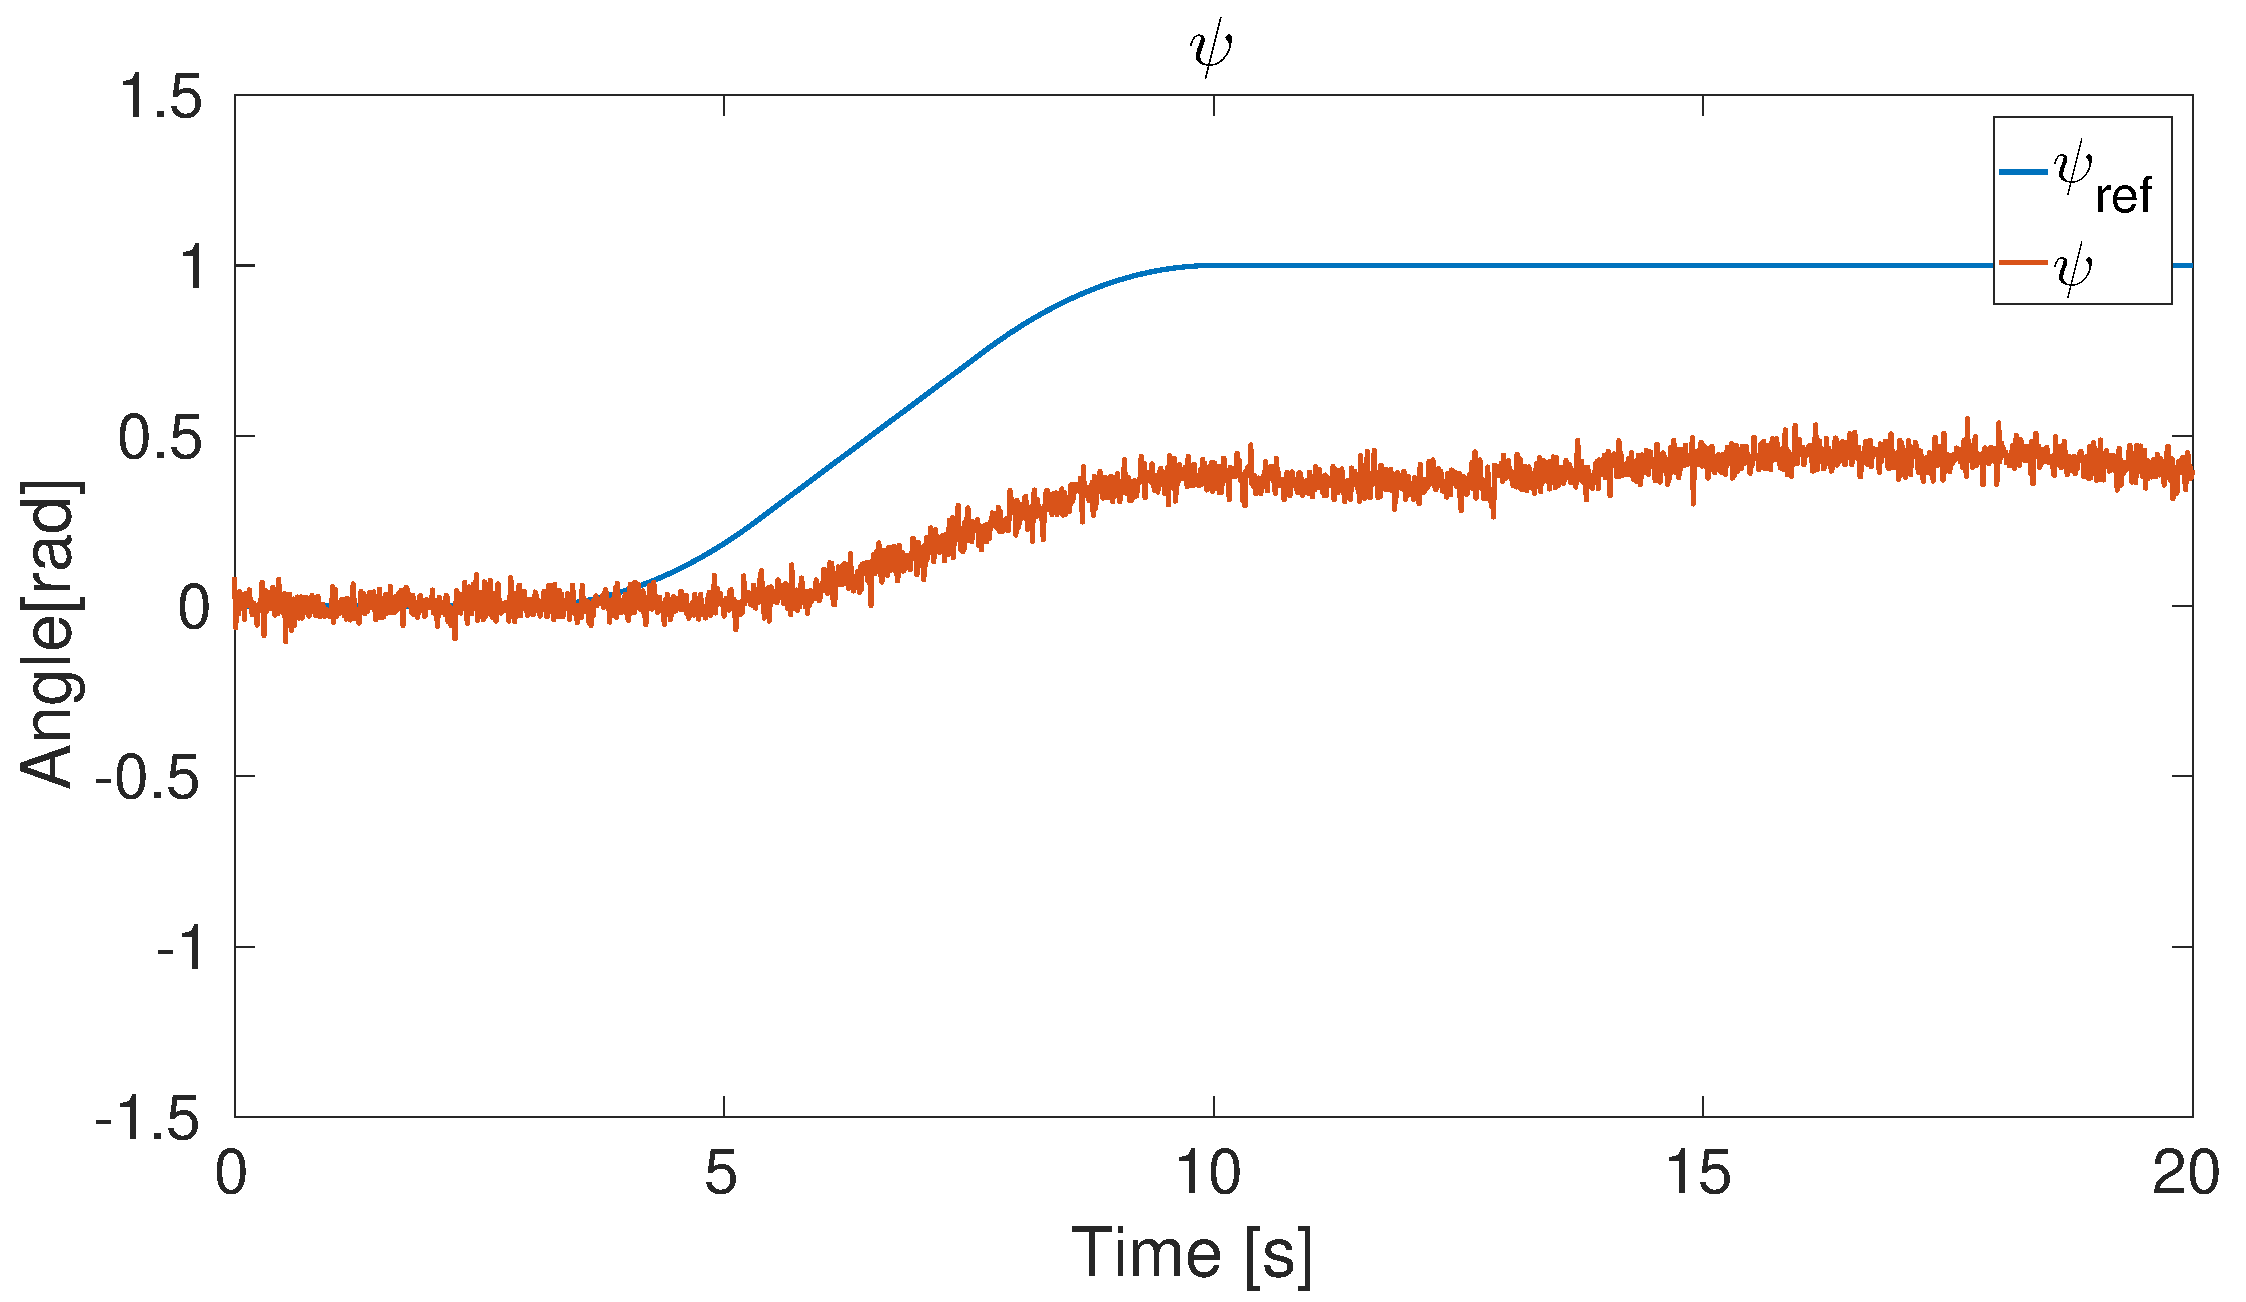
\includegraphics[width=0.4\textwidth]{simStepAllPsis3e10a1}}
  \caption{\label{fig:StepAllAttitude}% 
  Smooth steps were applied in all attitude angles at the same time while using the attitude controller.}
\end{figure}

\Figureref{fig:StepAllAttitude} shows smooth step reference signals applied in all attitude angles while using the attitude controller. Initially did $\rollAngle$ and $\pitchAngle$ follow the reference signals well in the real test. The $\rollAngle$ oscillated with a steady state error of 0.9 in the real test. However, $\pitchAngle$ was kept closer to the reference signal with a steady state error of 0.4. The attitude angle $\yawAngle$ could not be stabilised during the real test and drifted throughout the test. In the simulated test case did not the attitude angles reach the reference signal. The attitude angle $\pitchAngle$ had a steady state error of 0.3 and the other angles had a steady state error of 0.5.

\begin{figure}
\centering
  \subfloat[][\label{fig:testSinAllRollAttitude} A sine signal with amplitude $1$ and frequency $0.5\hertz$ applied in $\rollAngle$.]{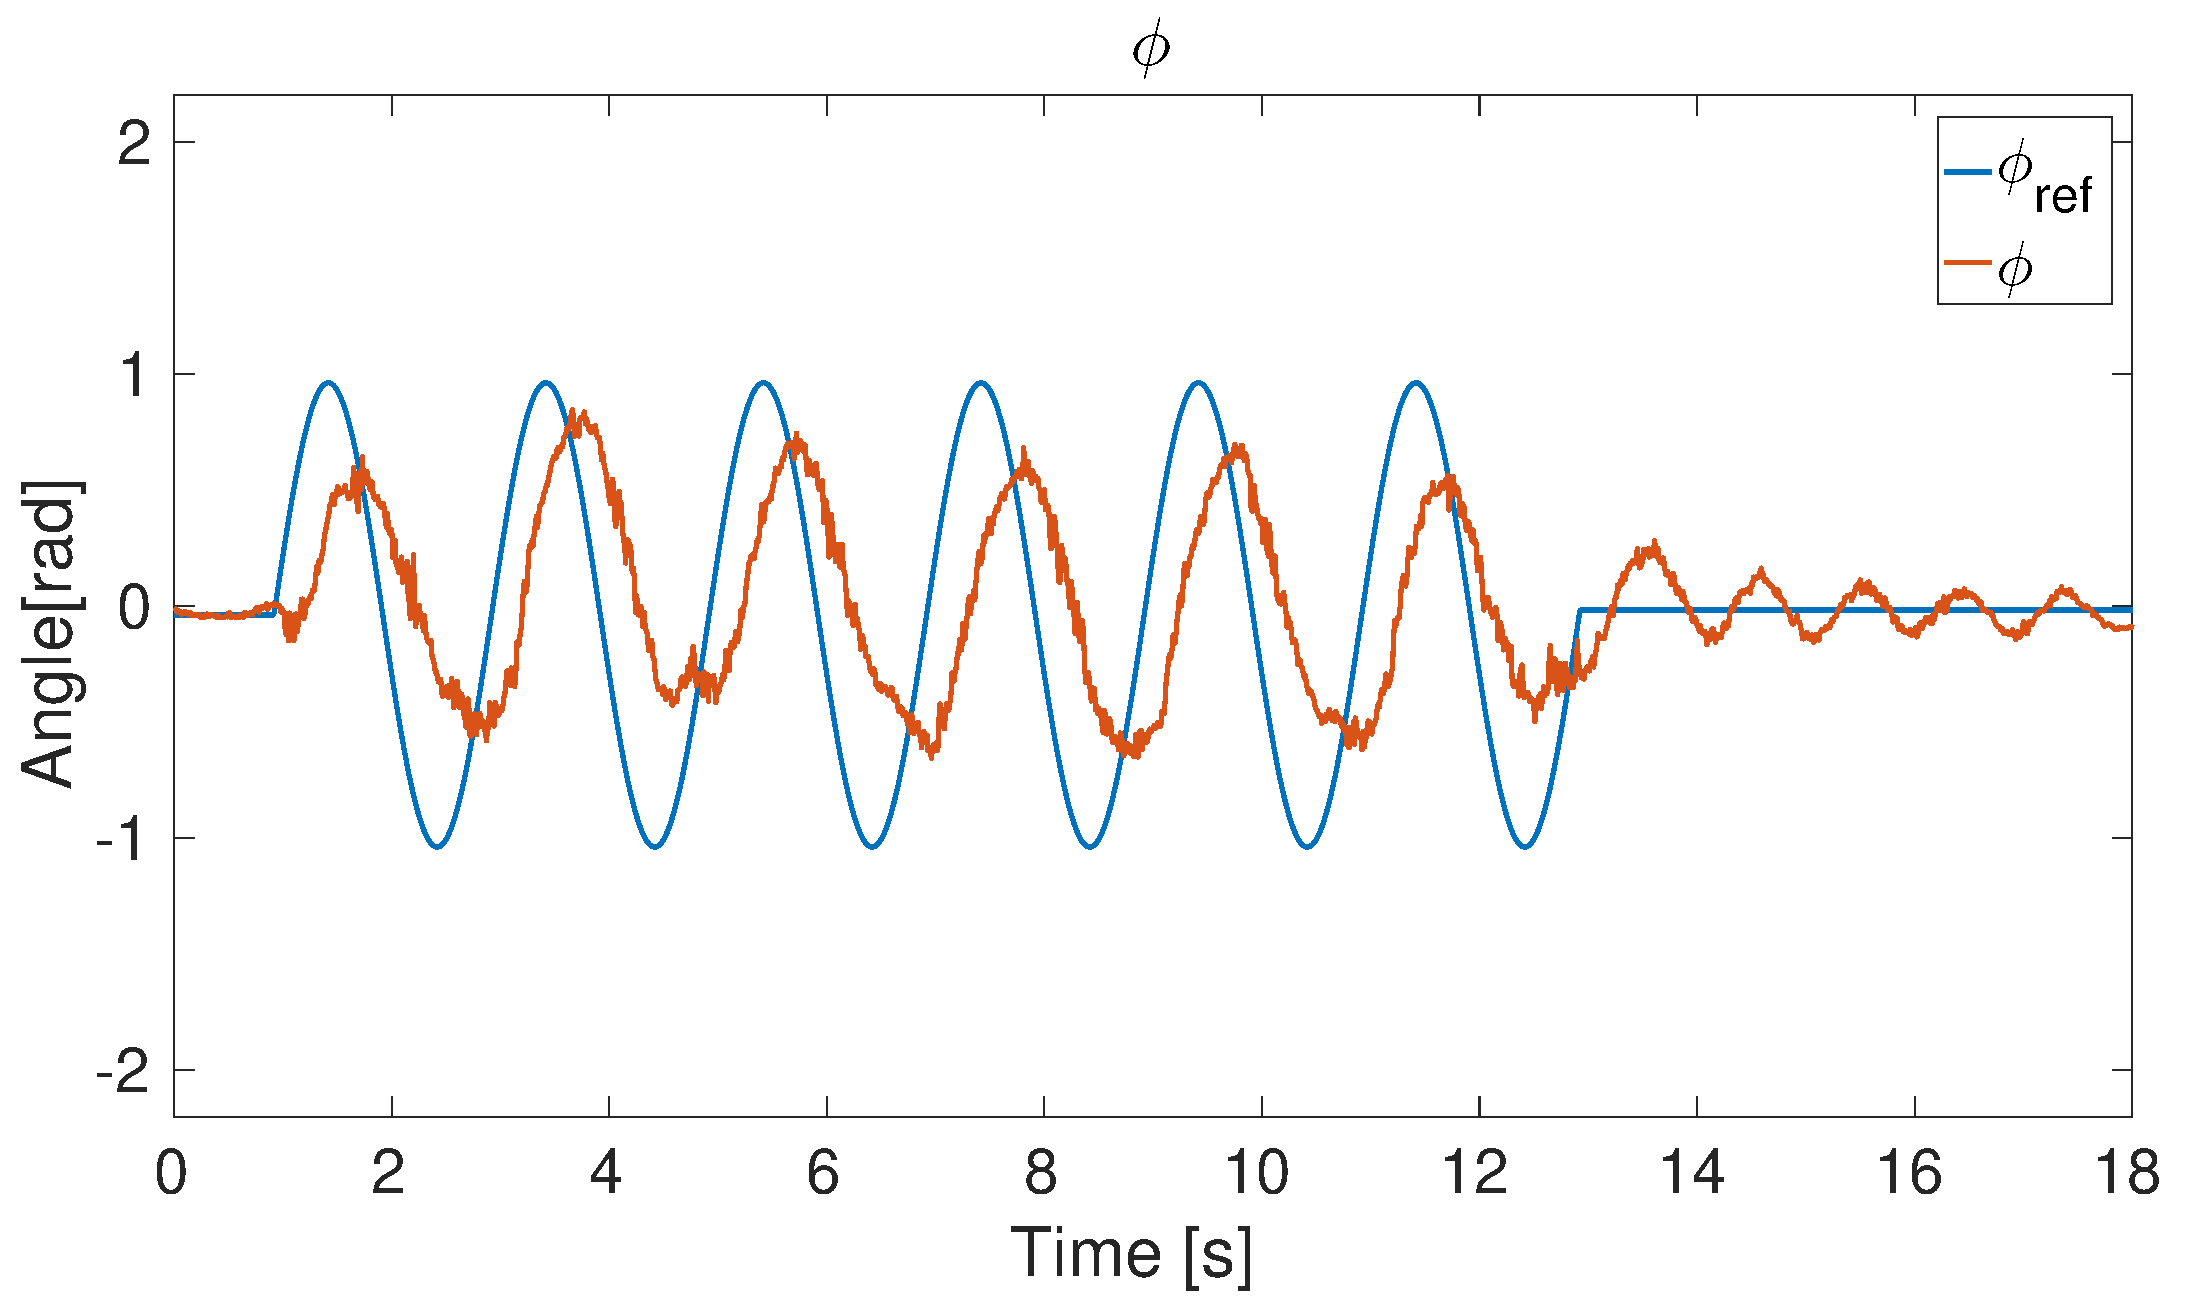
\includegraphics[width=0.4\textwidth]{testSinAllPhiA1}}
  \qquad
  \subfloat[][\label{fig:simSinAllRollAttitude} A sine signal with amplitude $1$ and frequency $0.5\hertz$ applied to the simulated \abbrROV in $\rollAngle$.]{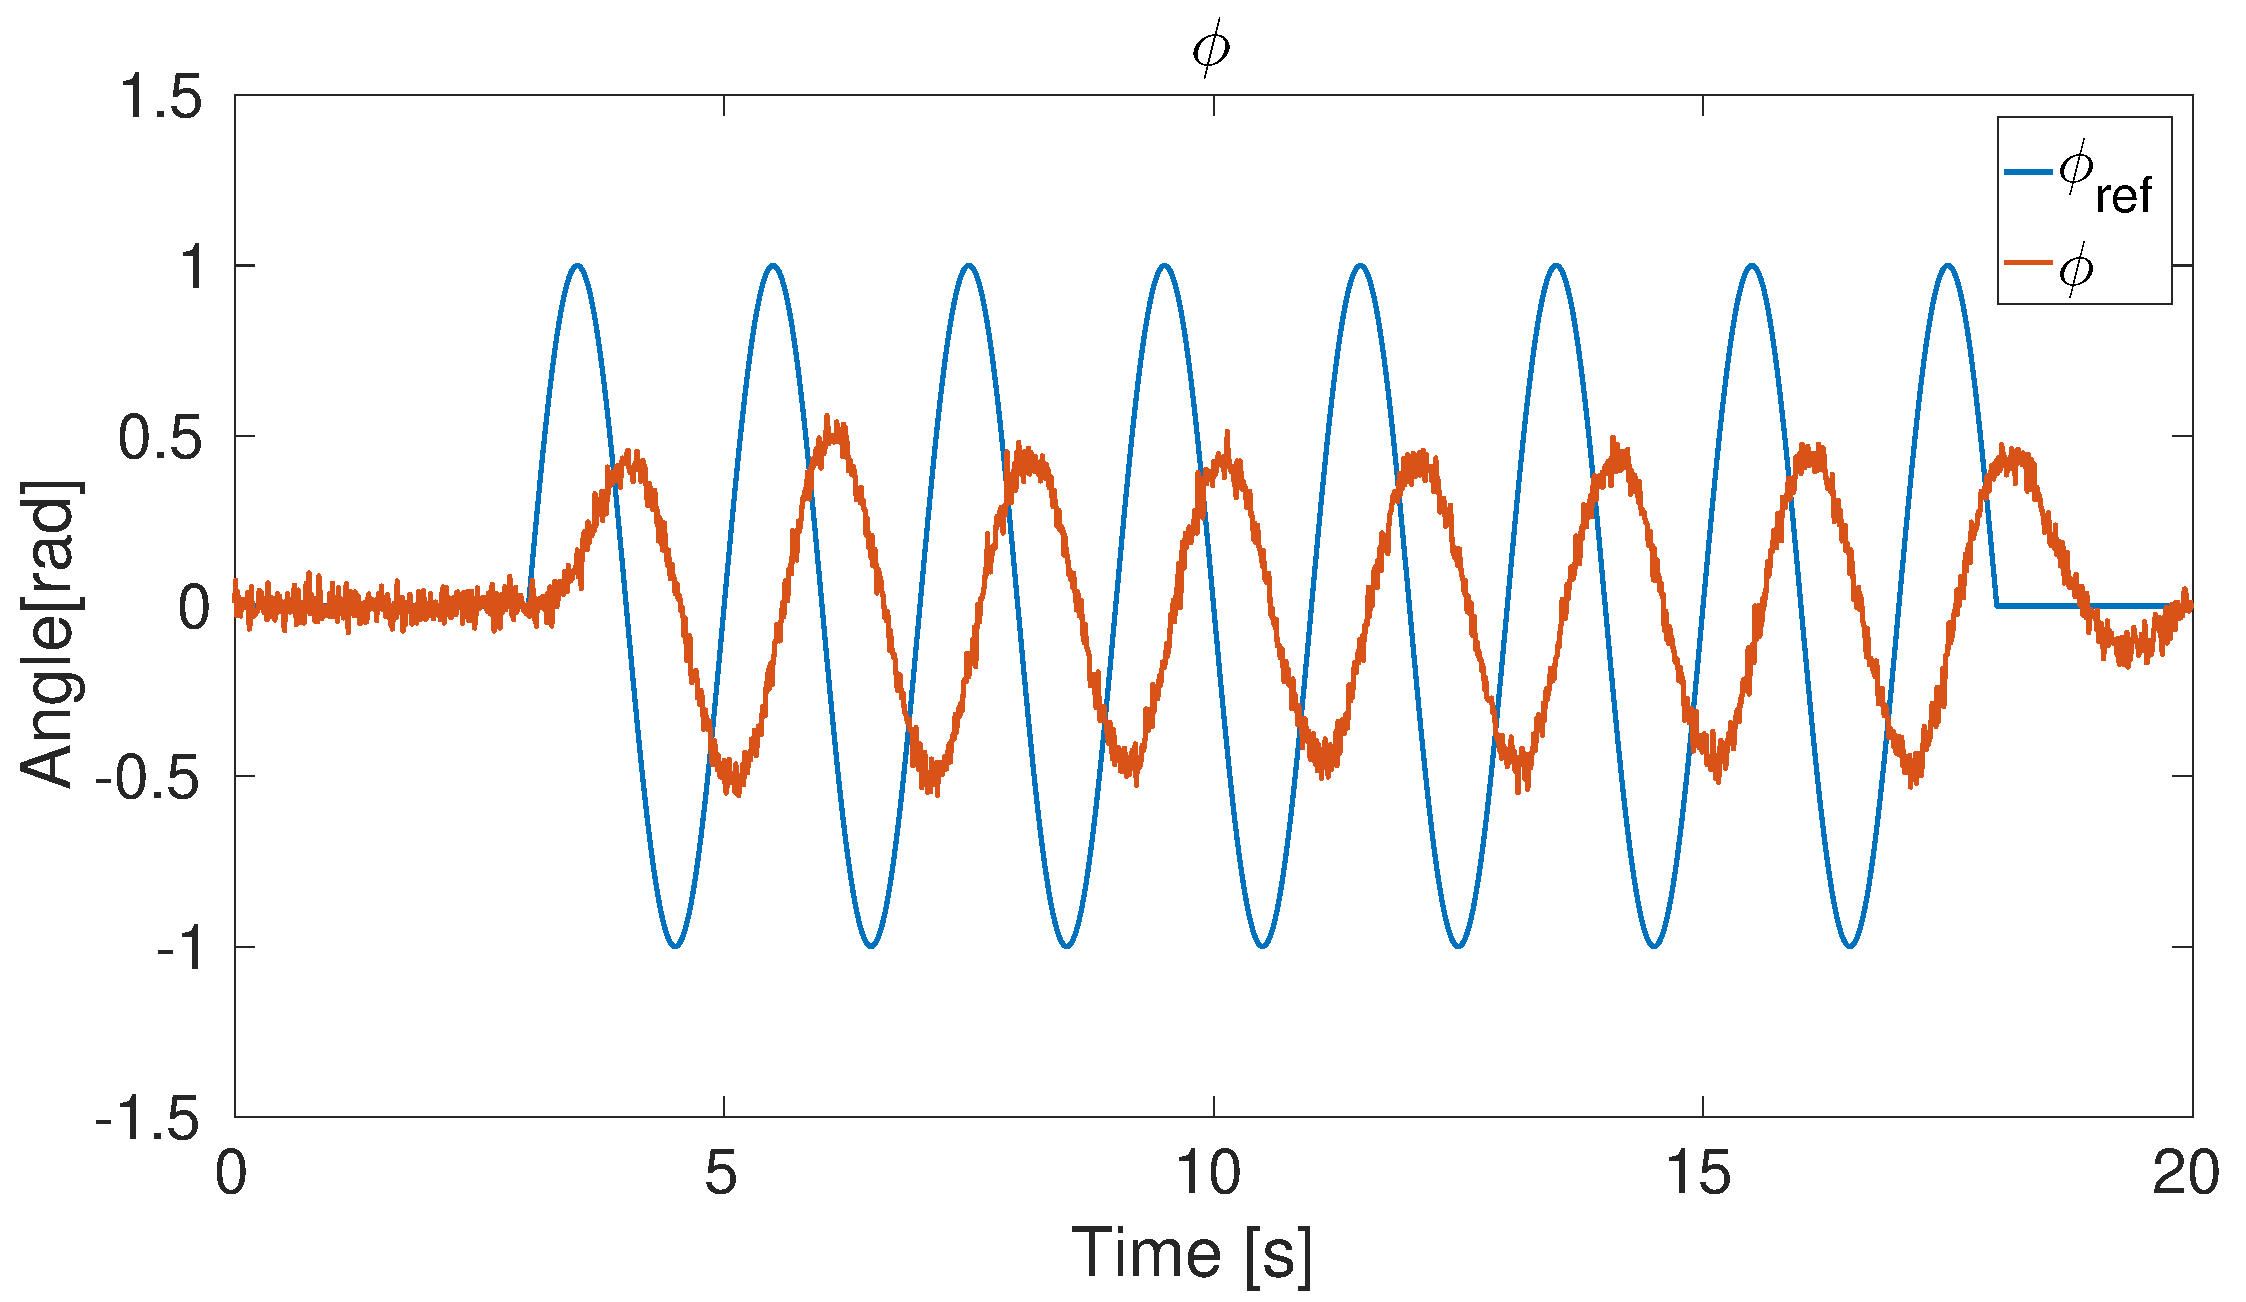
\includegraphics[width=0.4\textwidth]{simSinAllPhiA1}}
  \qquad
  \subfloat[][\label{fig:testSinAllPitchAttitude} A sine signal with amplitude $1$ and frequency $0.5\hertz$ applied in $\pitchAngle$.]{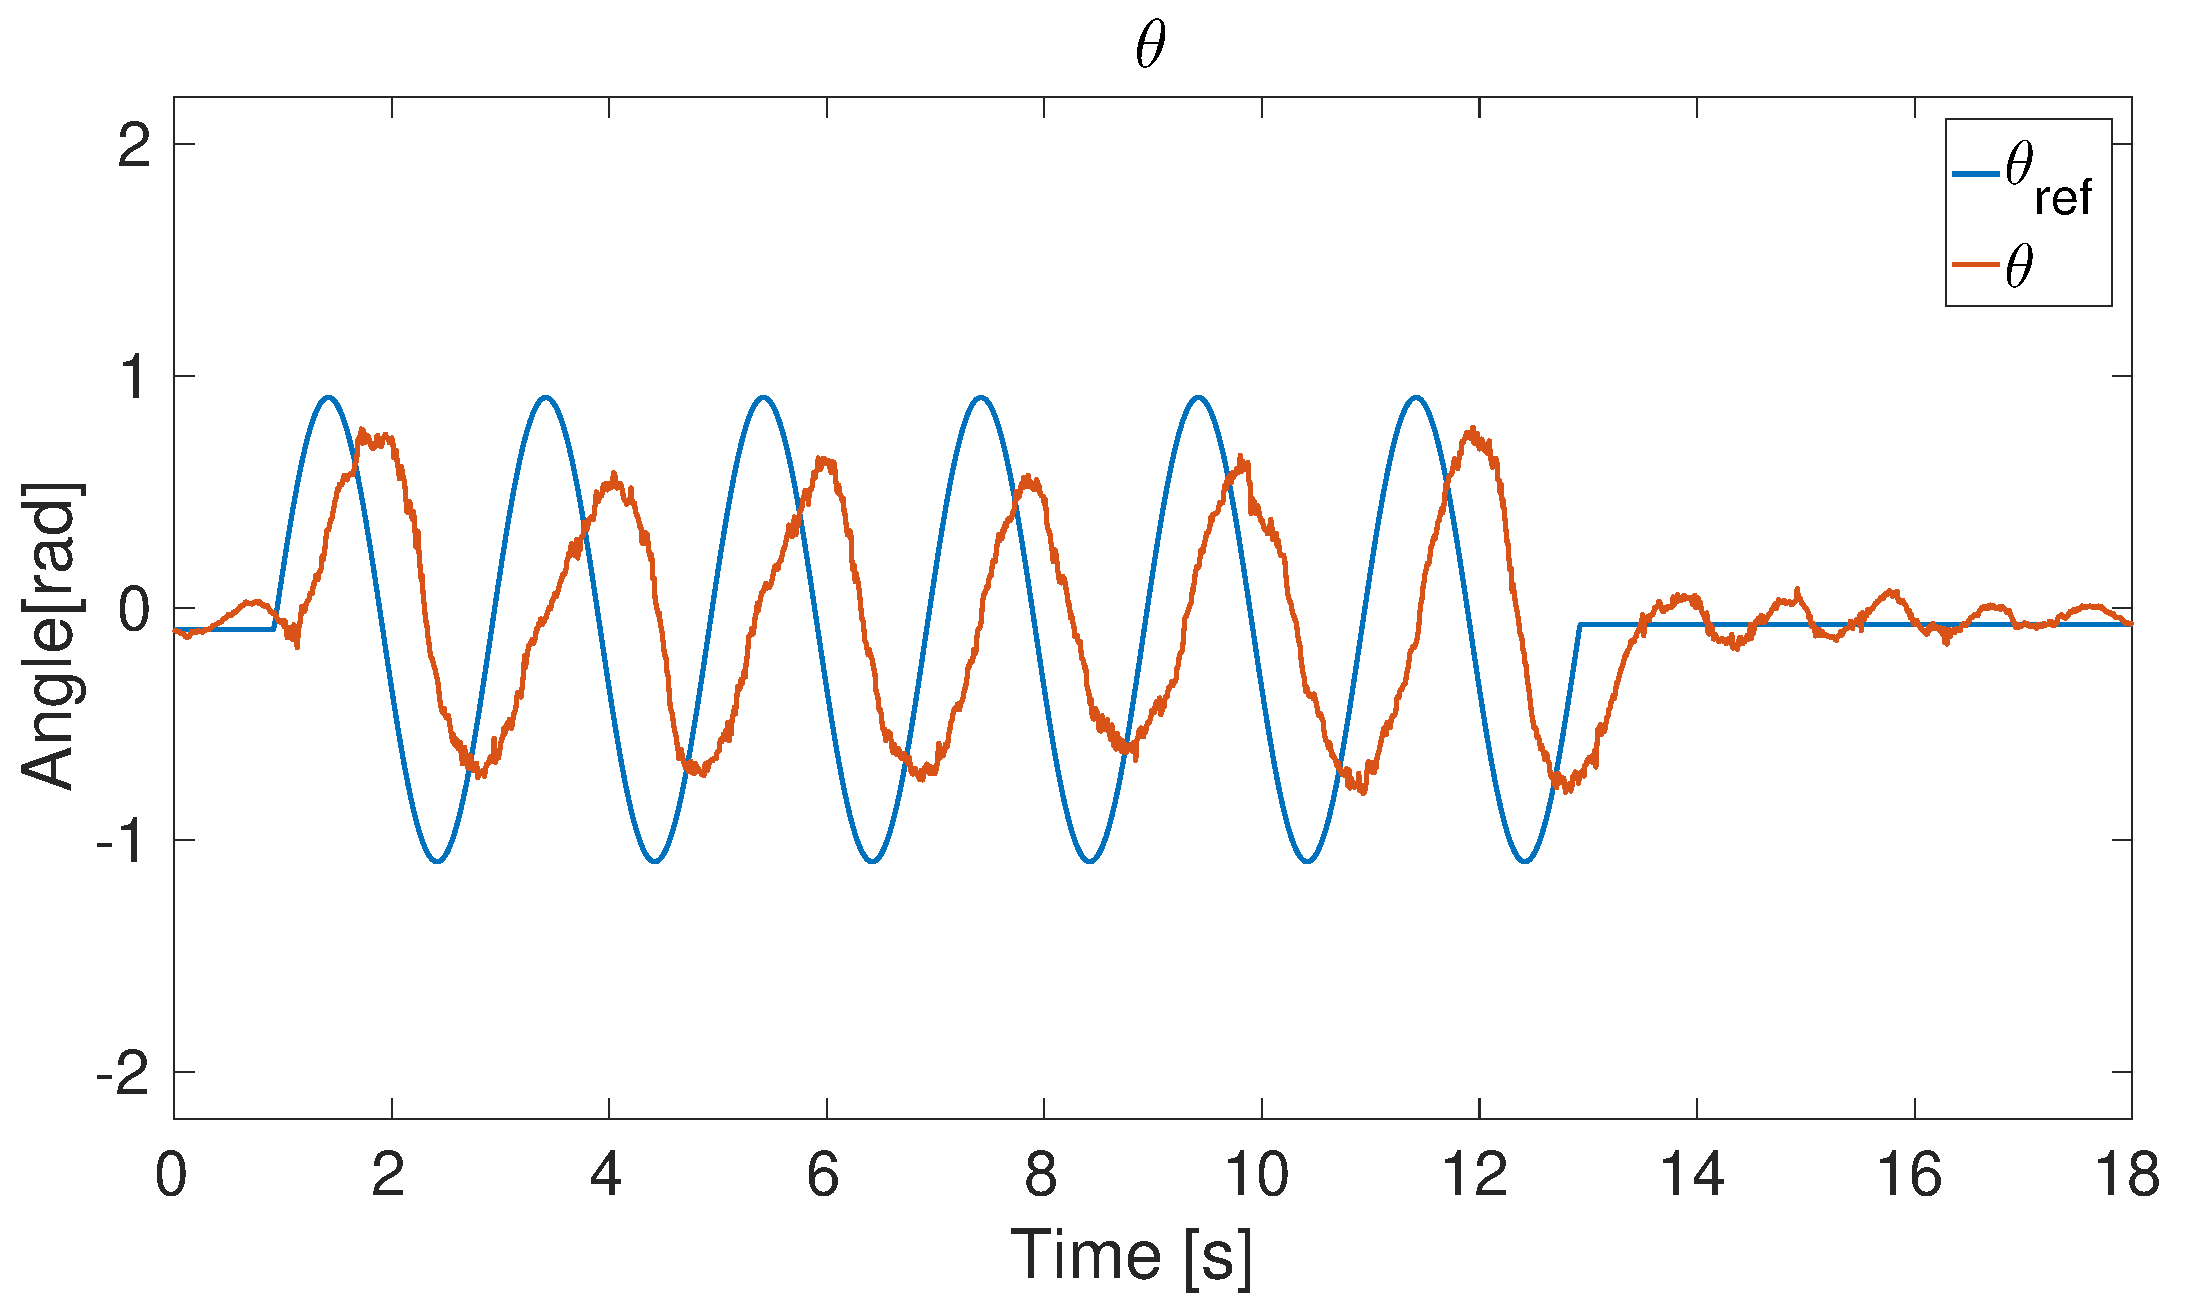
\includegraphics[width=0.4\textwidth]{testSinAllThetaA1}}
  \qquad
  \subfloat[][\label{fig:simSinAllPitchAttitude} A sine signal with amplitude $1$ and frequency $0.5\hertz$ applied to the simulated \abbrROV in $\pitchAngle$.]{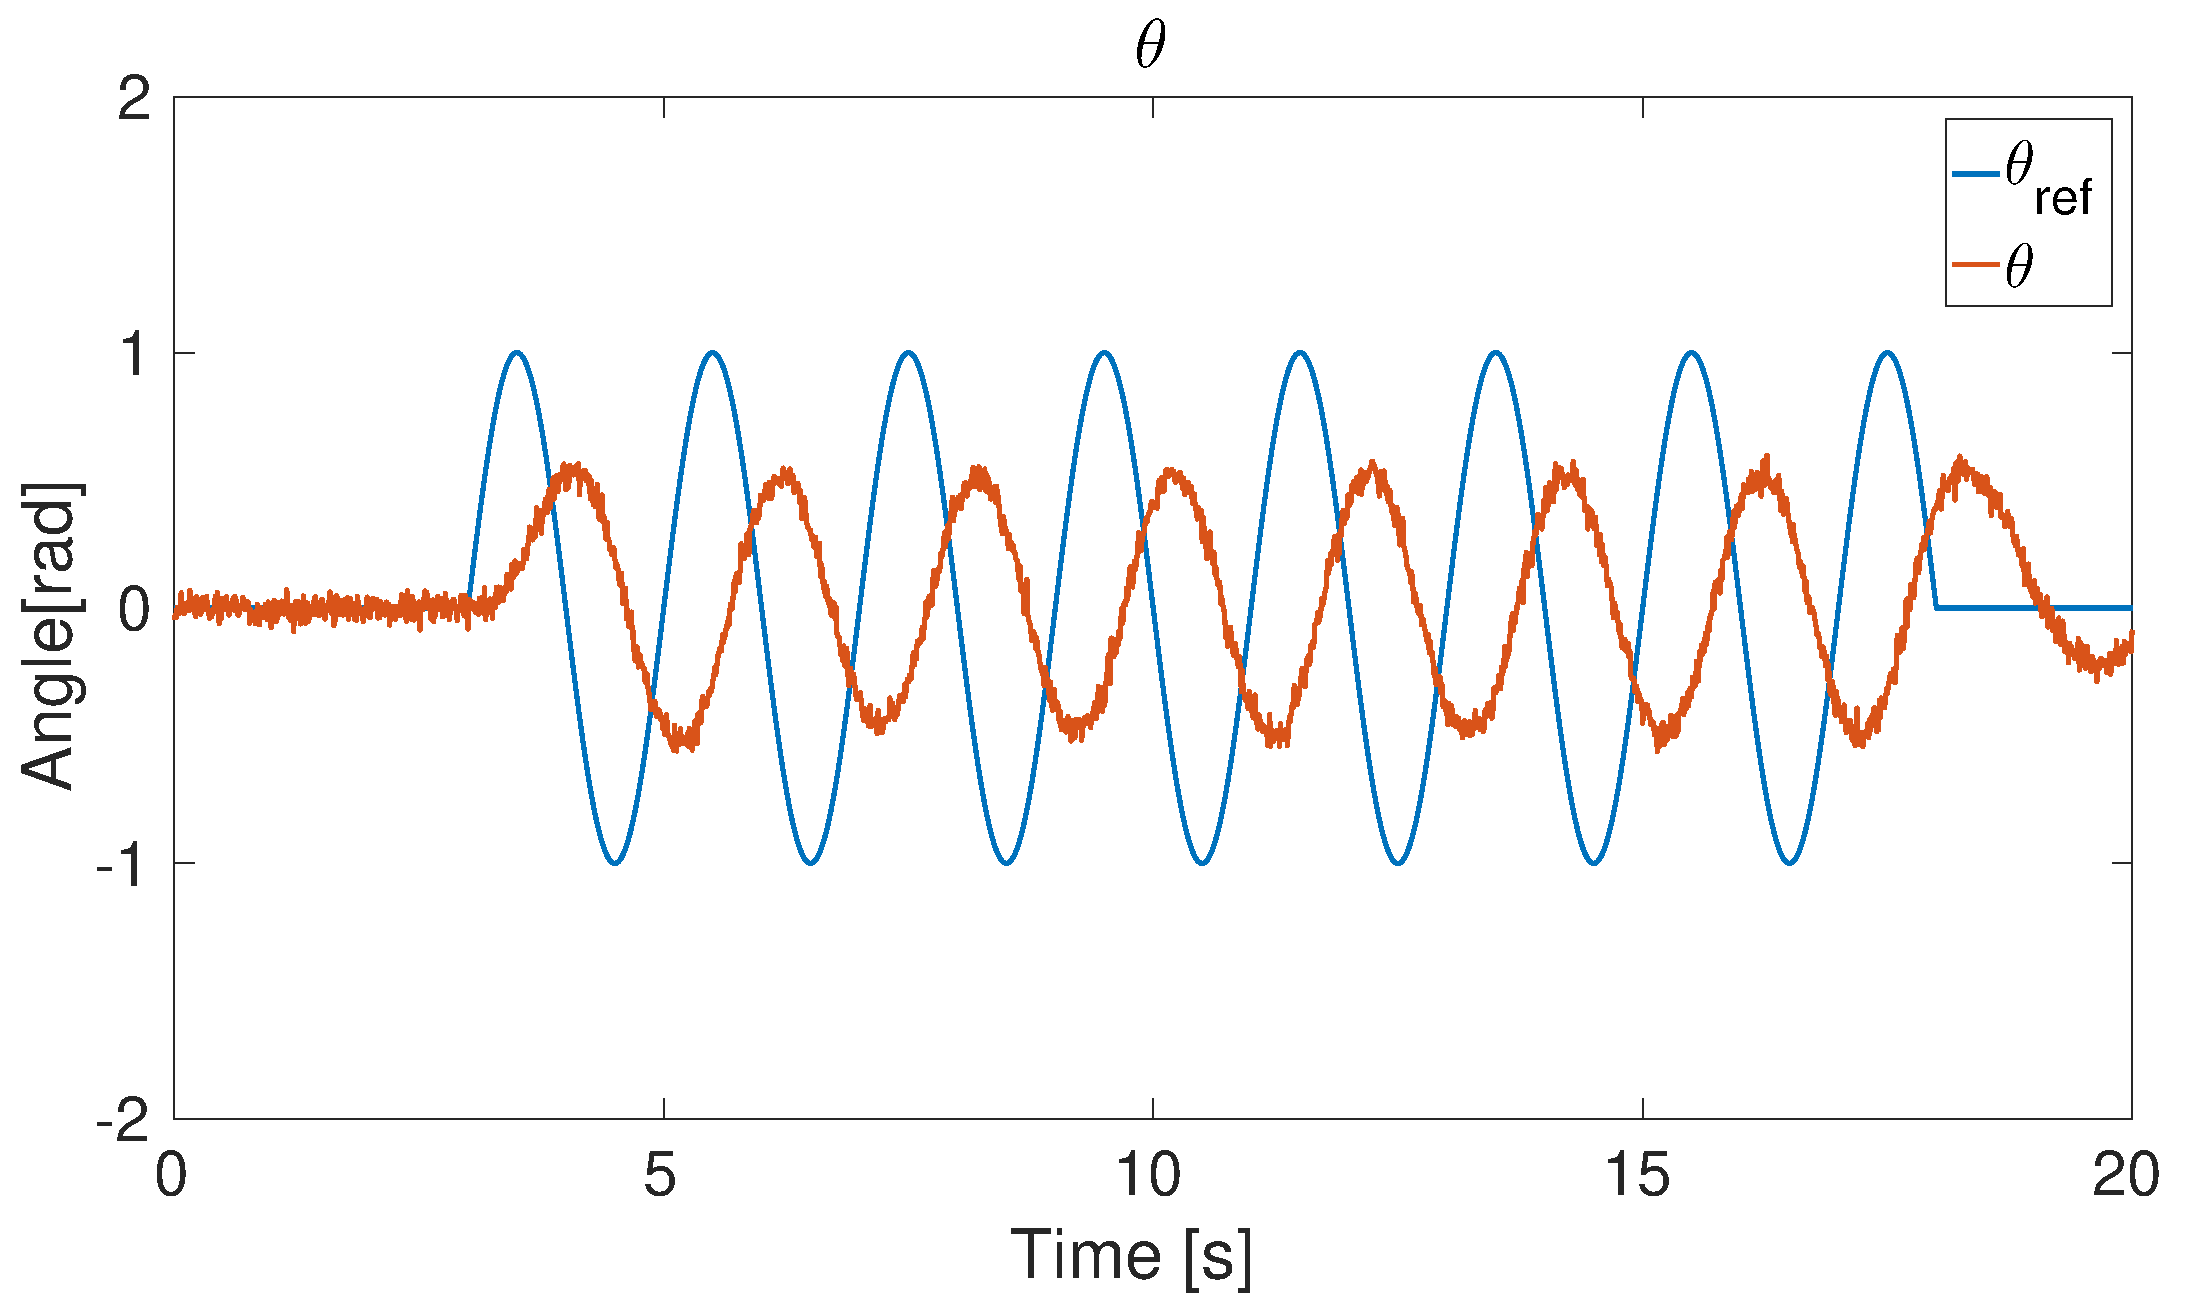
\includegraphics[width=0.4\textwidth]{simSinAllThetaA1}}
  \qquad
  \subfloat[][\label{fig:testSinAllYawAttitude} A sine signal with amplitude $1$ and frequency $0.5\hertz$ applied in $\yawAngle$.]{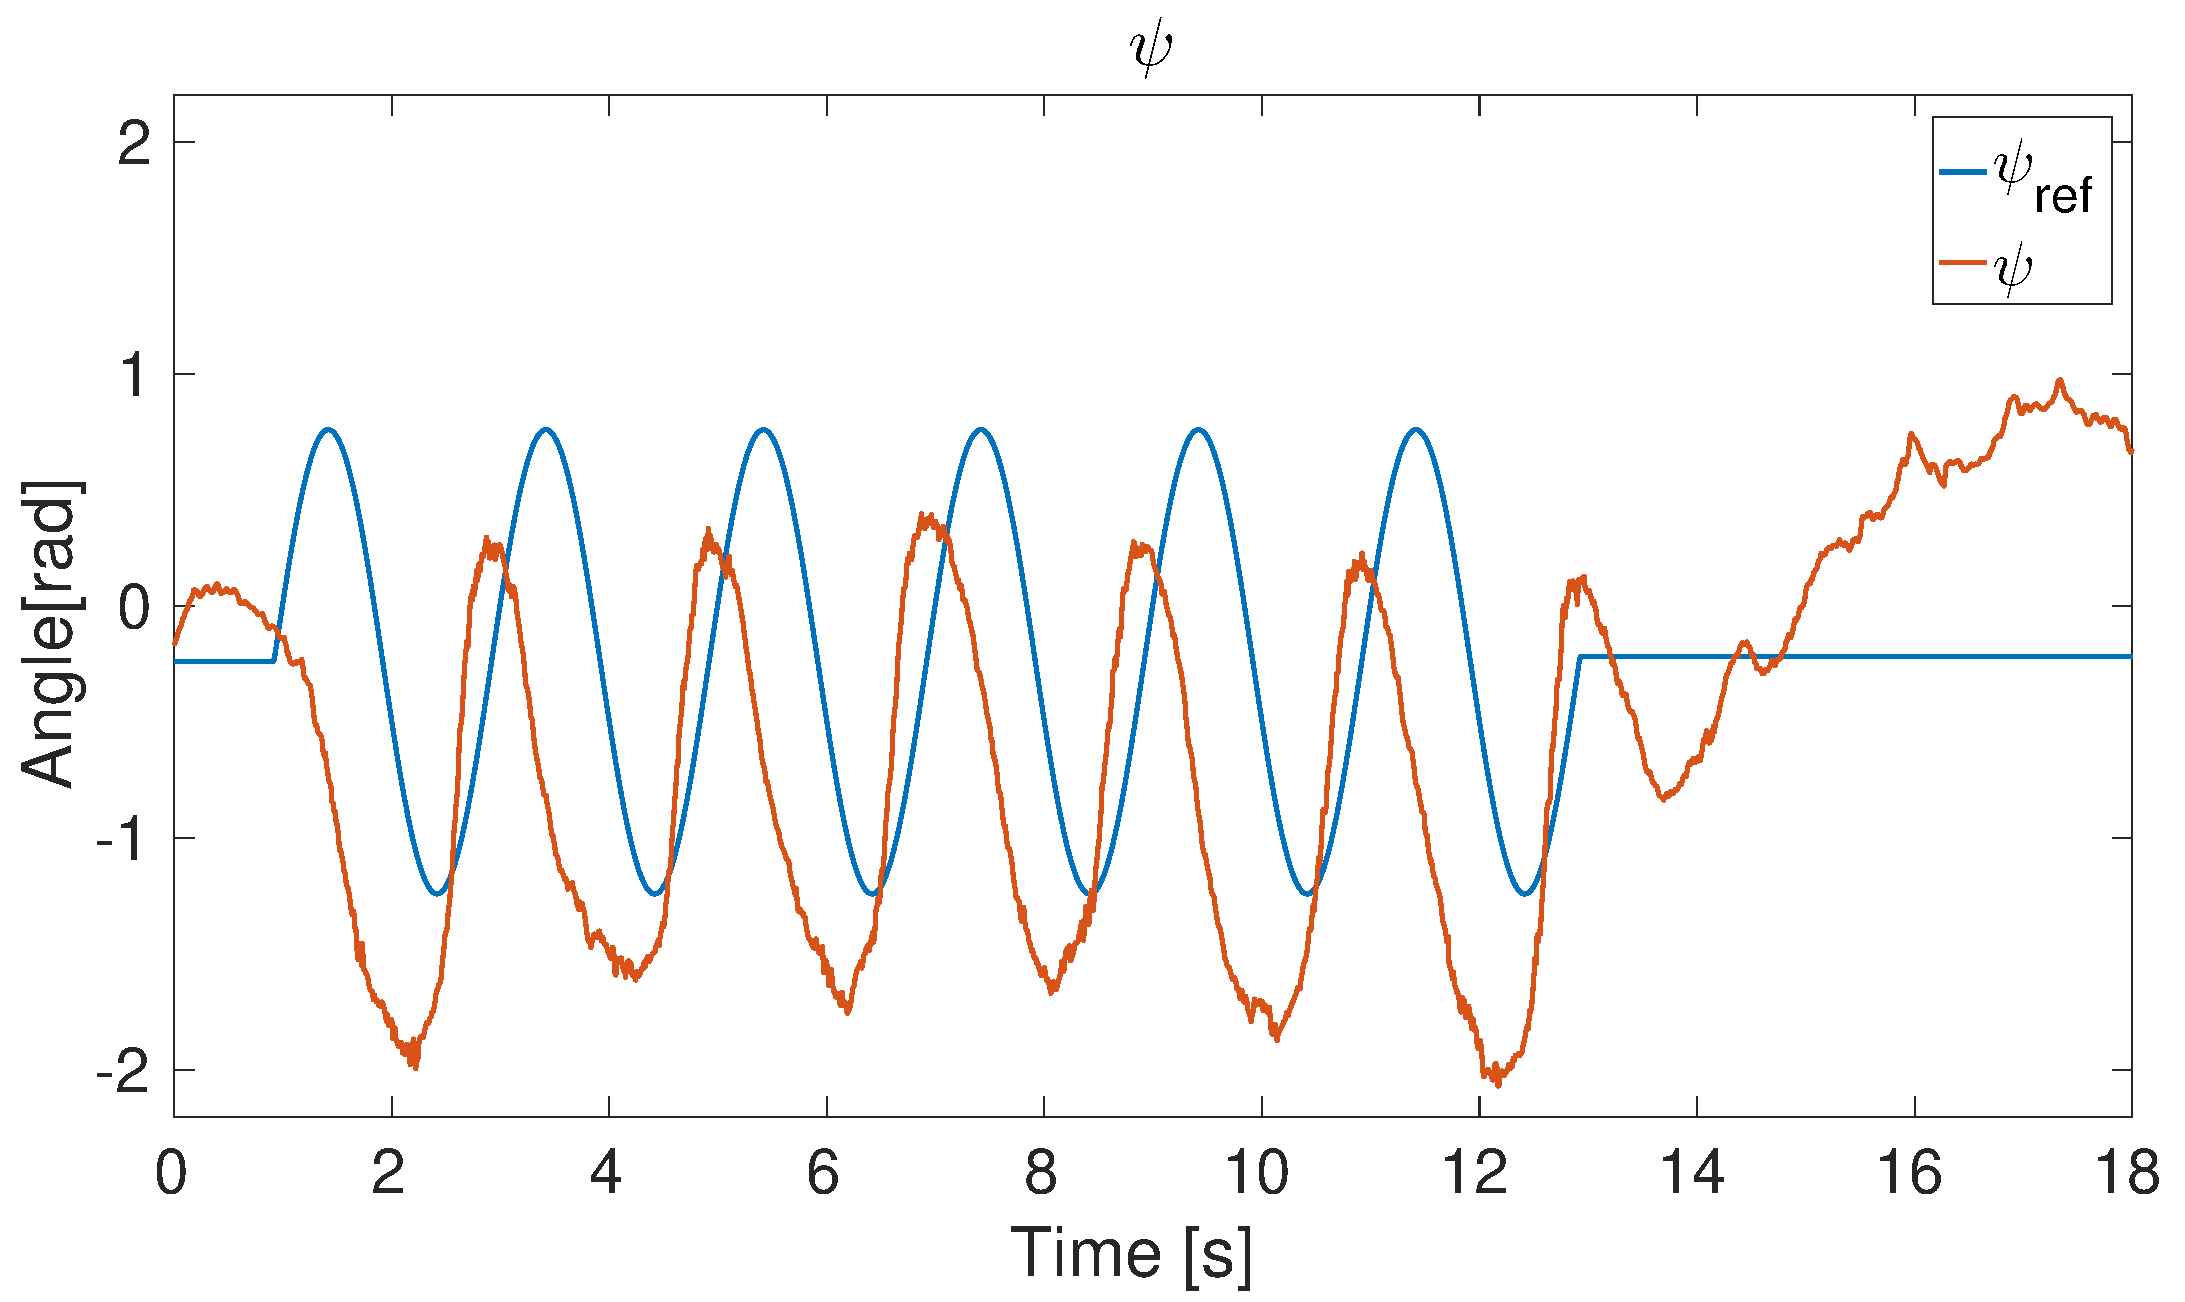
\includegraphics[width=0.4\textwidth]{testSinAllPsiA1}}
  \qquad
  \subfloat[][\label{fig:simSinAllYawAttitude} A sine signal with amplitude $1$ and frequency $0.5\hertz$ applied to the simulated \abbrROV in $\yawAngle$.]{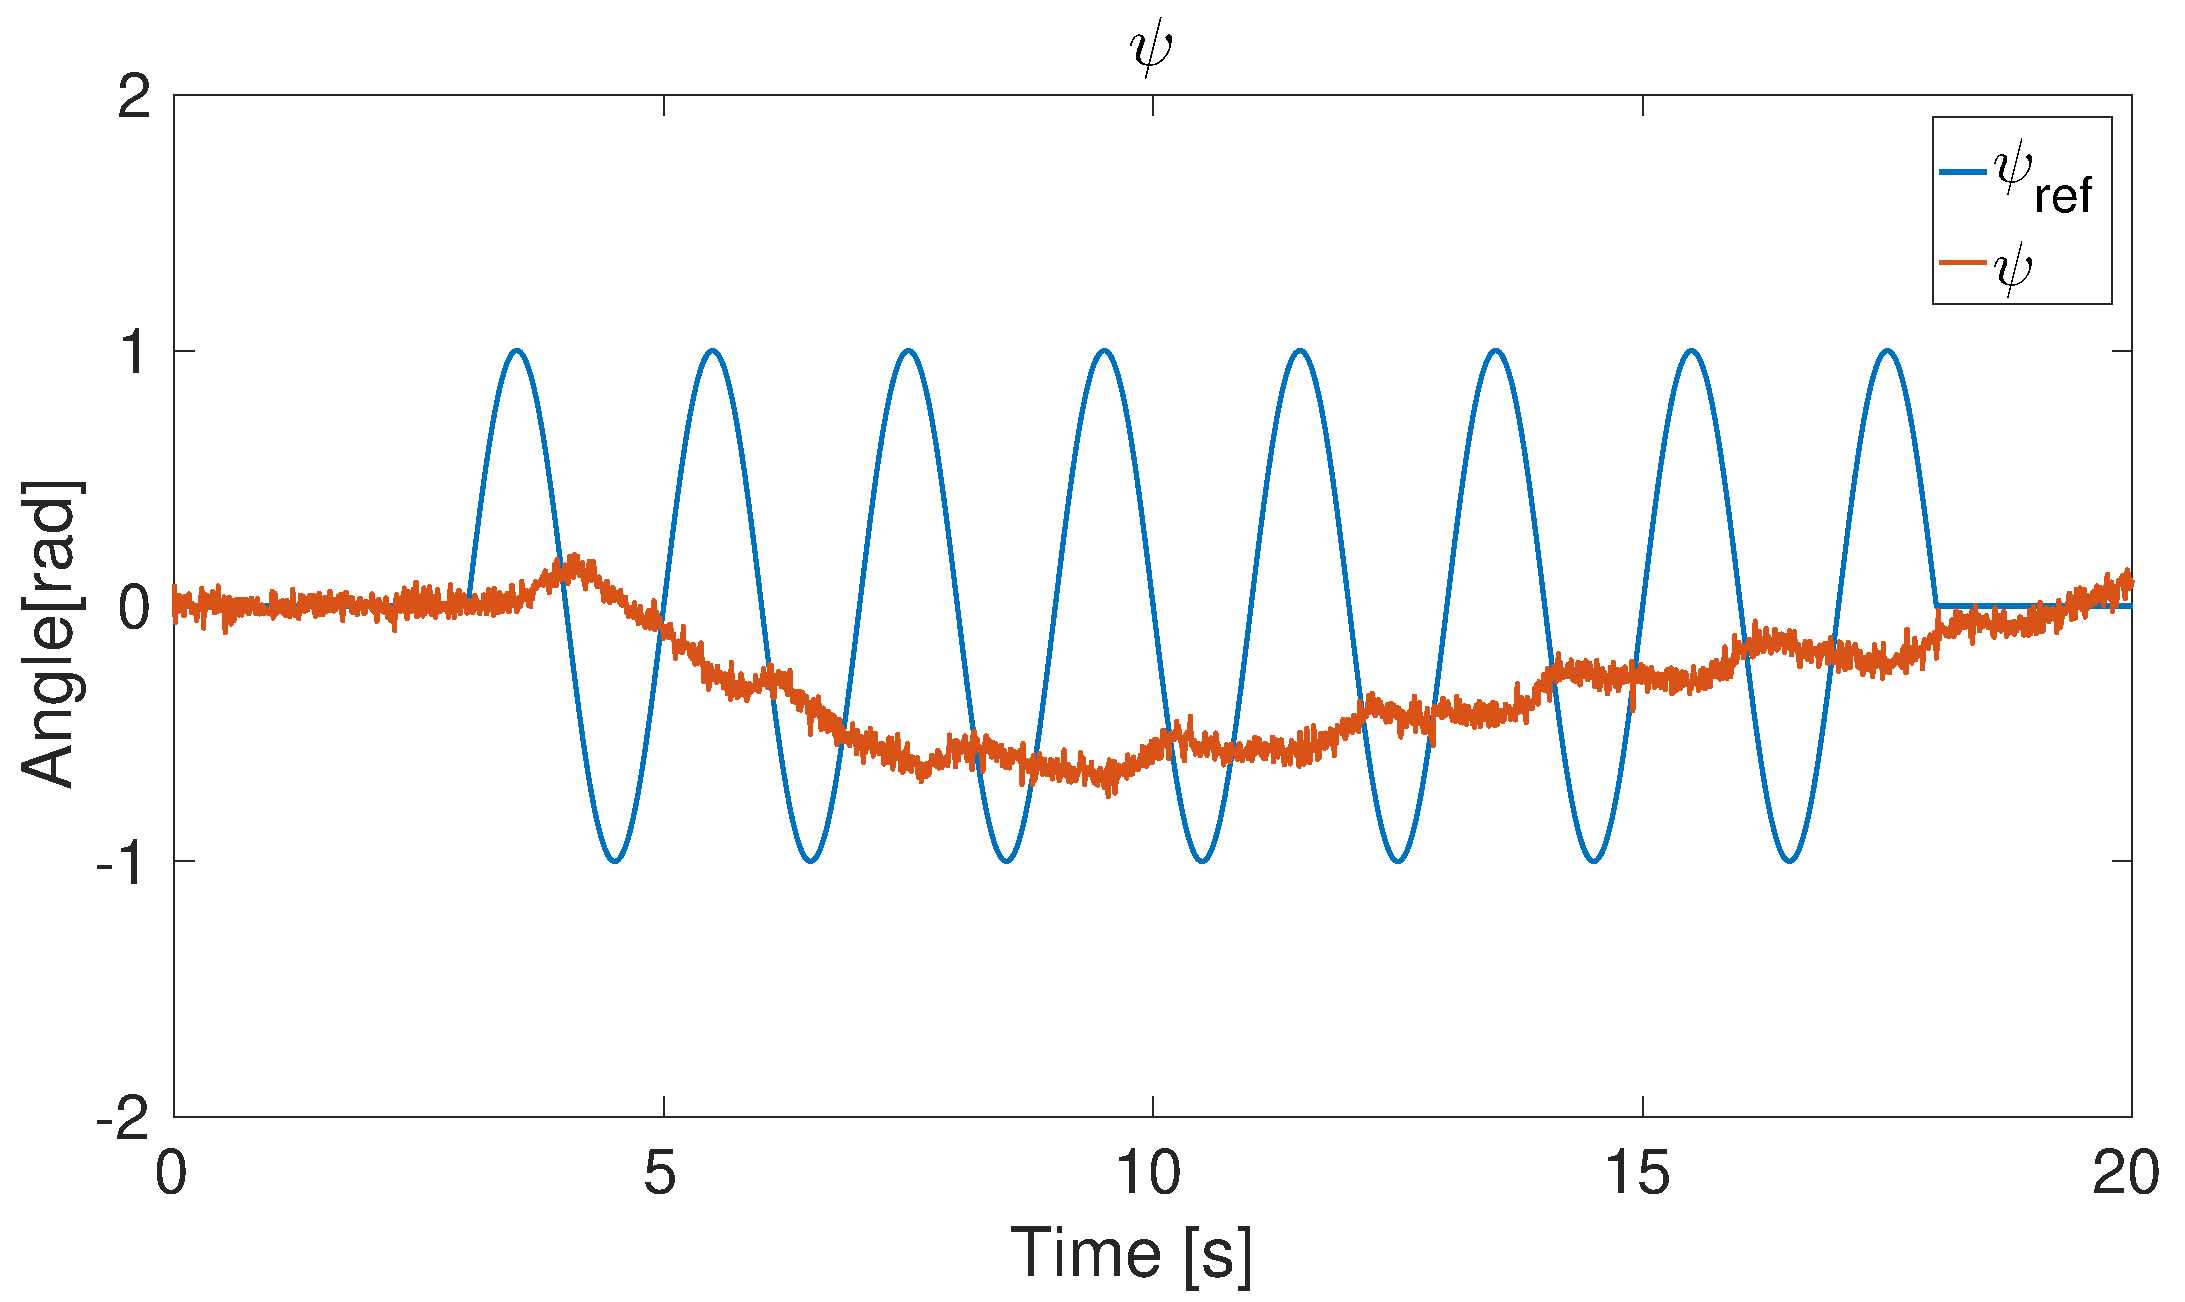
\includegraphics[width=0.4\textwidth]{simSinAllPsiA1}}
  \caption{\label{fig:SinAllAttitude}%
  Sine signals were applied in all attitude angles at the same time while using the attitude controller.}
\end{figure}

Sine reference signals with amplitude 1 and frequency $0.5 \hertz$ can be seen in \Figureref{fig:SinAllAttitude}. The angles $\rollAngle$ and $\pitchAngle$ did not reached the assigned amplitude in the real test. However, did they have the general form of a sine but phase shifted relative to the reference signals. The $\yawAngle$ follows the reference signal well but with a phase shift and a bias. In simulation tests the same phase shift and lack of amplitude happened in $\rollAngle$ and $\pitchAngle$. The simulated result in $\yawAngle$ did not follow the reference signal at all. 

\begin{figure}
\centering
  \subfloat[][\label{fig:testStepPhiTheta05RollAttitude} A smooth step applied in $\rollAngle$.]{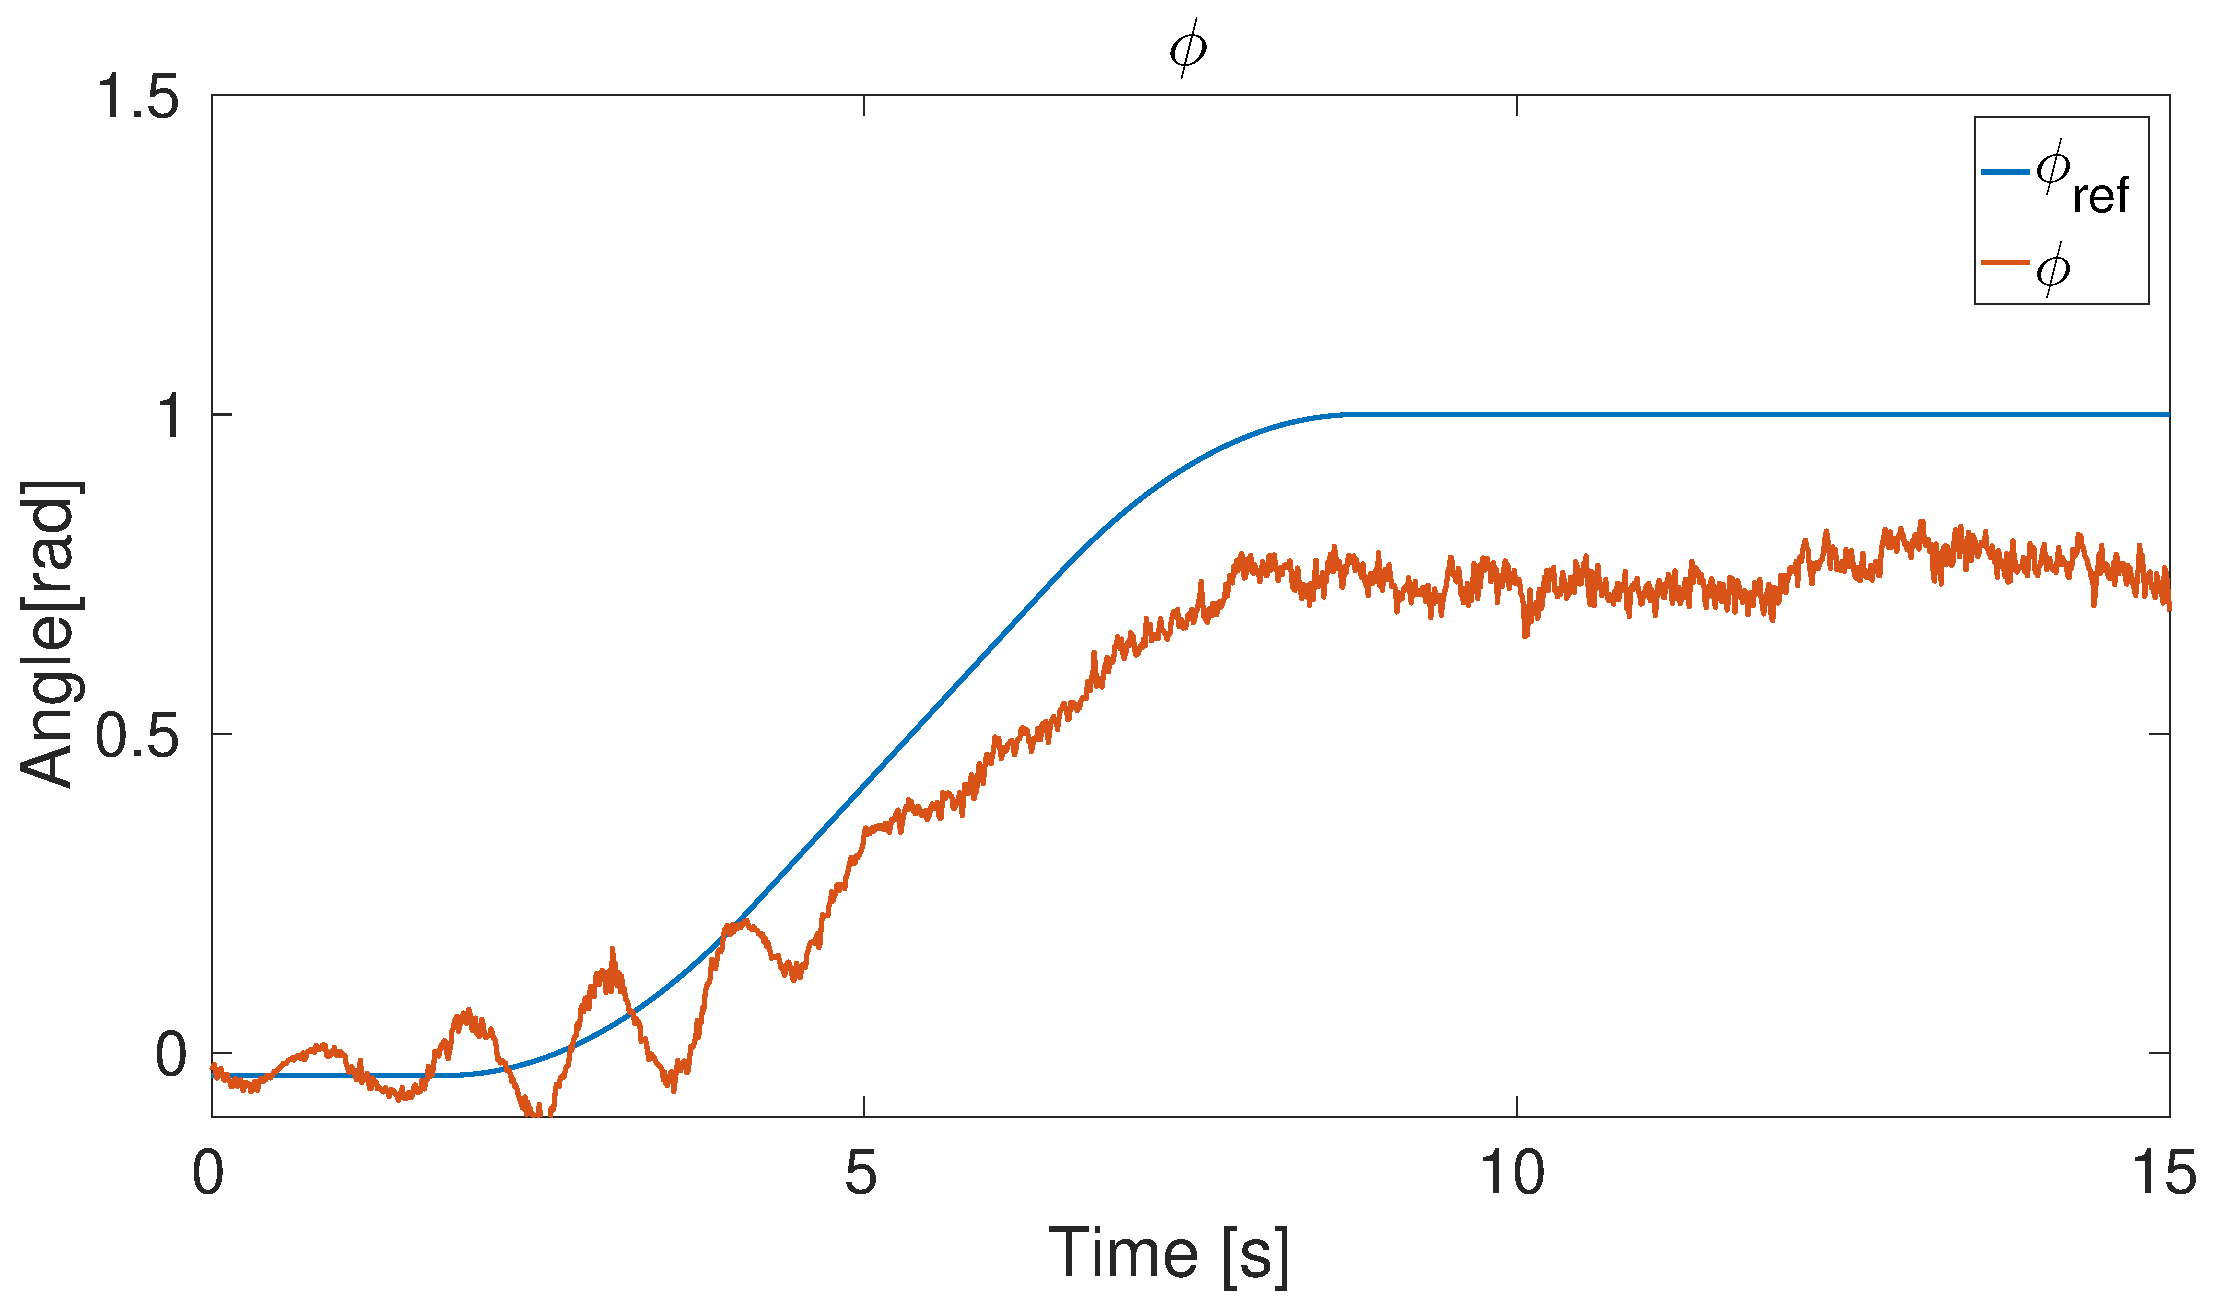
\includegraphics[width=0.4\textwidth]{testStepThetaPhiPhis3e10a1}}
  \qquad
  \subfloat[][\label{fig:simStepPhiTheta05RollAttitude} A smooth step applied to the simulated \abbrROV in $\rollAngle$.]{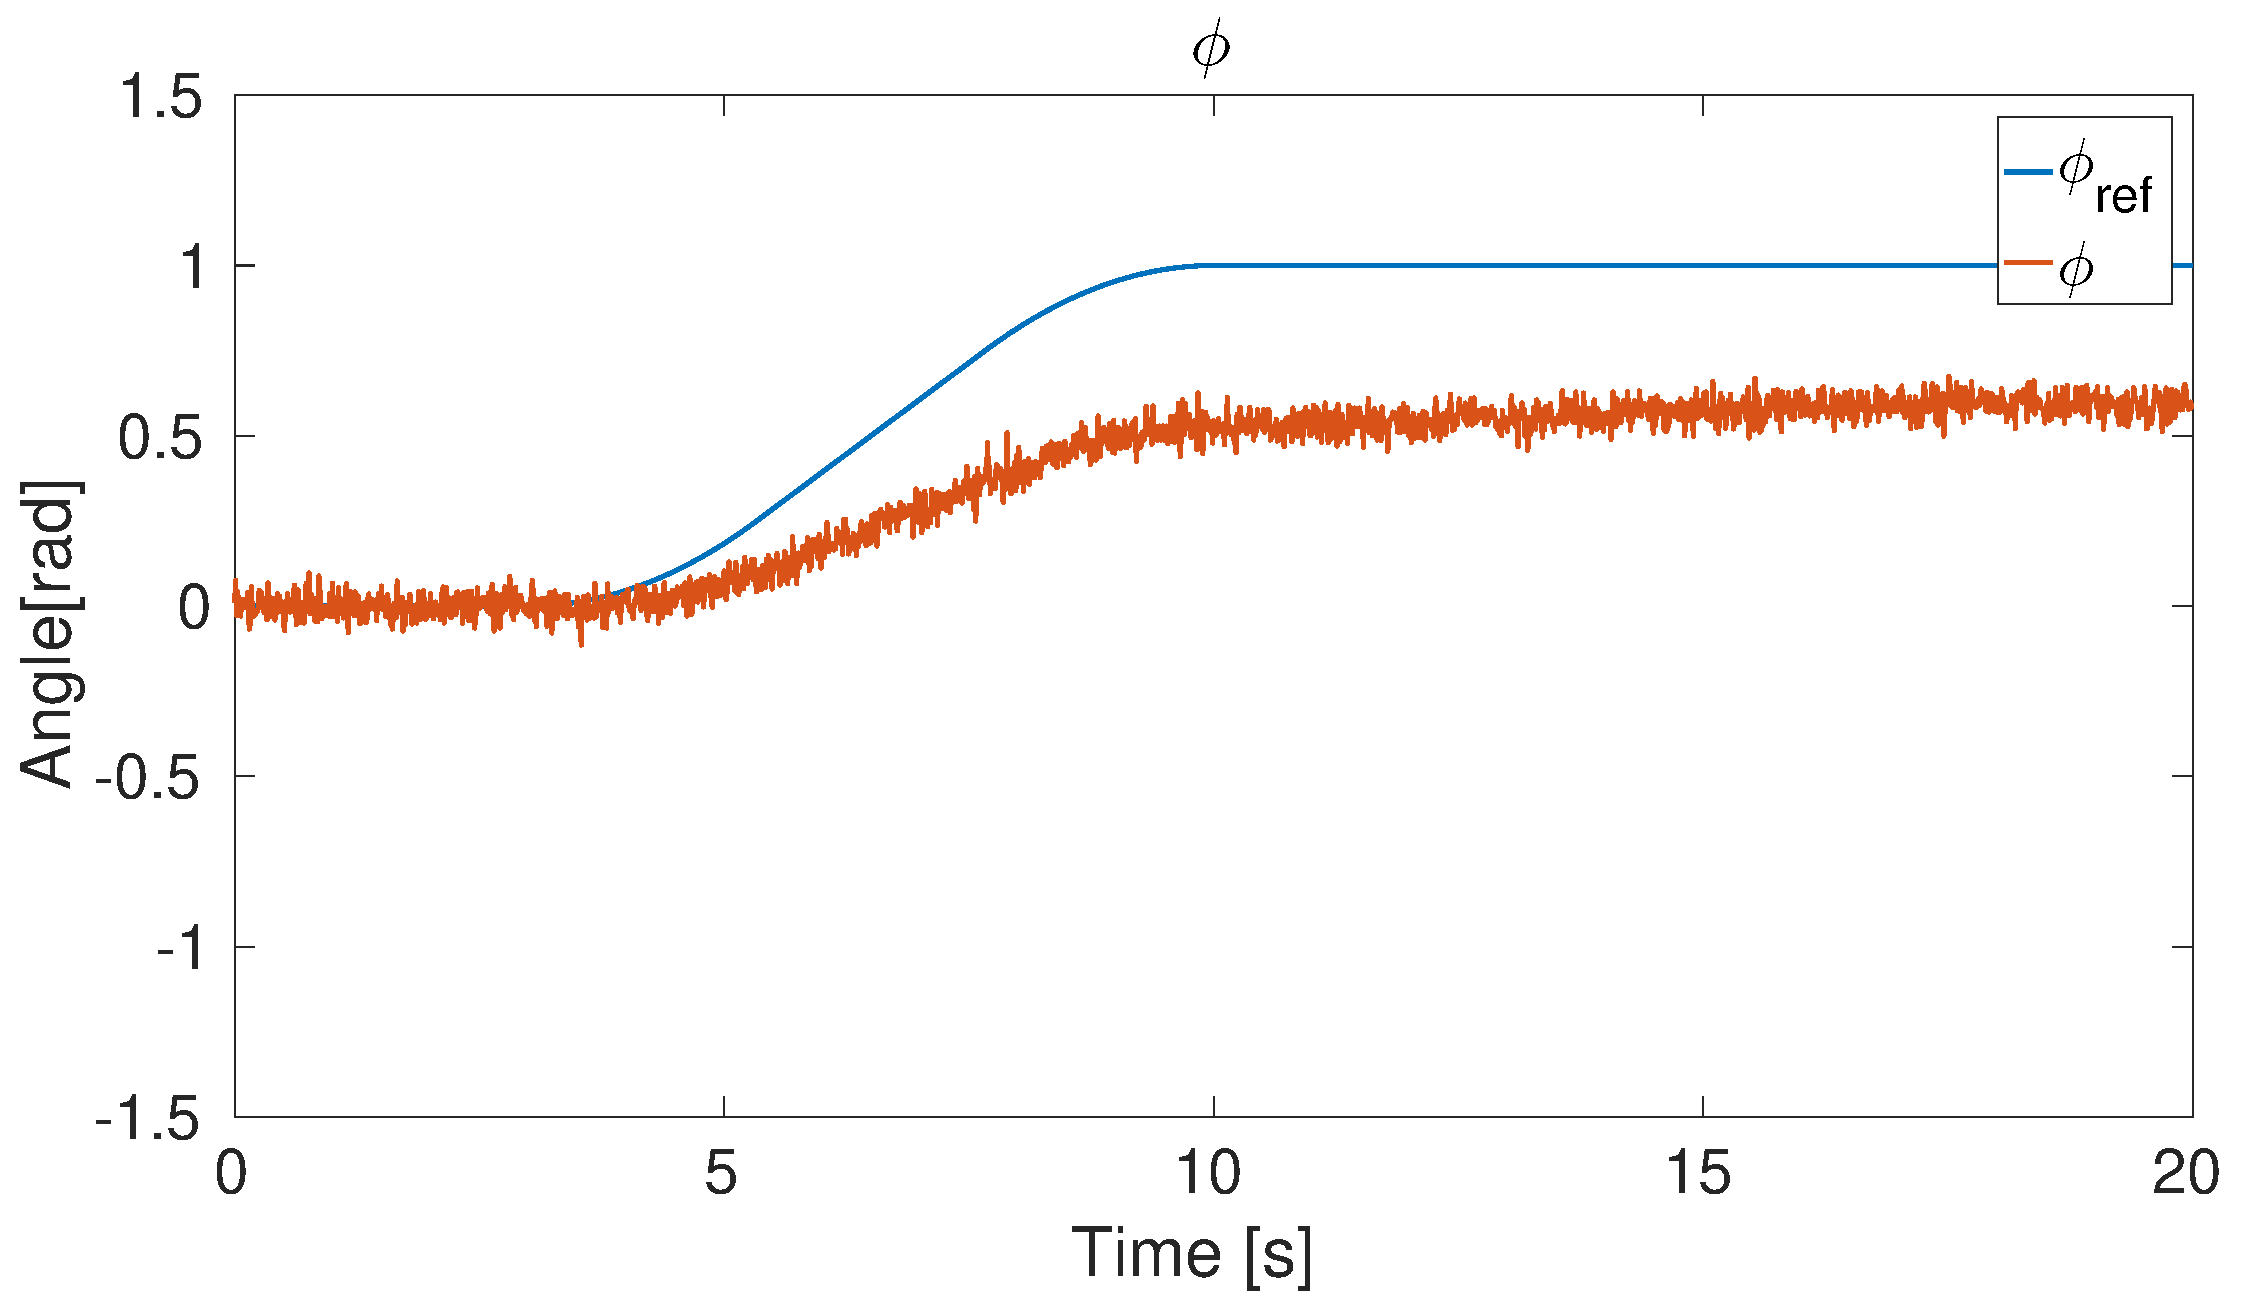
\includegraphics[width=0.4\textwidth]{simStepThetaPhiPhis3e10a1}}
  \qquad
  \subfloat[][\label{fig:testStepPhiTheta05PitchAttitude} A smooth step applied in $\pitchAngle$.]{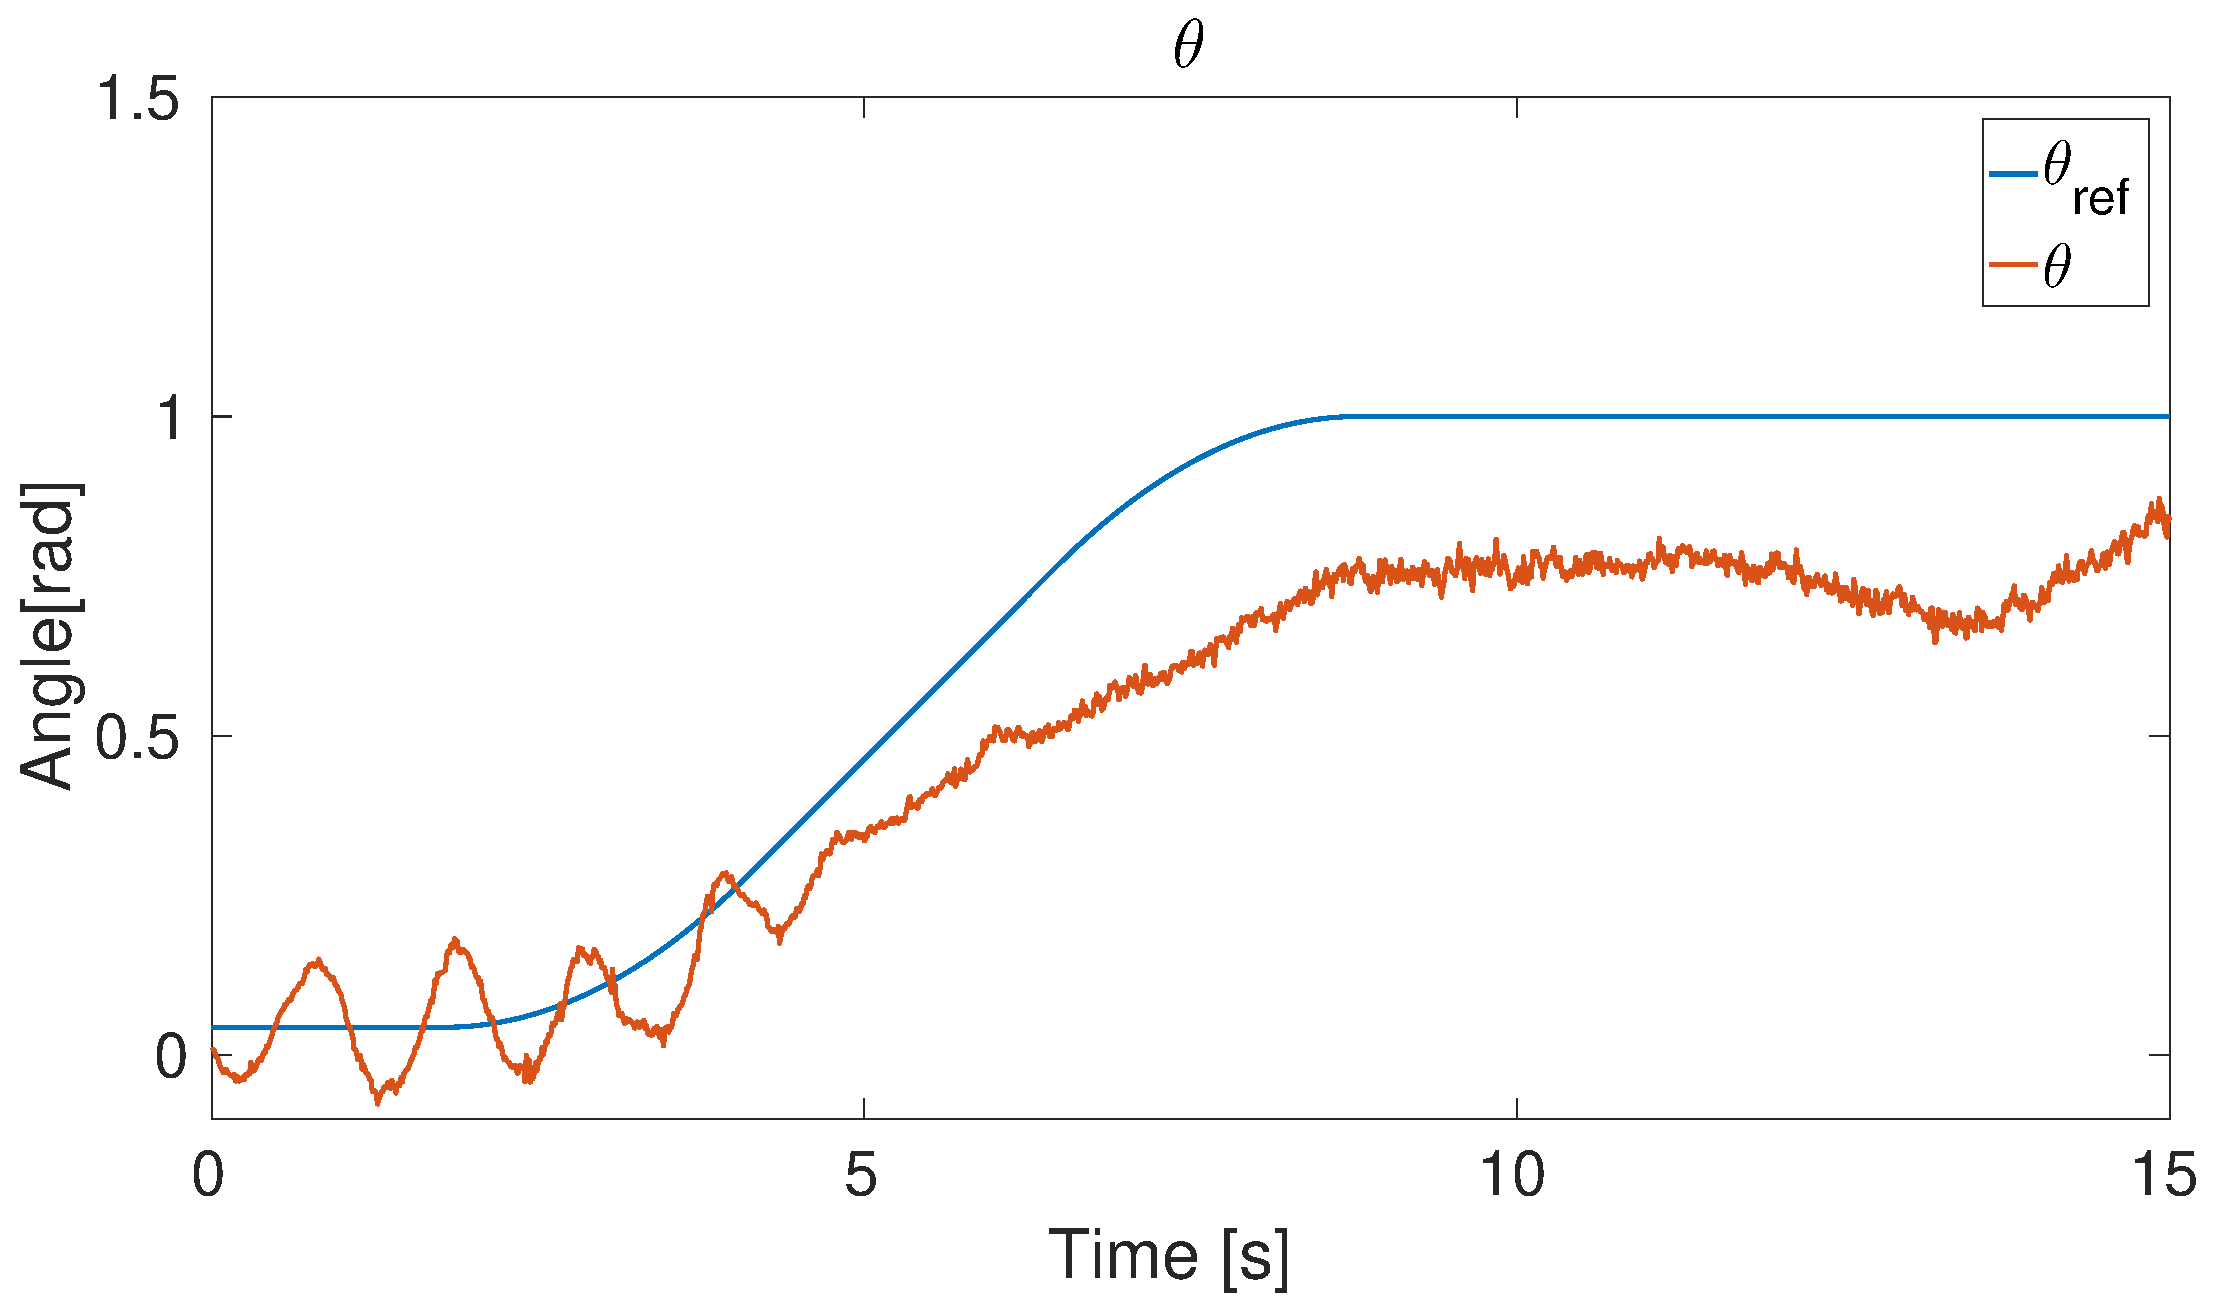
\includegraphics[width=0.4\textwidth]{testStepThetaPhiThetas3e10a1}}
  \qquad
  \subfloat[][\label{fig:simStepPhiTheta05PitchAttitude} A smooth step applied to the simulated \abbrROV in $\pitchAngle$.]{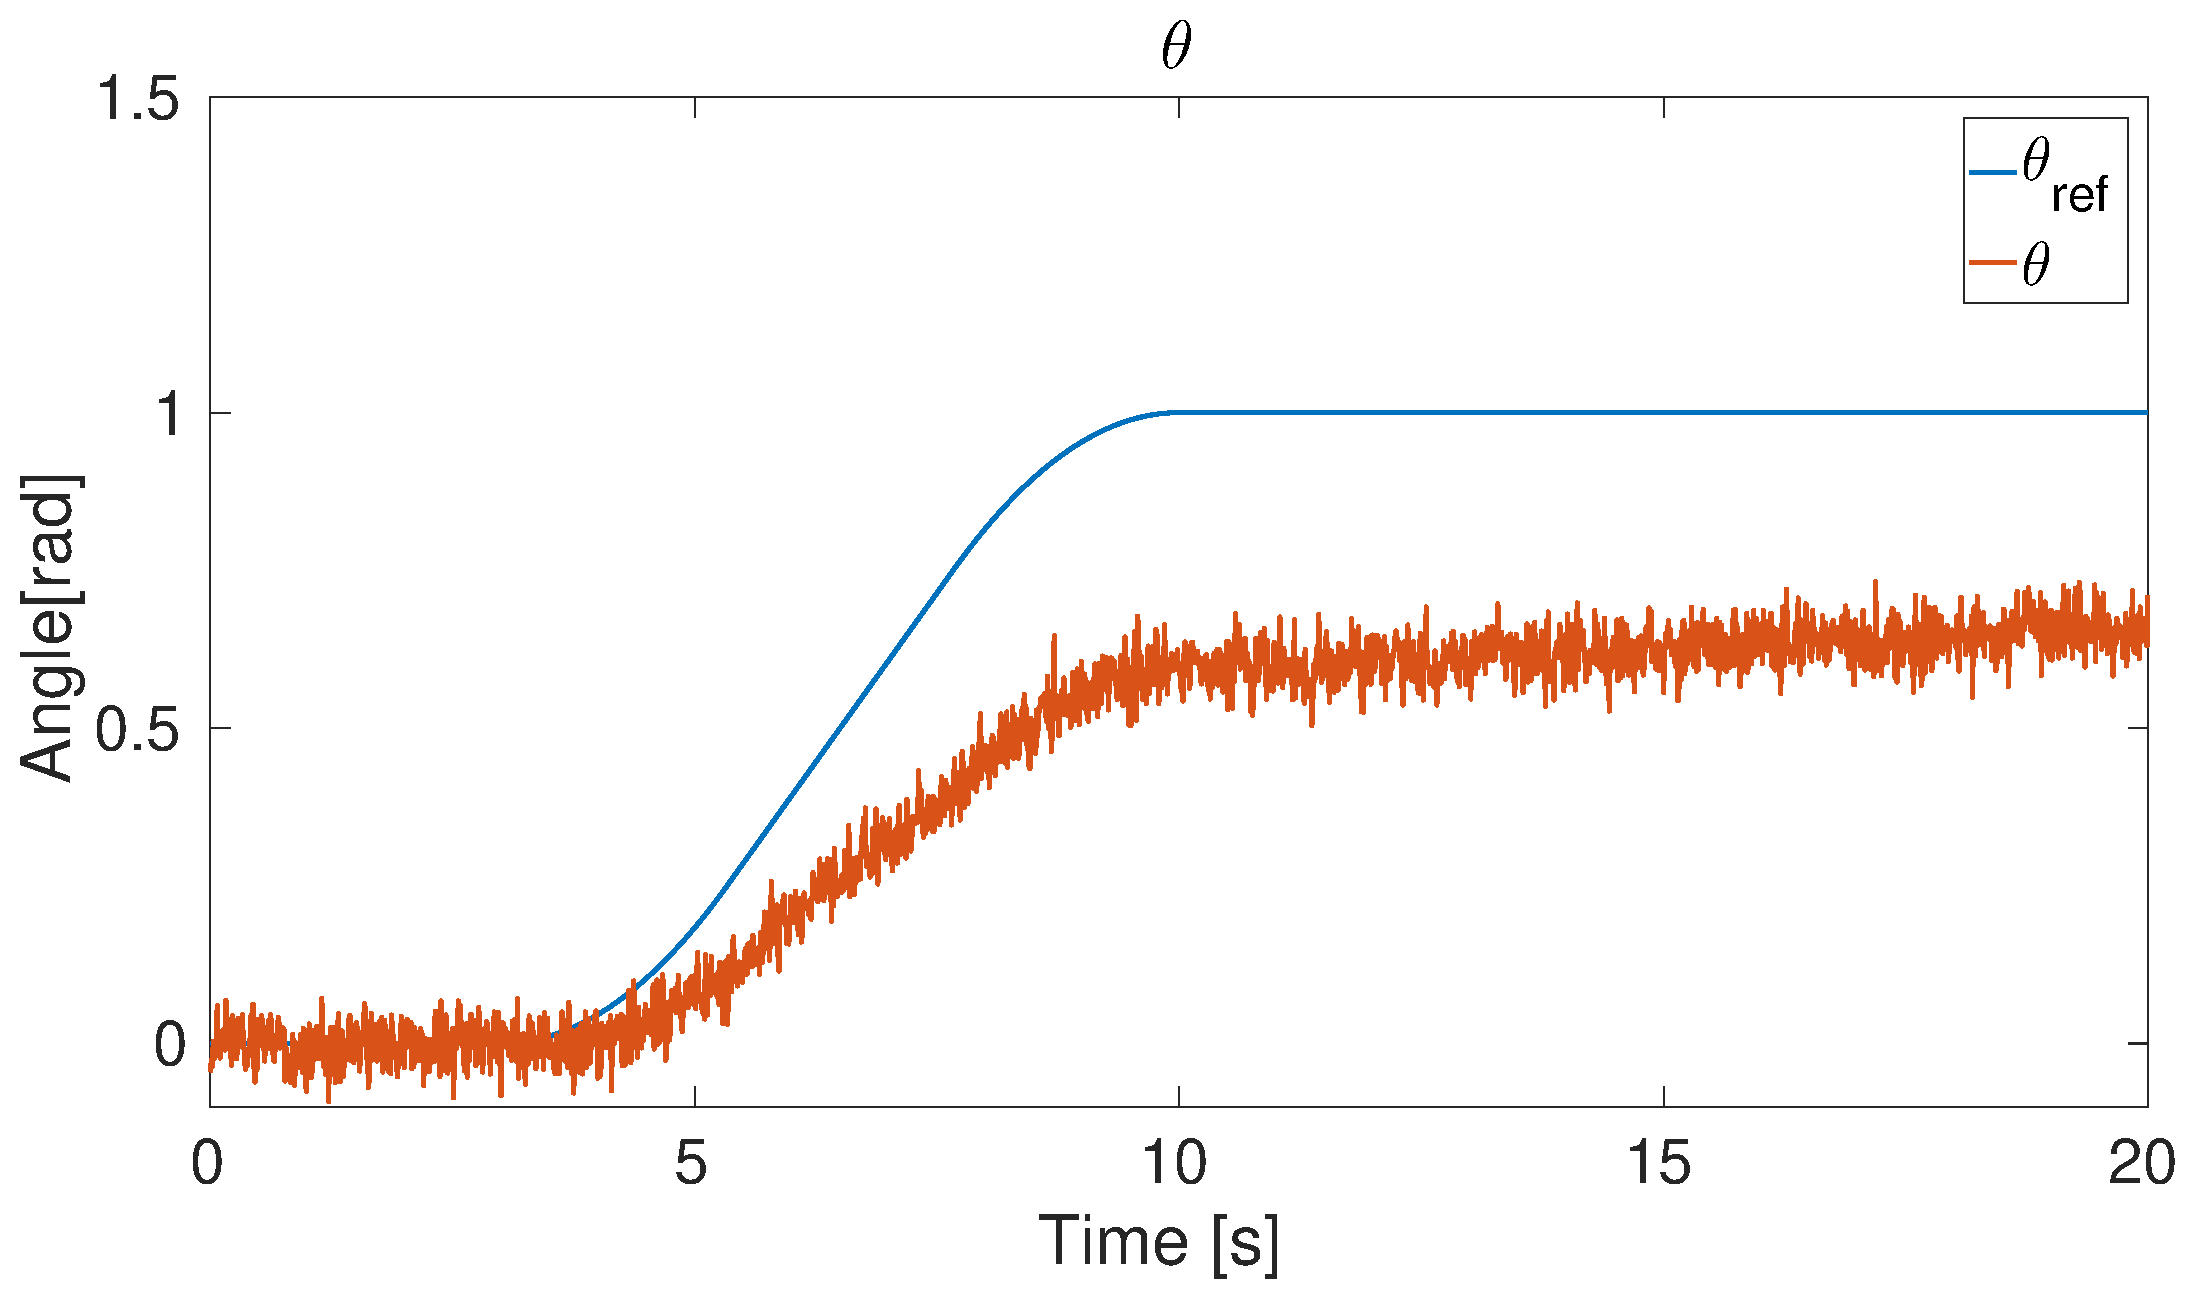
\includegraphics[width=0.4\textwidth]{simStepThetaPhiThetas3e10a1}}
  \caption{\label{fig:StepPhiThetaAttitude}%
  Smooth steps were applied in \pitchAngle and \rollAngle at the same time while using the attitude controller. The attitude angle $\yawAngle$ was kept free during the test.}
\end{figure}

A smoothed step in $\rollAngle$ and $\pitchAngle$ can be seen in \Figureref{fig:StepPhiThetaAttitude}. During the test was the attitude angle $\yawAngle$ kept free. Both $\rollAngle$ and $\pitchAngle$ followed the reference signal well did not reach the reference angle. The steady state error for $\rollAngle$ and $\pitchAngle$ was approximately $0.35$. The simulated results in $\rollAngle$ and $\pitchAngle$ were worse than the real test. The attitude $\rollAngle$ had a steady state error 0.5 and the steady state error for $\pitchAngle$ was 0.4.

%%%%%%%%%%%%%%%%%%%%%%%%%%%Rate%%%%%%%%%%%%%%%%
\begin{figure}
\centering
  \subfloat[][\label{fig:testStepAllPRate} A smooth step applied in $\rollVelocity$.]{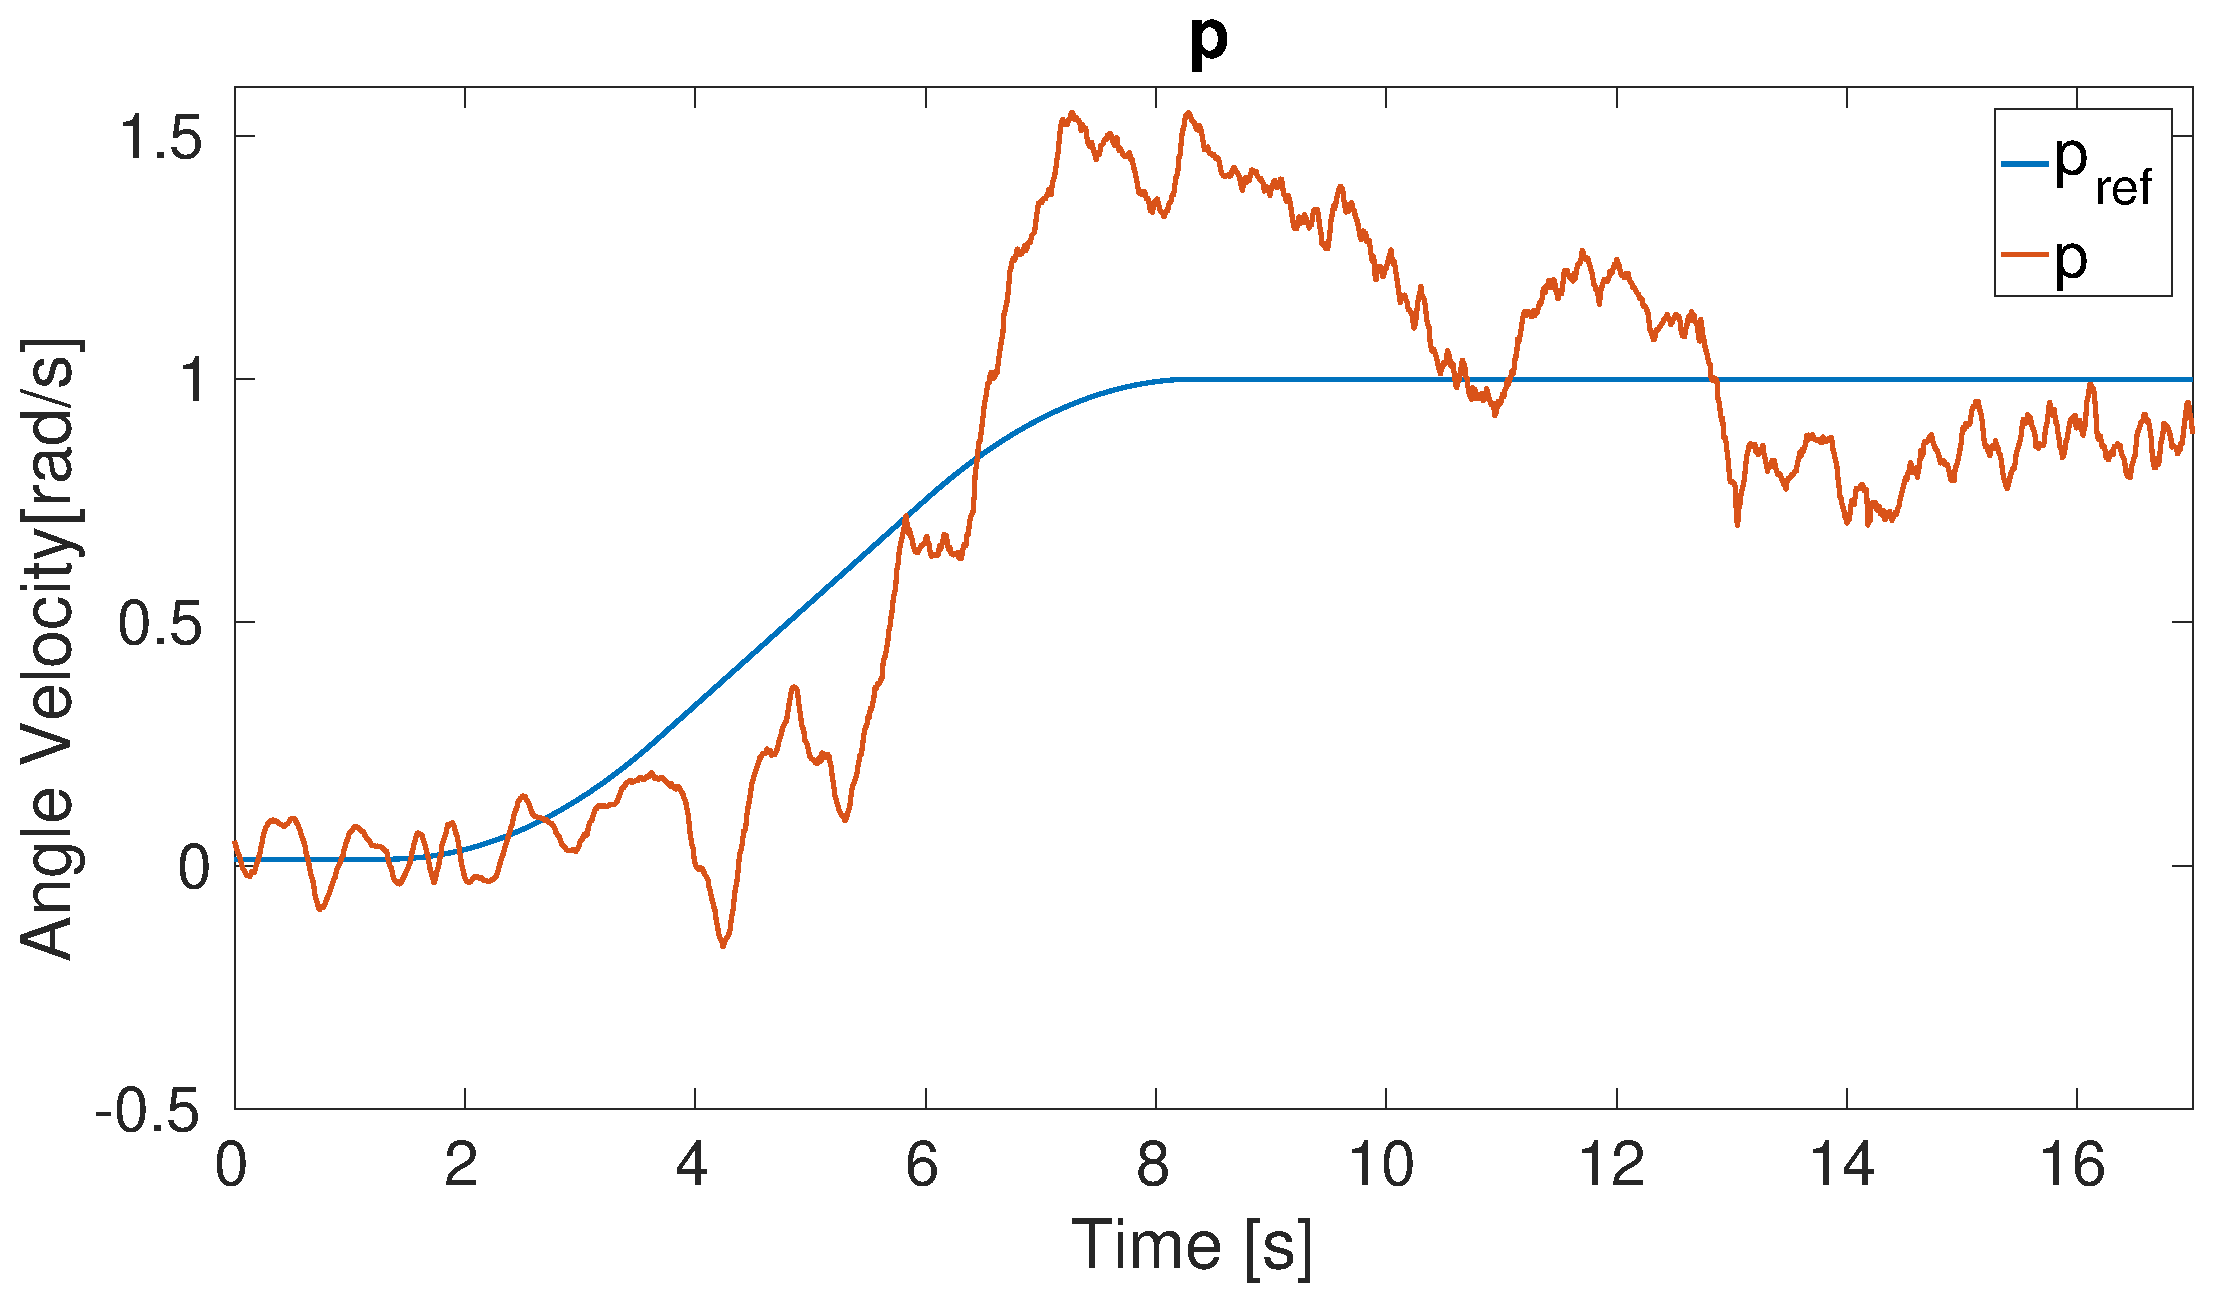
\includegraphics[width=0.4\textwidth]{testStepAllPs3e10a1}}
  \qquad
  \subfloat[][\label{fig:simStepAllPRate} A step applied to the simulated \abbrROV in $\rollVelocity$.]{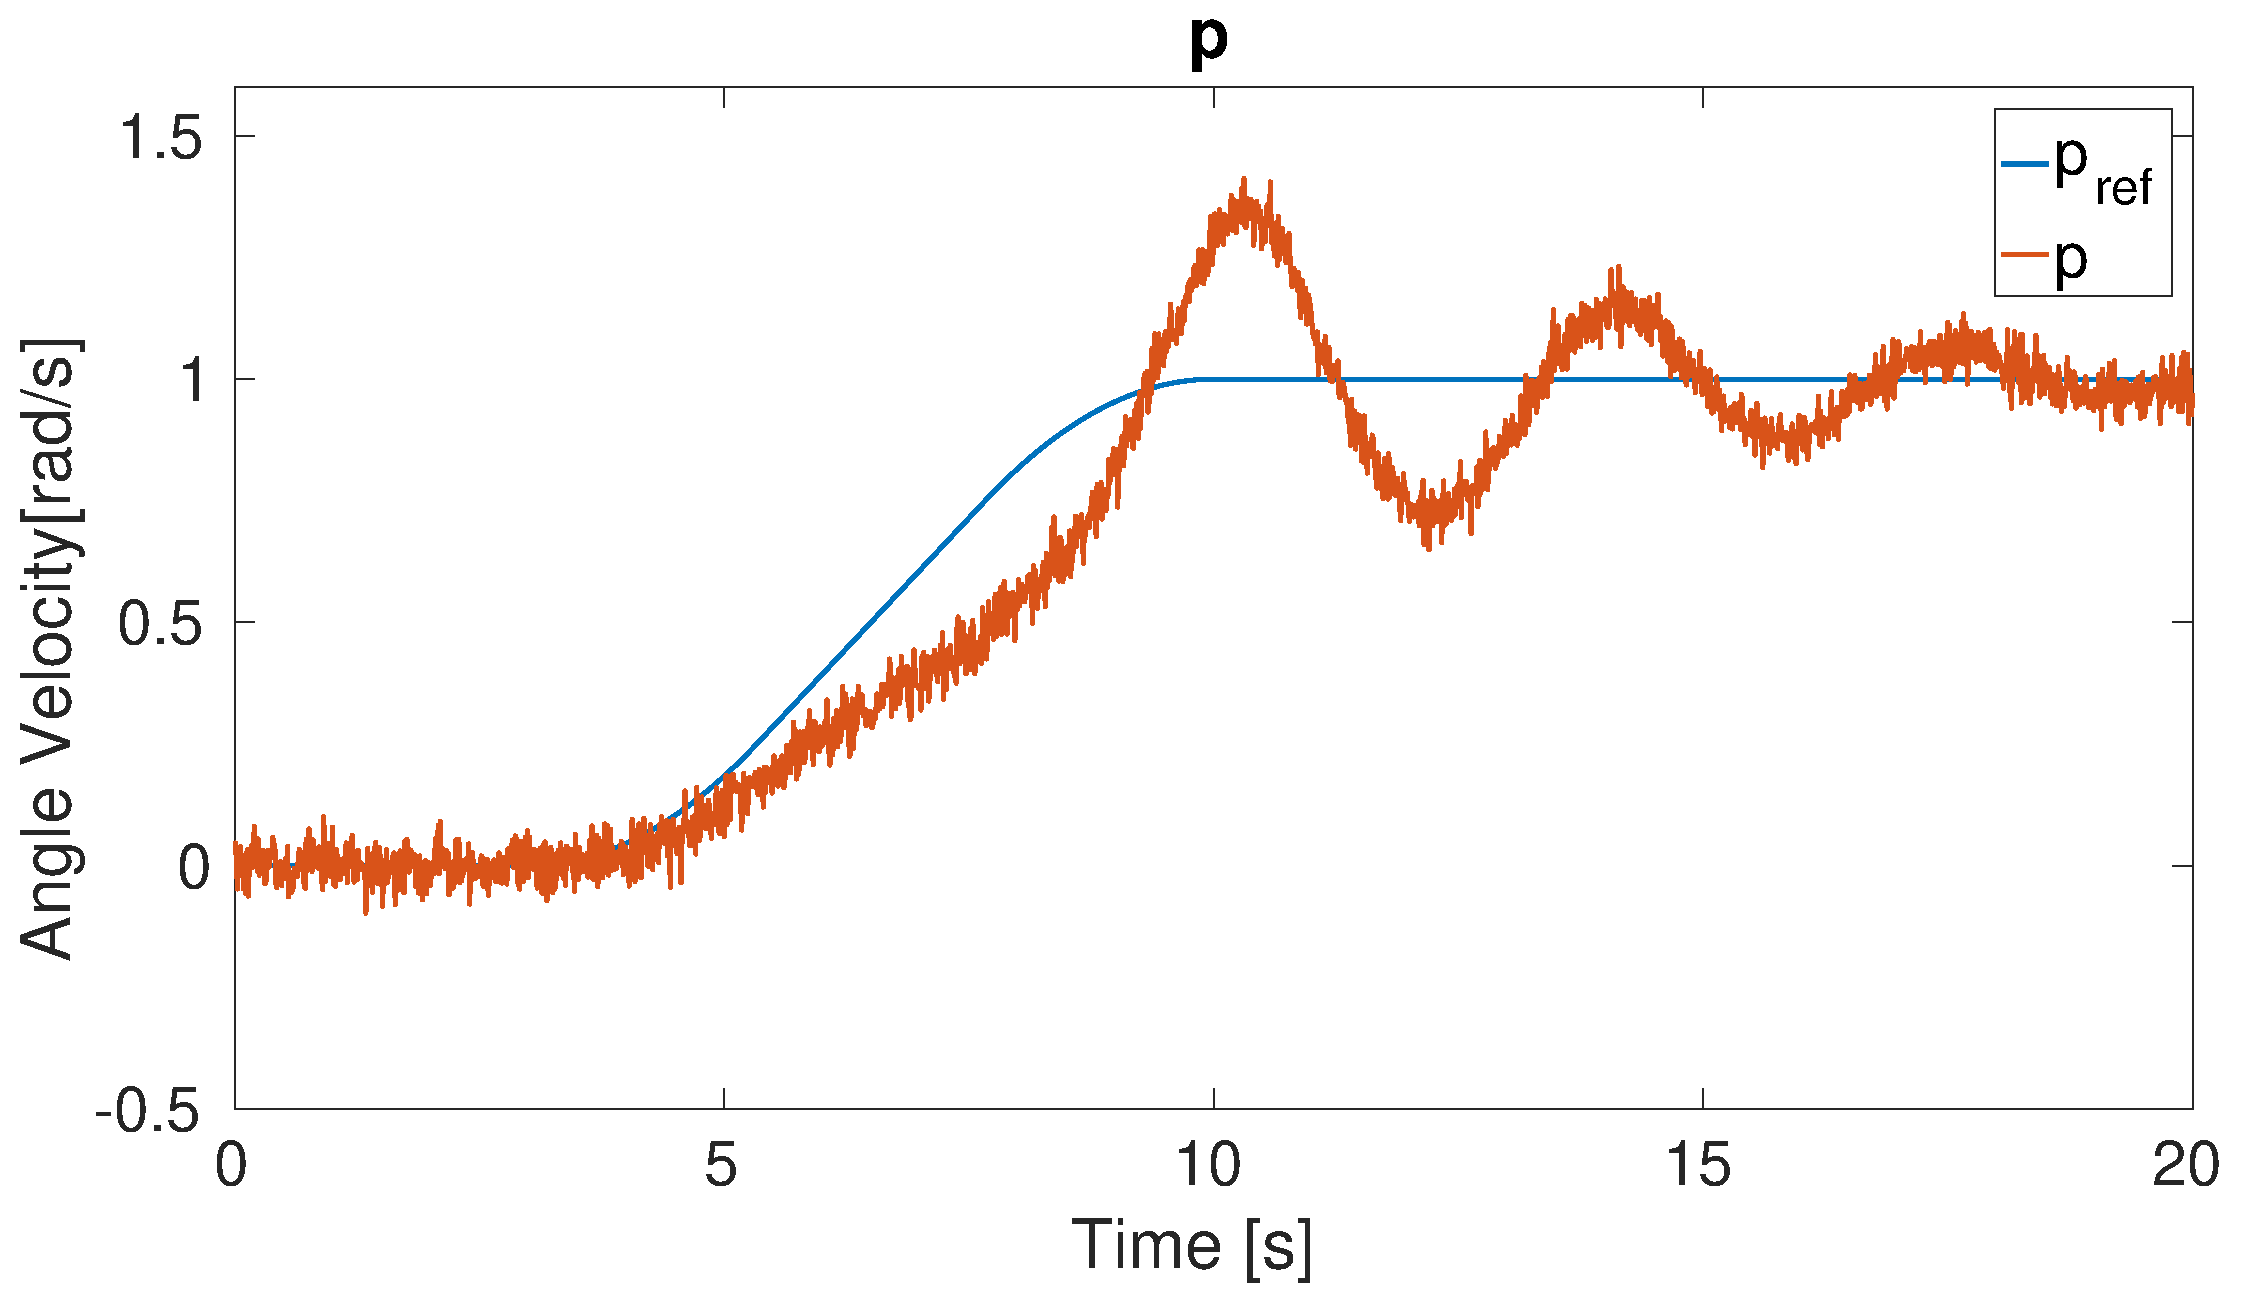
\includegraphics[width=0.4\textwidth]{simStepAllPs3e10a1}}
  \qquad
  \subfloat[][\label{fig:testStepAllQRate} A smooth step applied in $\pitchVelocity$.]{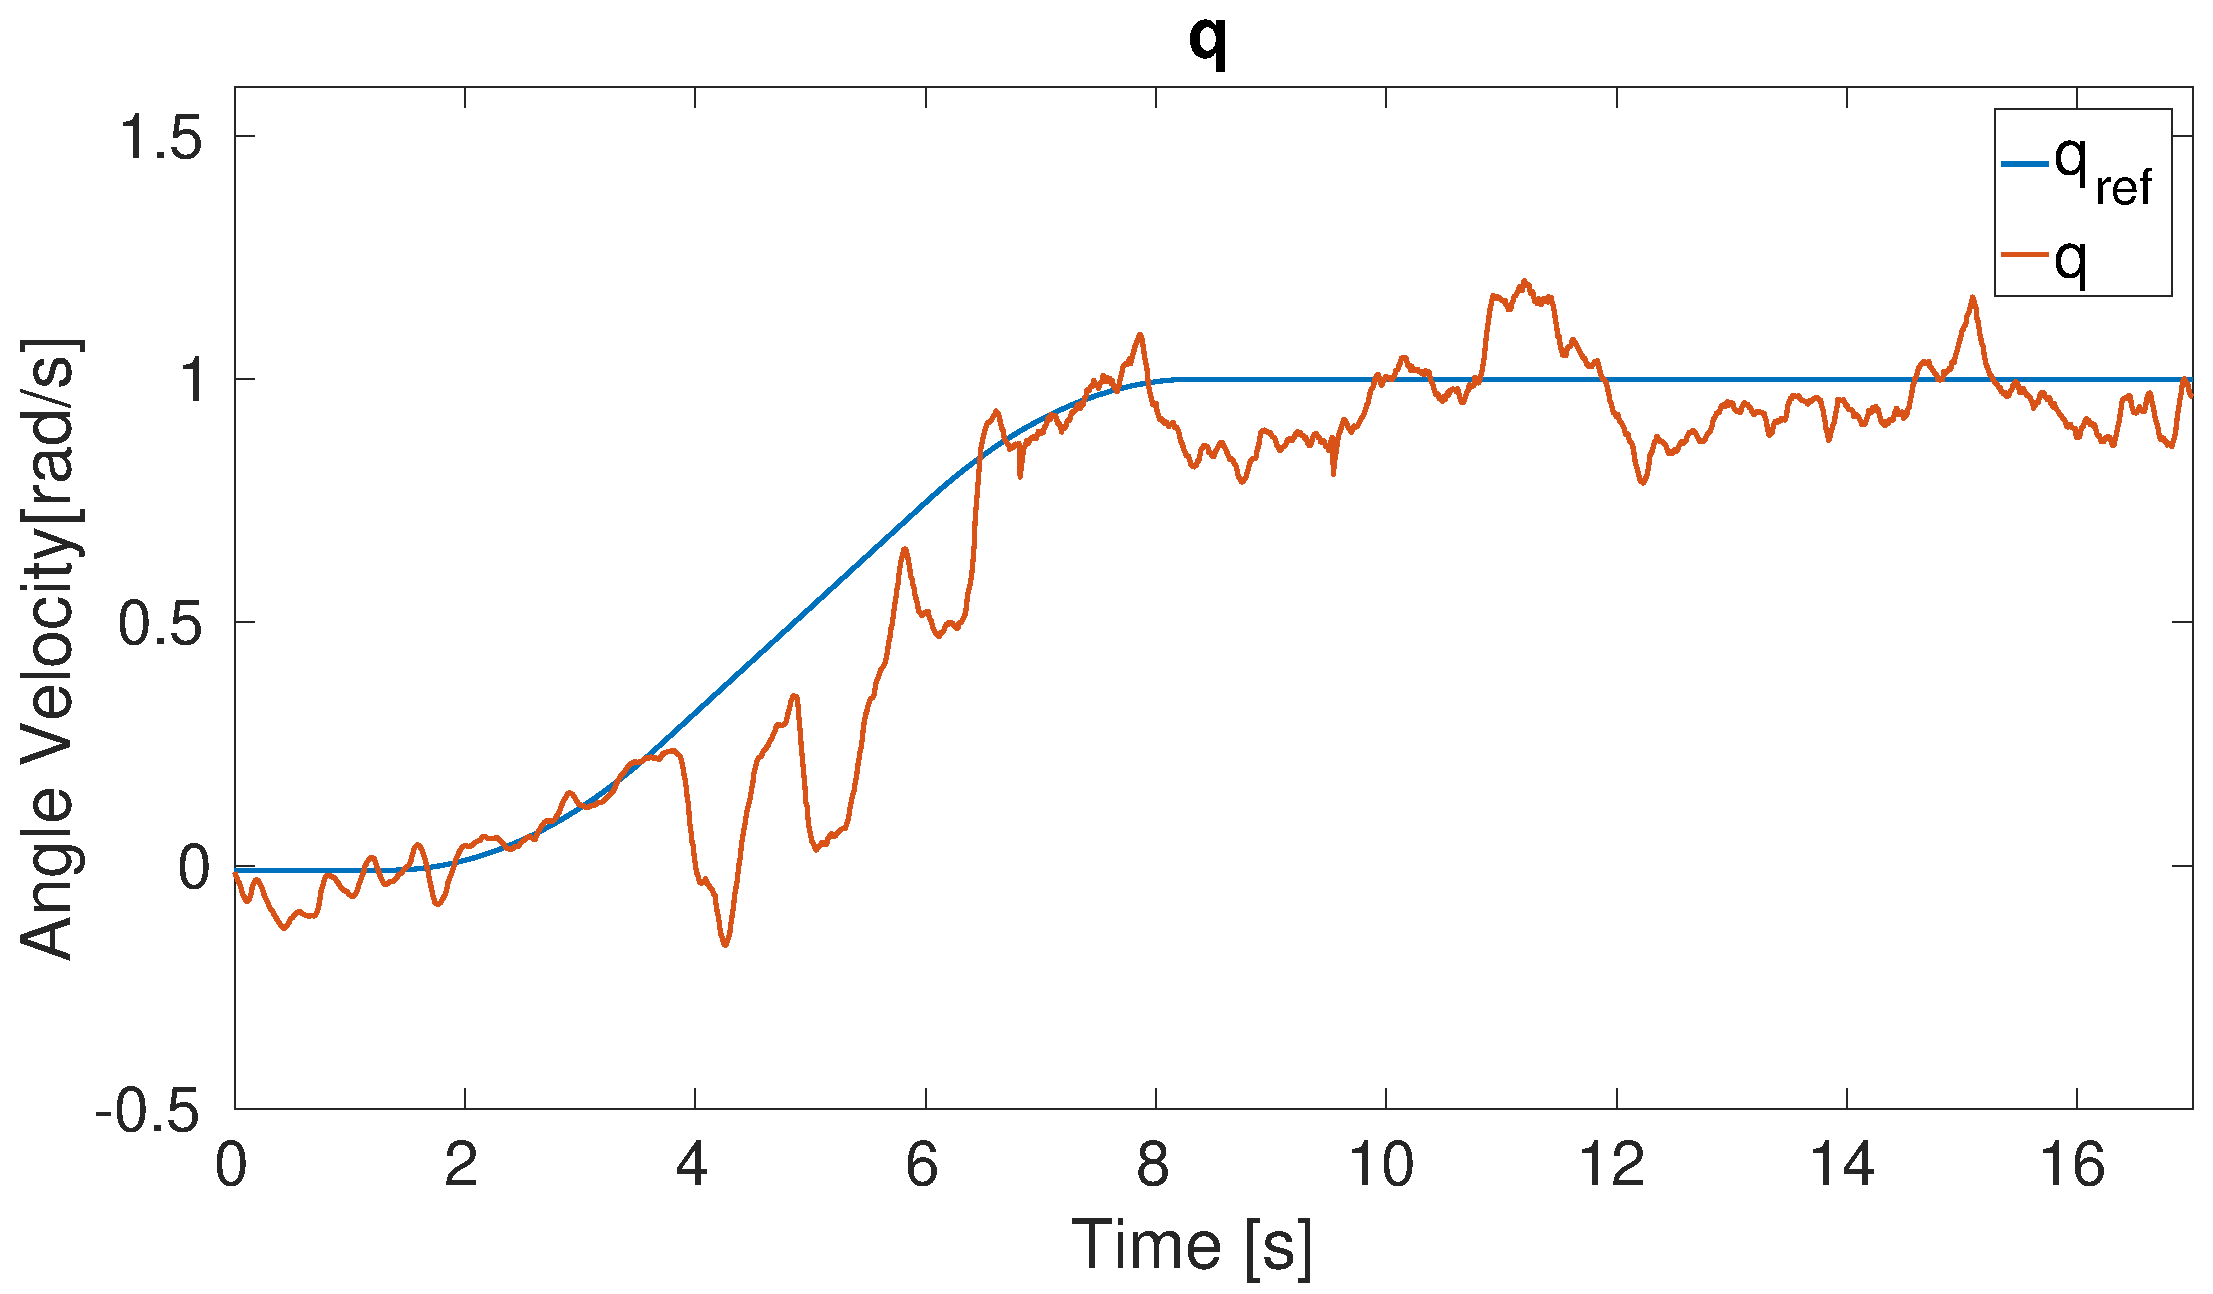
\includegraphics[width=0.4\textwidth]{testStepAllQs3e10a1}}
  \qquad
  \subfloat[][\label{fig:simStepAllQRate} A step applied to the simulated \abbrROV in $\pitchVelocity$.]{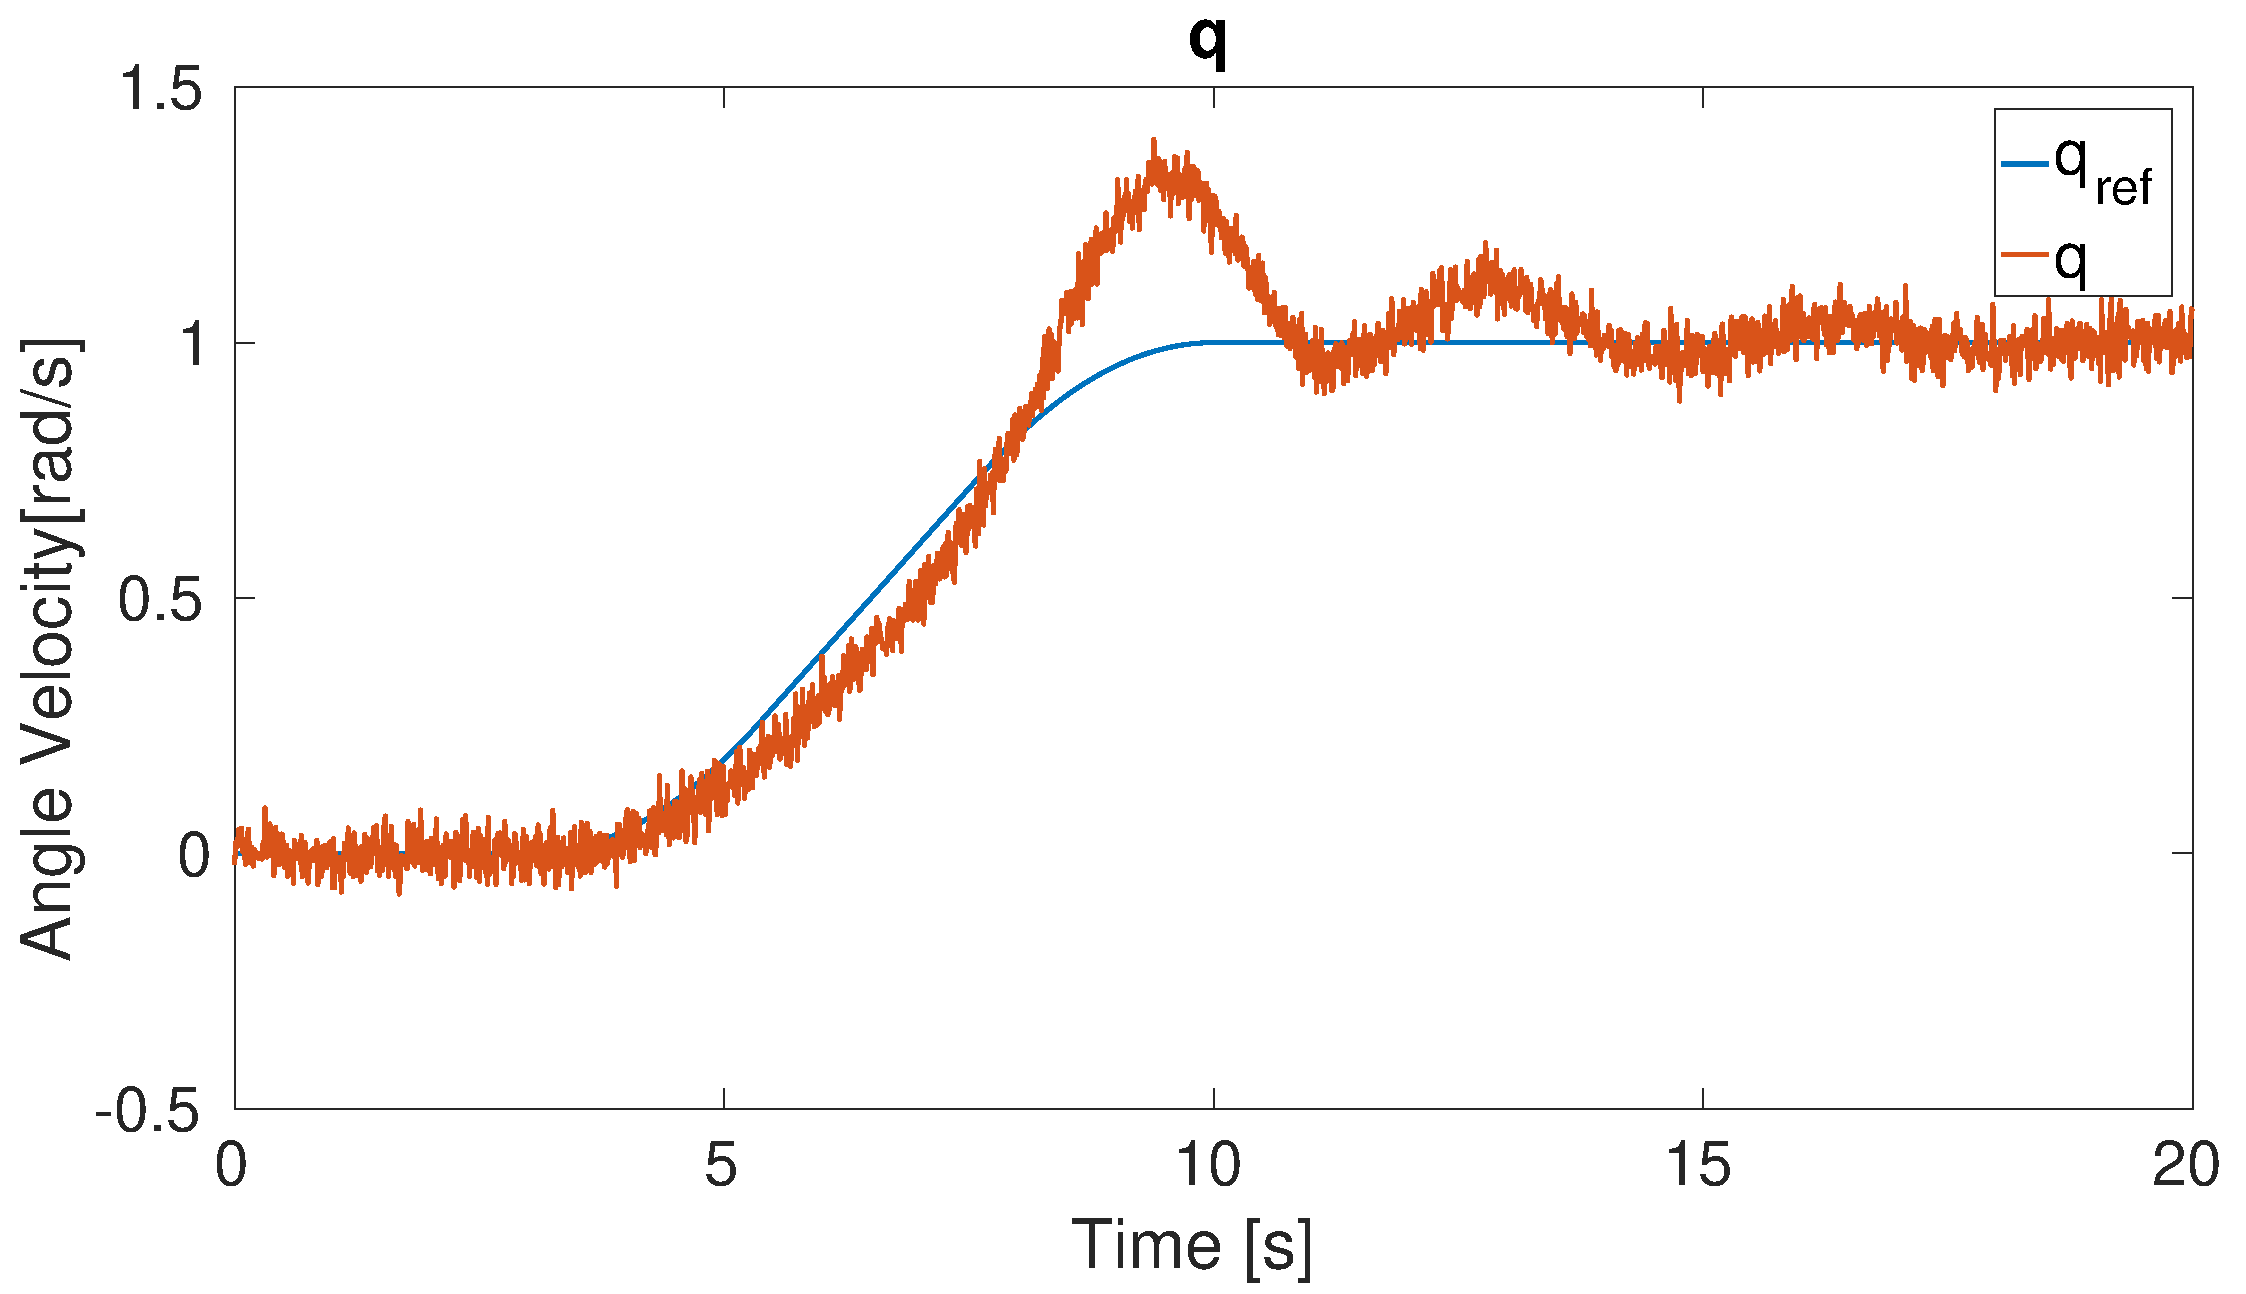
\includegraphics[width=0.4\textwidth]{simStepAllQs3e10a1}}
  \qquad
  \subfloat[][\label{fig:testStepAllRRate} A smooth step applied in $\yawVelocity$.]{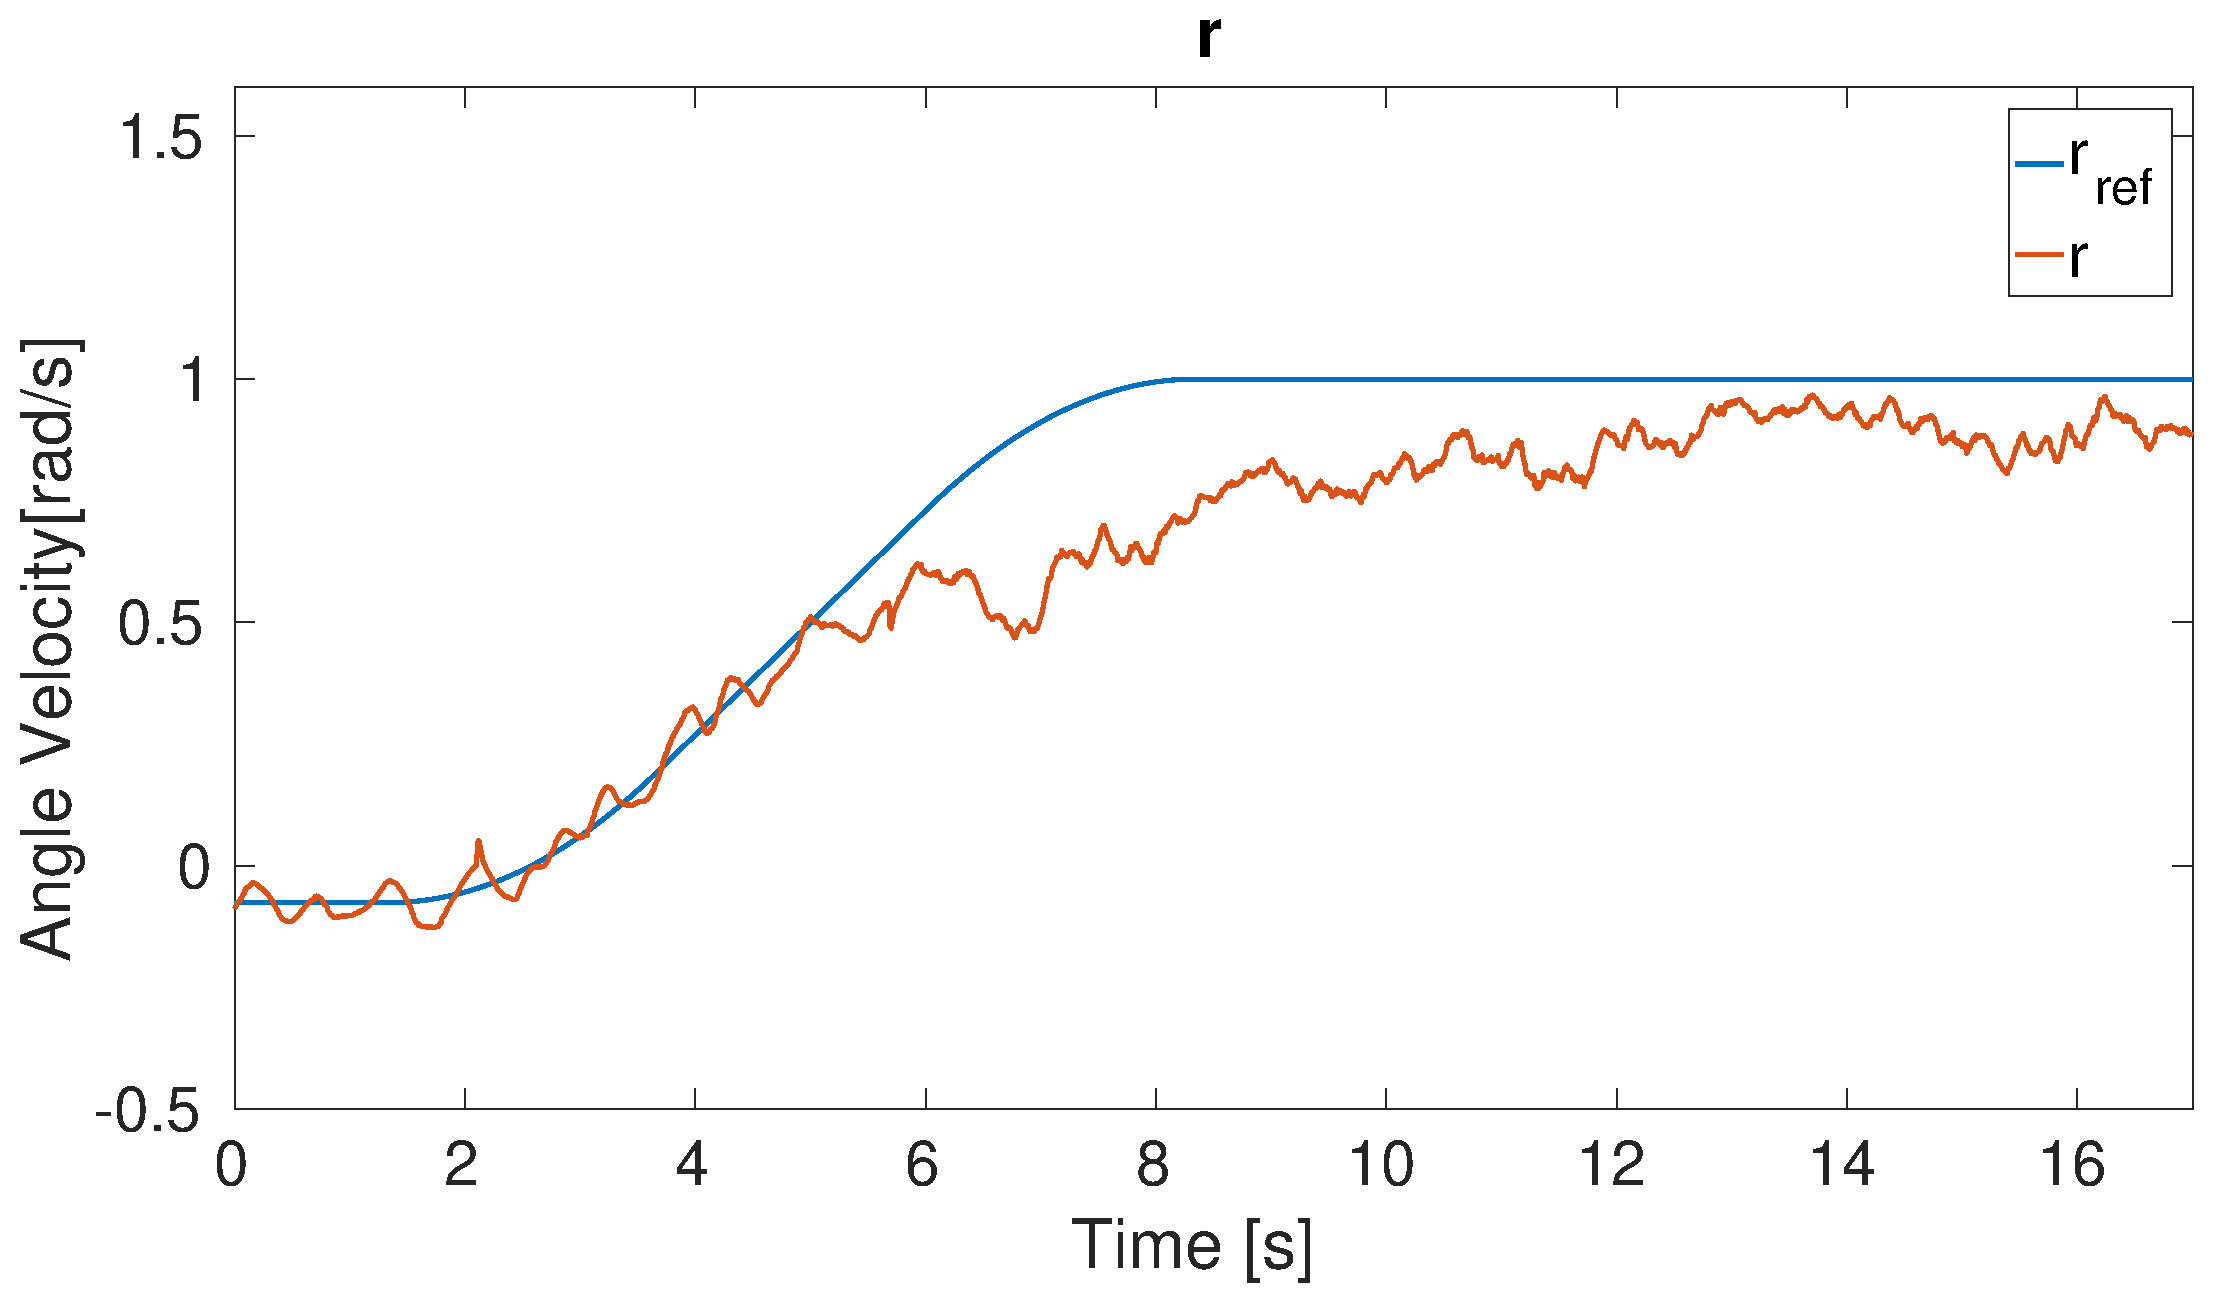
\includegraphics[width=0.4\textwidth]{testStepAllRs3e10a1}}
  \qquad
  \subfloat[][\label{fig:simStepAllRRate} A step applied to the simulated \abbrROV in $\yawVelocity$.]{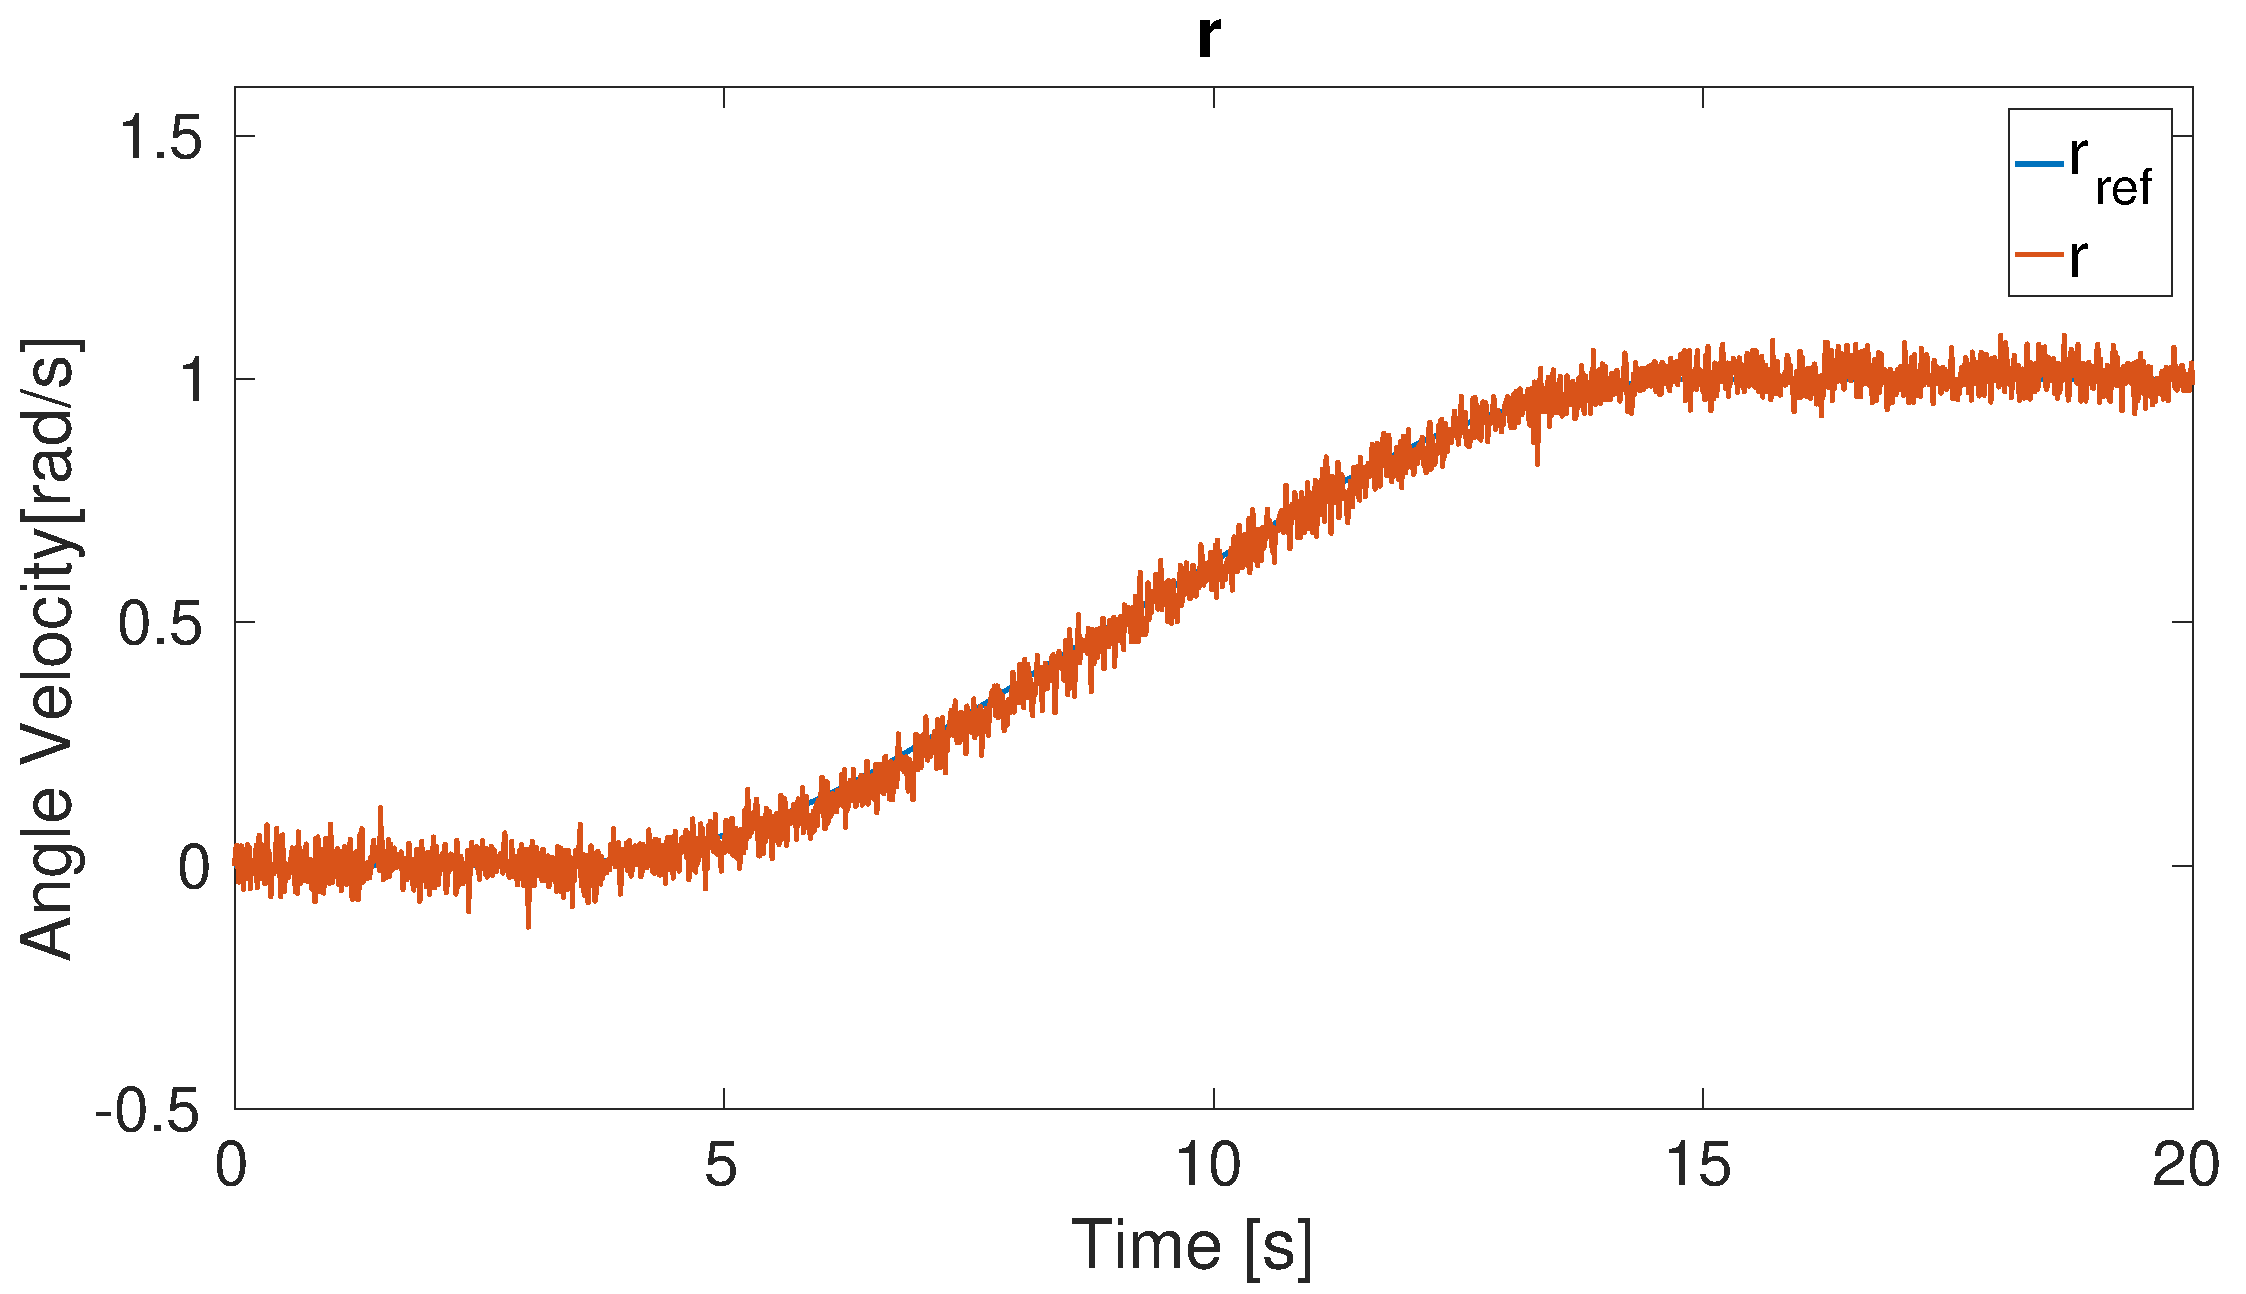
\includegraphics[width=0.4\textwidth]{simStepAllRs3e10a1}}
  \caption{\label{fig:StepAllRate}% 
  Smooth steps were applied in all angular velocities at the same time while using the rate controller.}
\end{figure}

\Figureref{fig:StepAllRate} shows a smooth step applied in all angular velocities while using the rate controller. An overshoot of 0.5 is achieved in $\rollVelocity$ for the real test while in the simulation only has an overshoot of 0.2. Both the real test and the simulation in $\rollVelocity$ followed the reference signal well and had a small steady state error. The real and simulated test followed the reference value well in $\pitchVelocity$ and had negligible steady state errors. However, had the real test no overshoot while the simulation in $\pitchVelocity$ had an overshoot of 0.4. The simulated test in $\yawVelocity$ performed really well and almost followed the reference perfectly. The real test in $\yawVelocity$ performed well, but it was slow to rise to the requested reference signal and had a small steady state error of 0.1. 

\begin{figure}
\centering
  \subfloat[][\label{fig:testSinAllPRate} A sine signal with amplitude $1$ and frequency $0.5\hertz$ applied in $\rollVelocity$.]{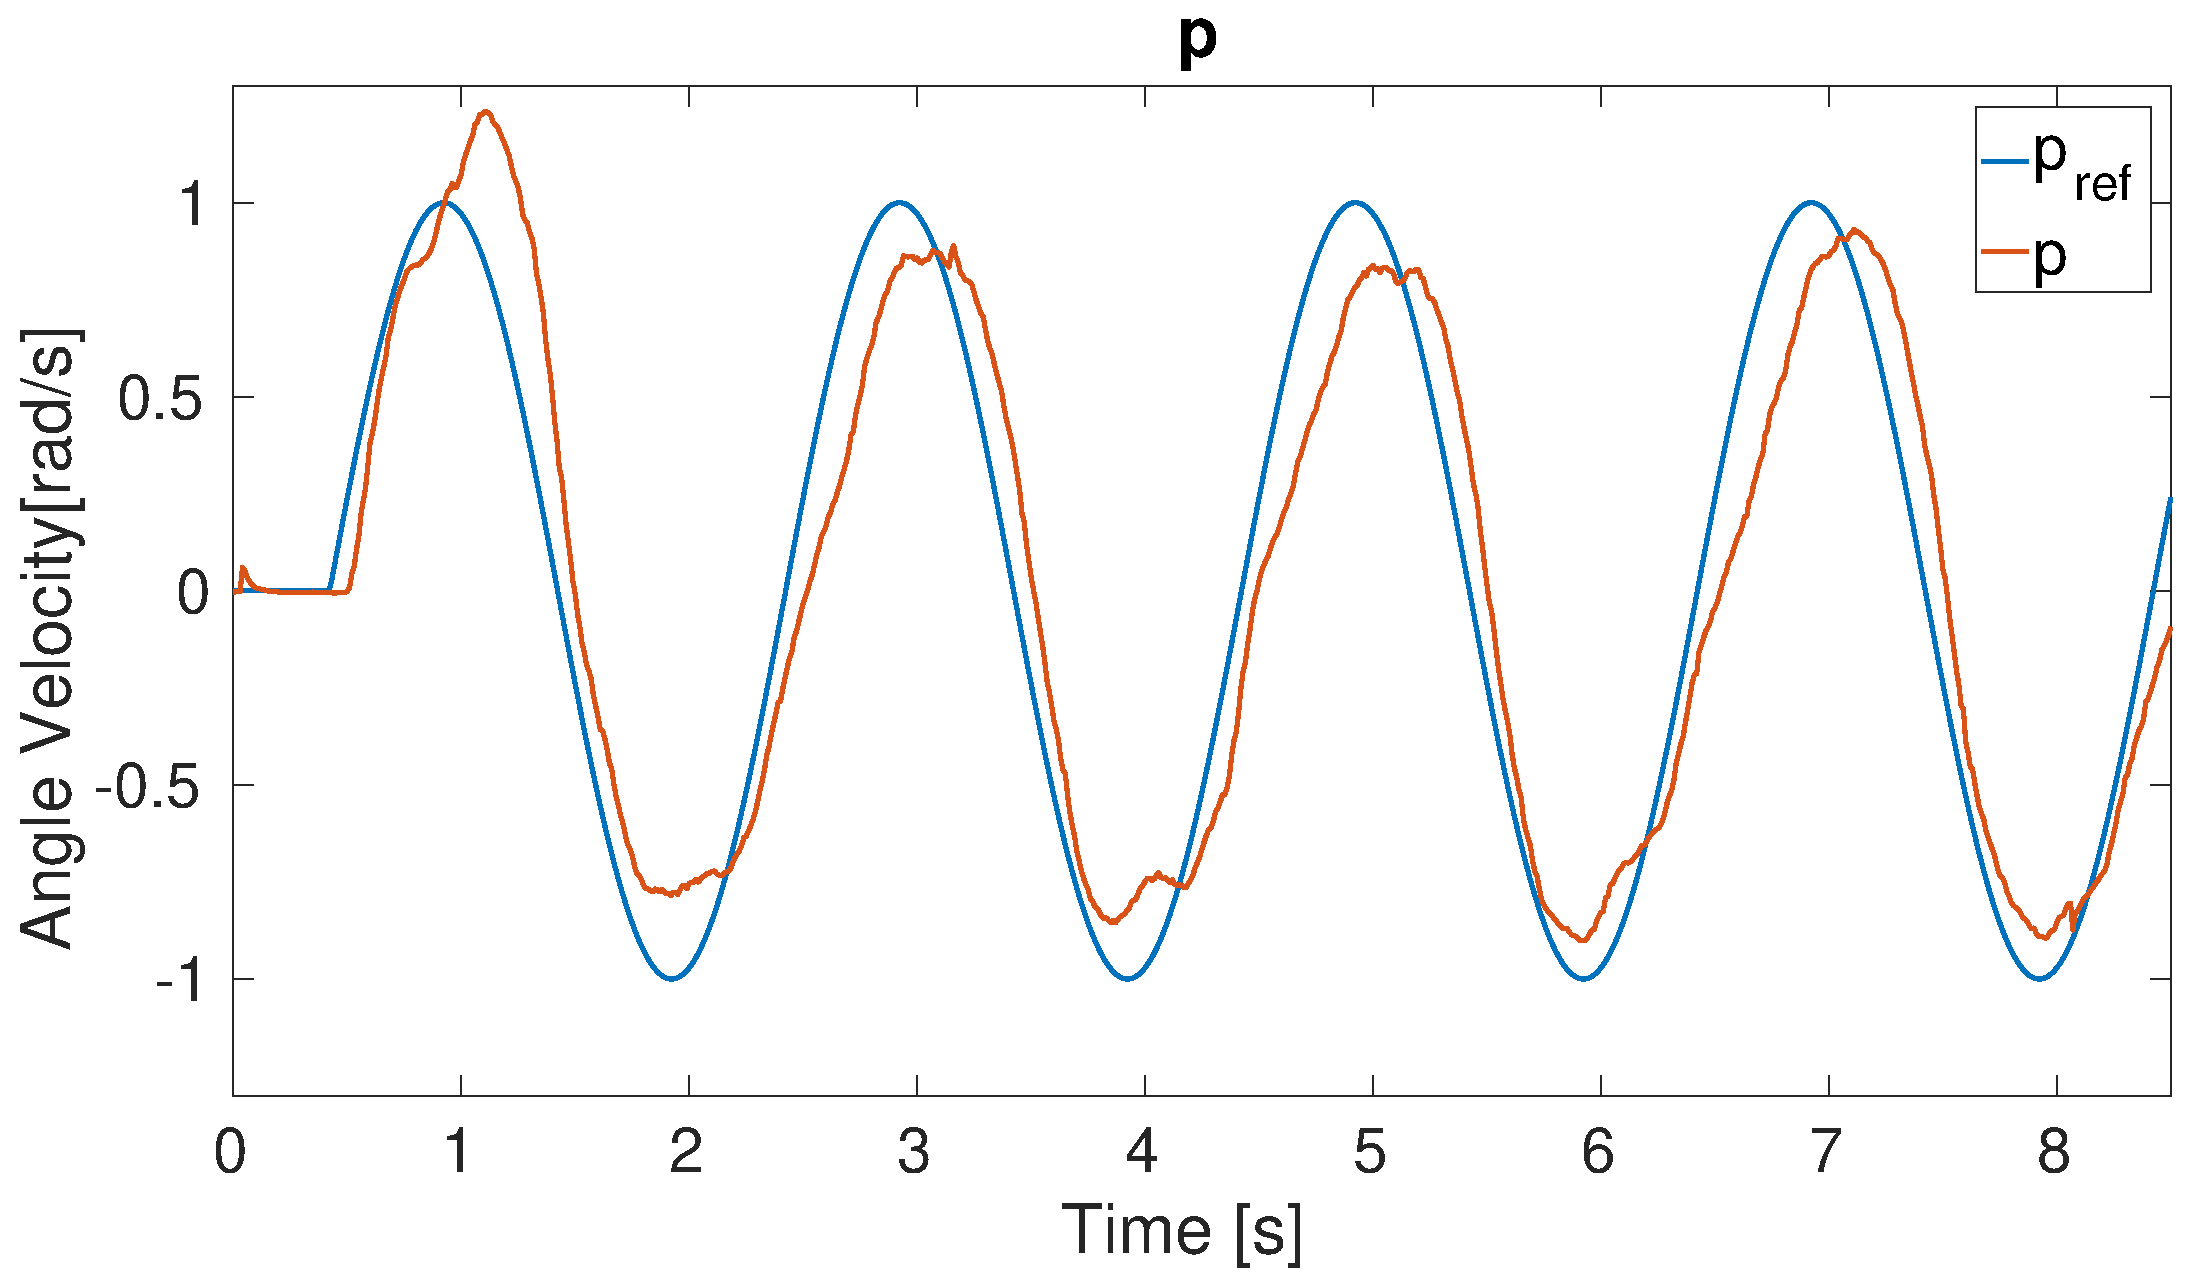
\includegraphics[width=0.4\textwidth]{testSinAllPA1}}
  \qquad
  \subfloat[][\label{fig:simSinAllPRate}A sine signal with amplitude $1$ and frequency $0.5\hertz$ applied to the simulated \abbrROV in $\rollVelocity$.]{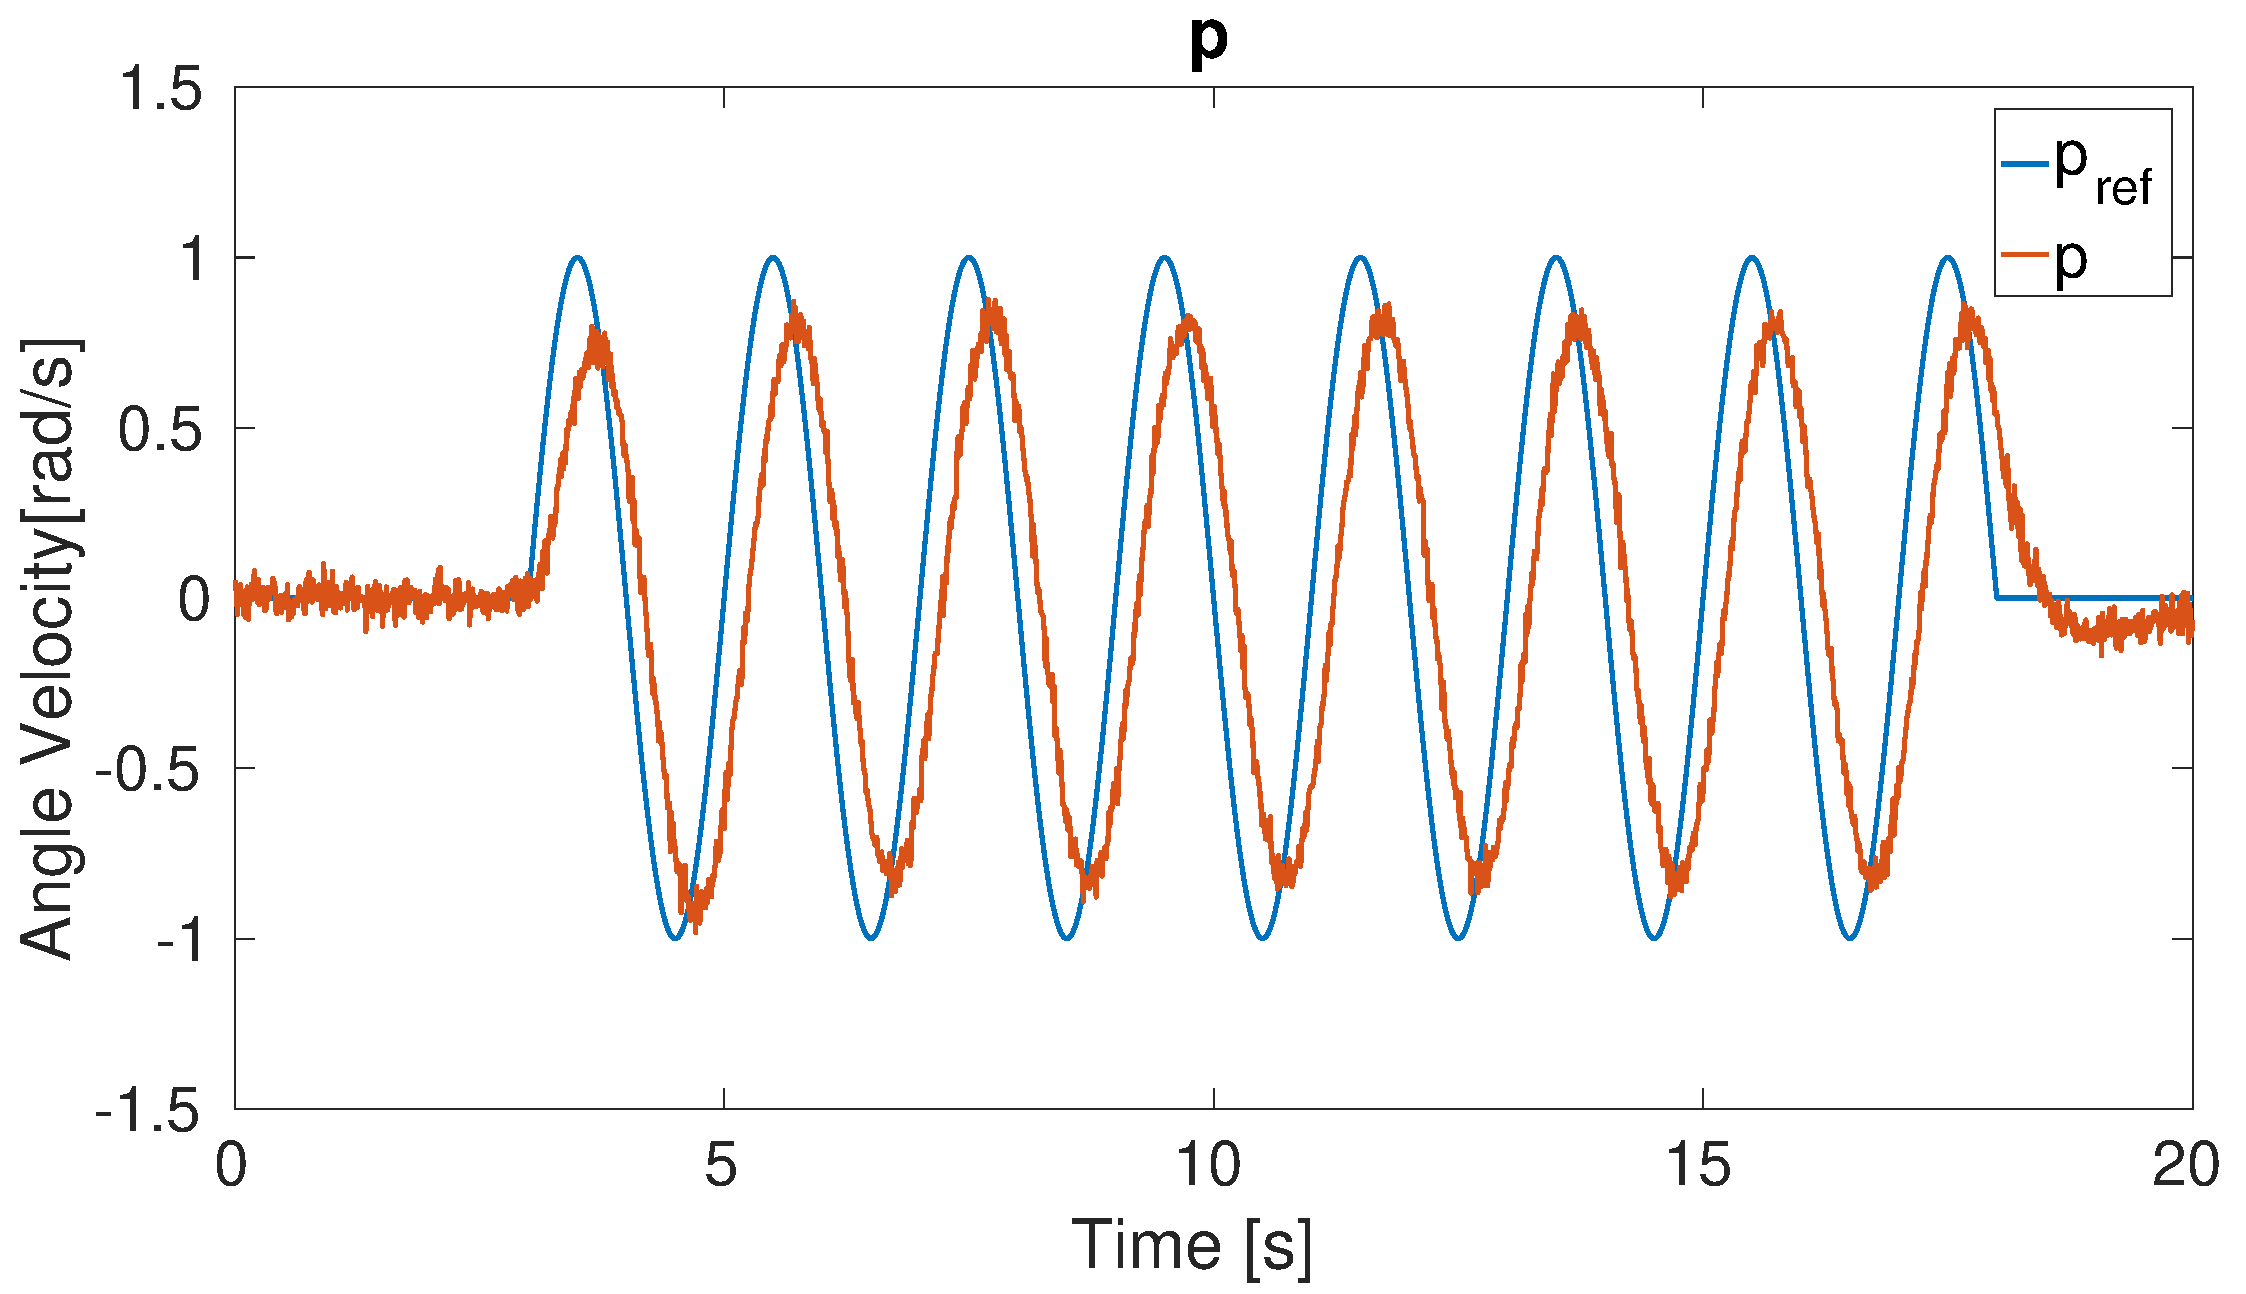
\includegraphics[width=0.4\textwidth]{simSinAllPA1}}
  \qquad
  \subfloat[][\label{fig:testSinAllQRate} A sine signal with amplitude $1$ and frequency $0.5\hertz$ applied in $\pitchVelocity$.]{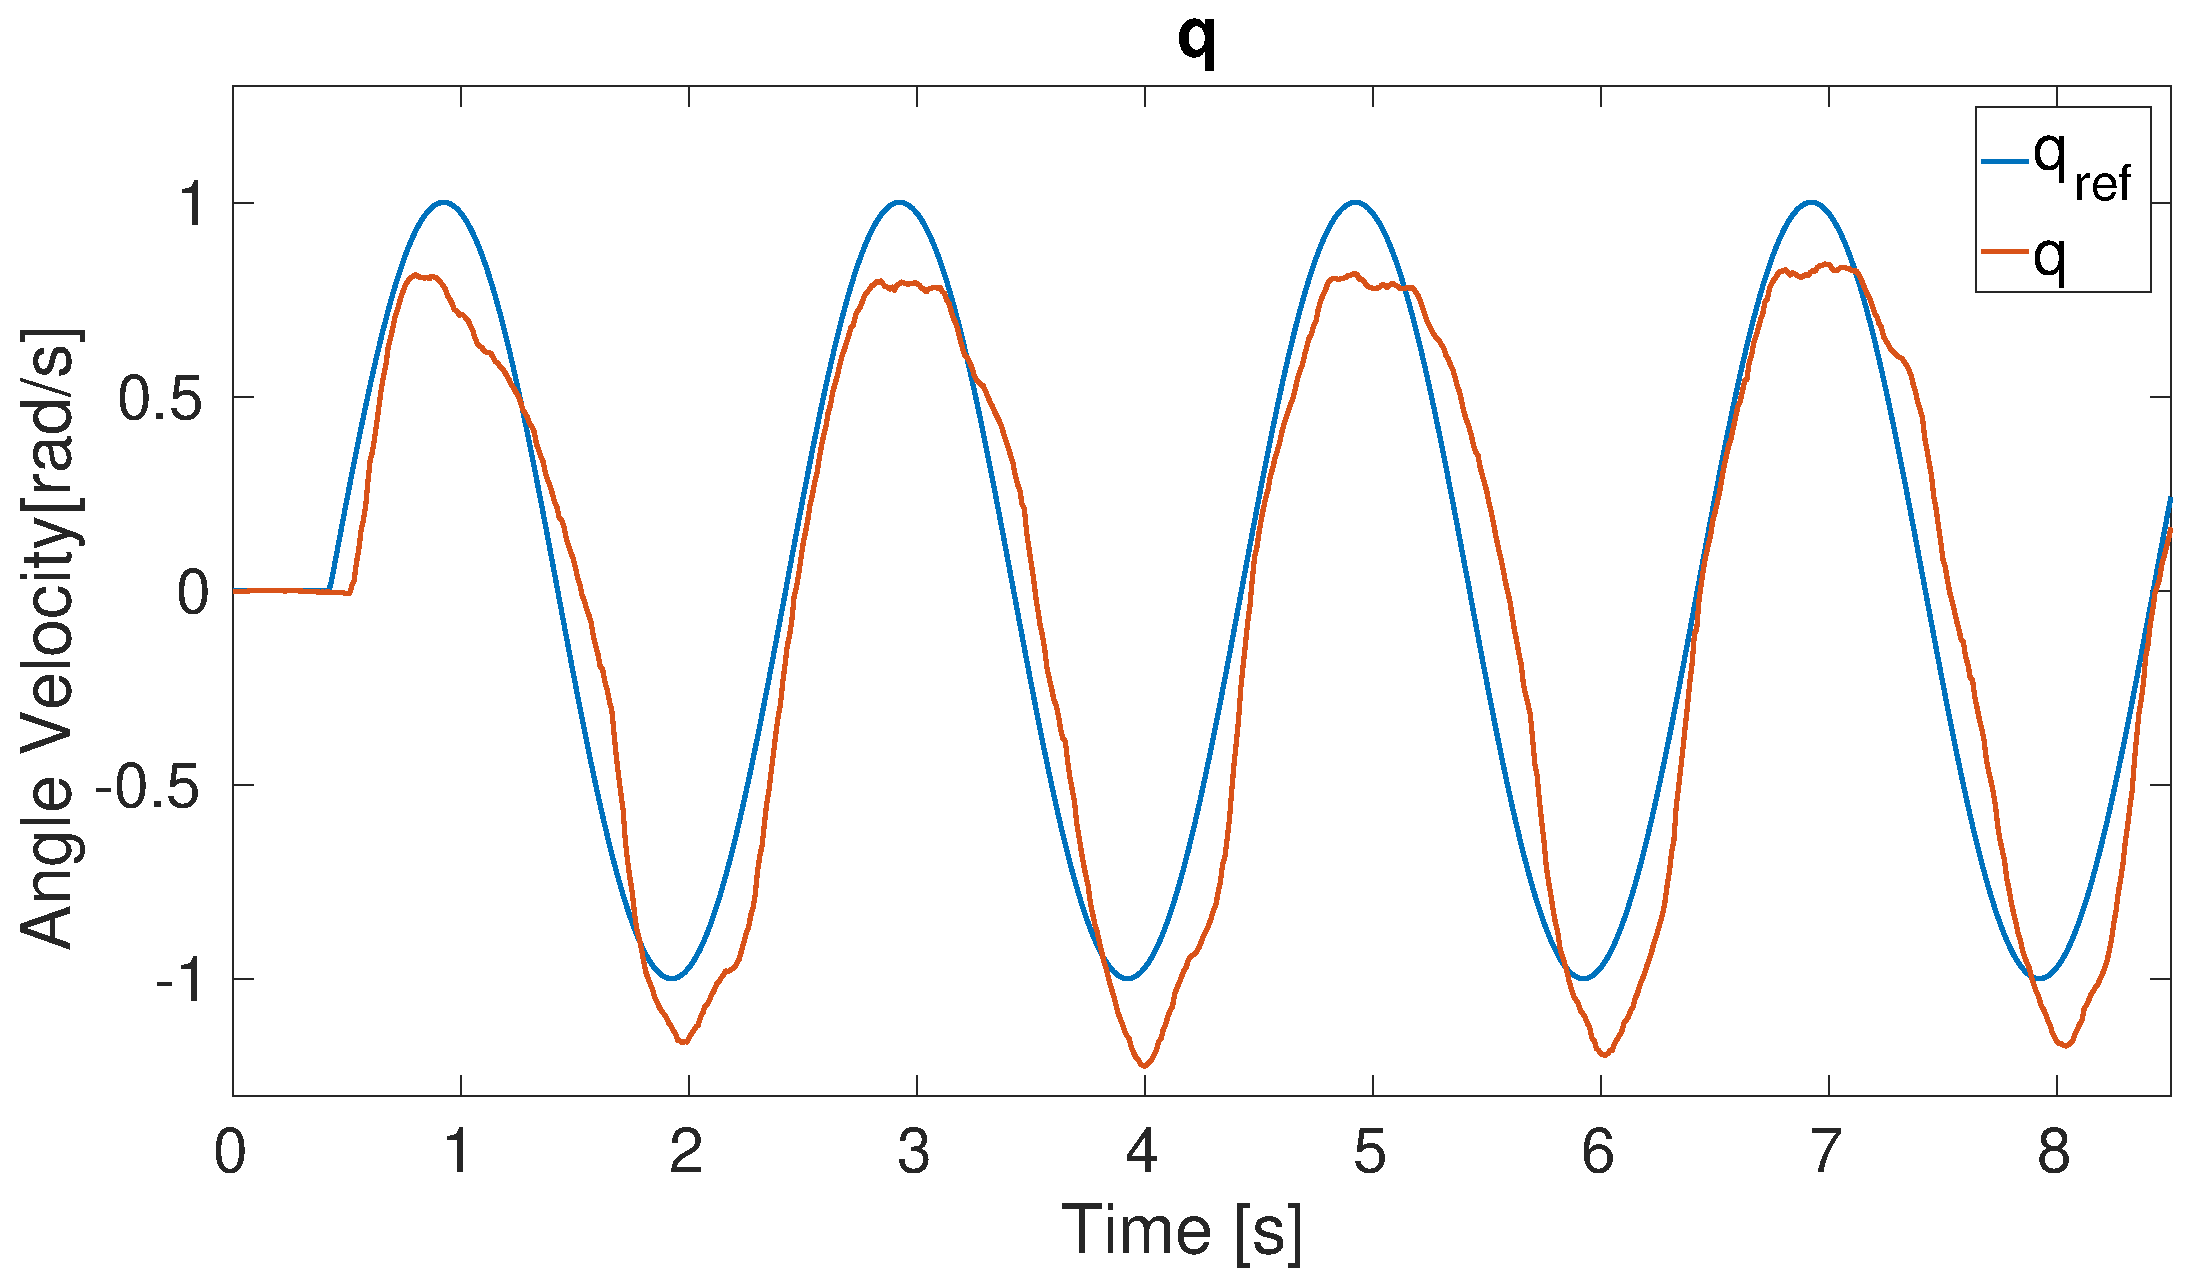
\includegraphics[width=0.4\textwidth]{testSinAllQA1}}
  \qquad
  \subfloat[][\label{fig:simSinAllQRate} A sine signal with amplitude $1$ and frequency $0.5\hertz$ applied to the simulated \abbrROV in $\pitchVelocity$.]{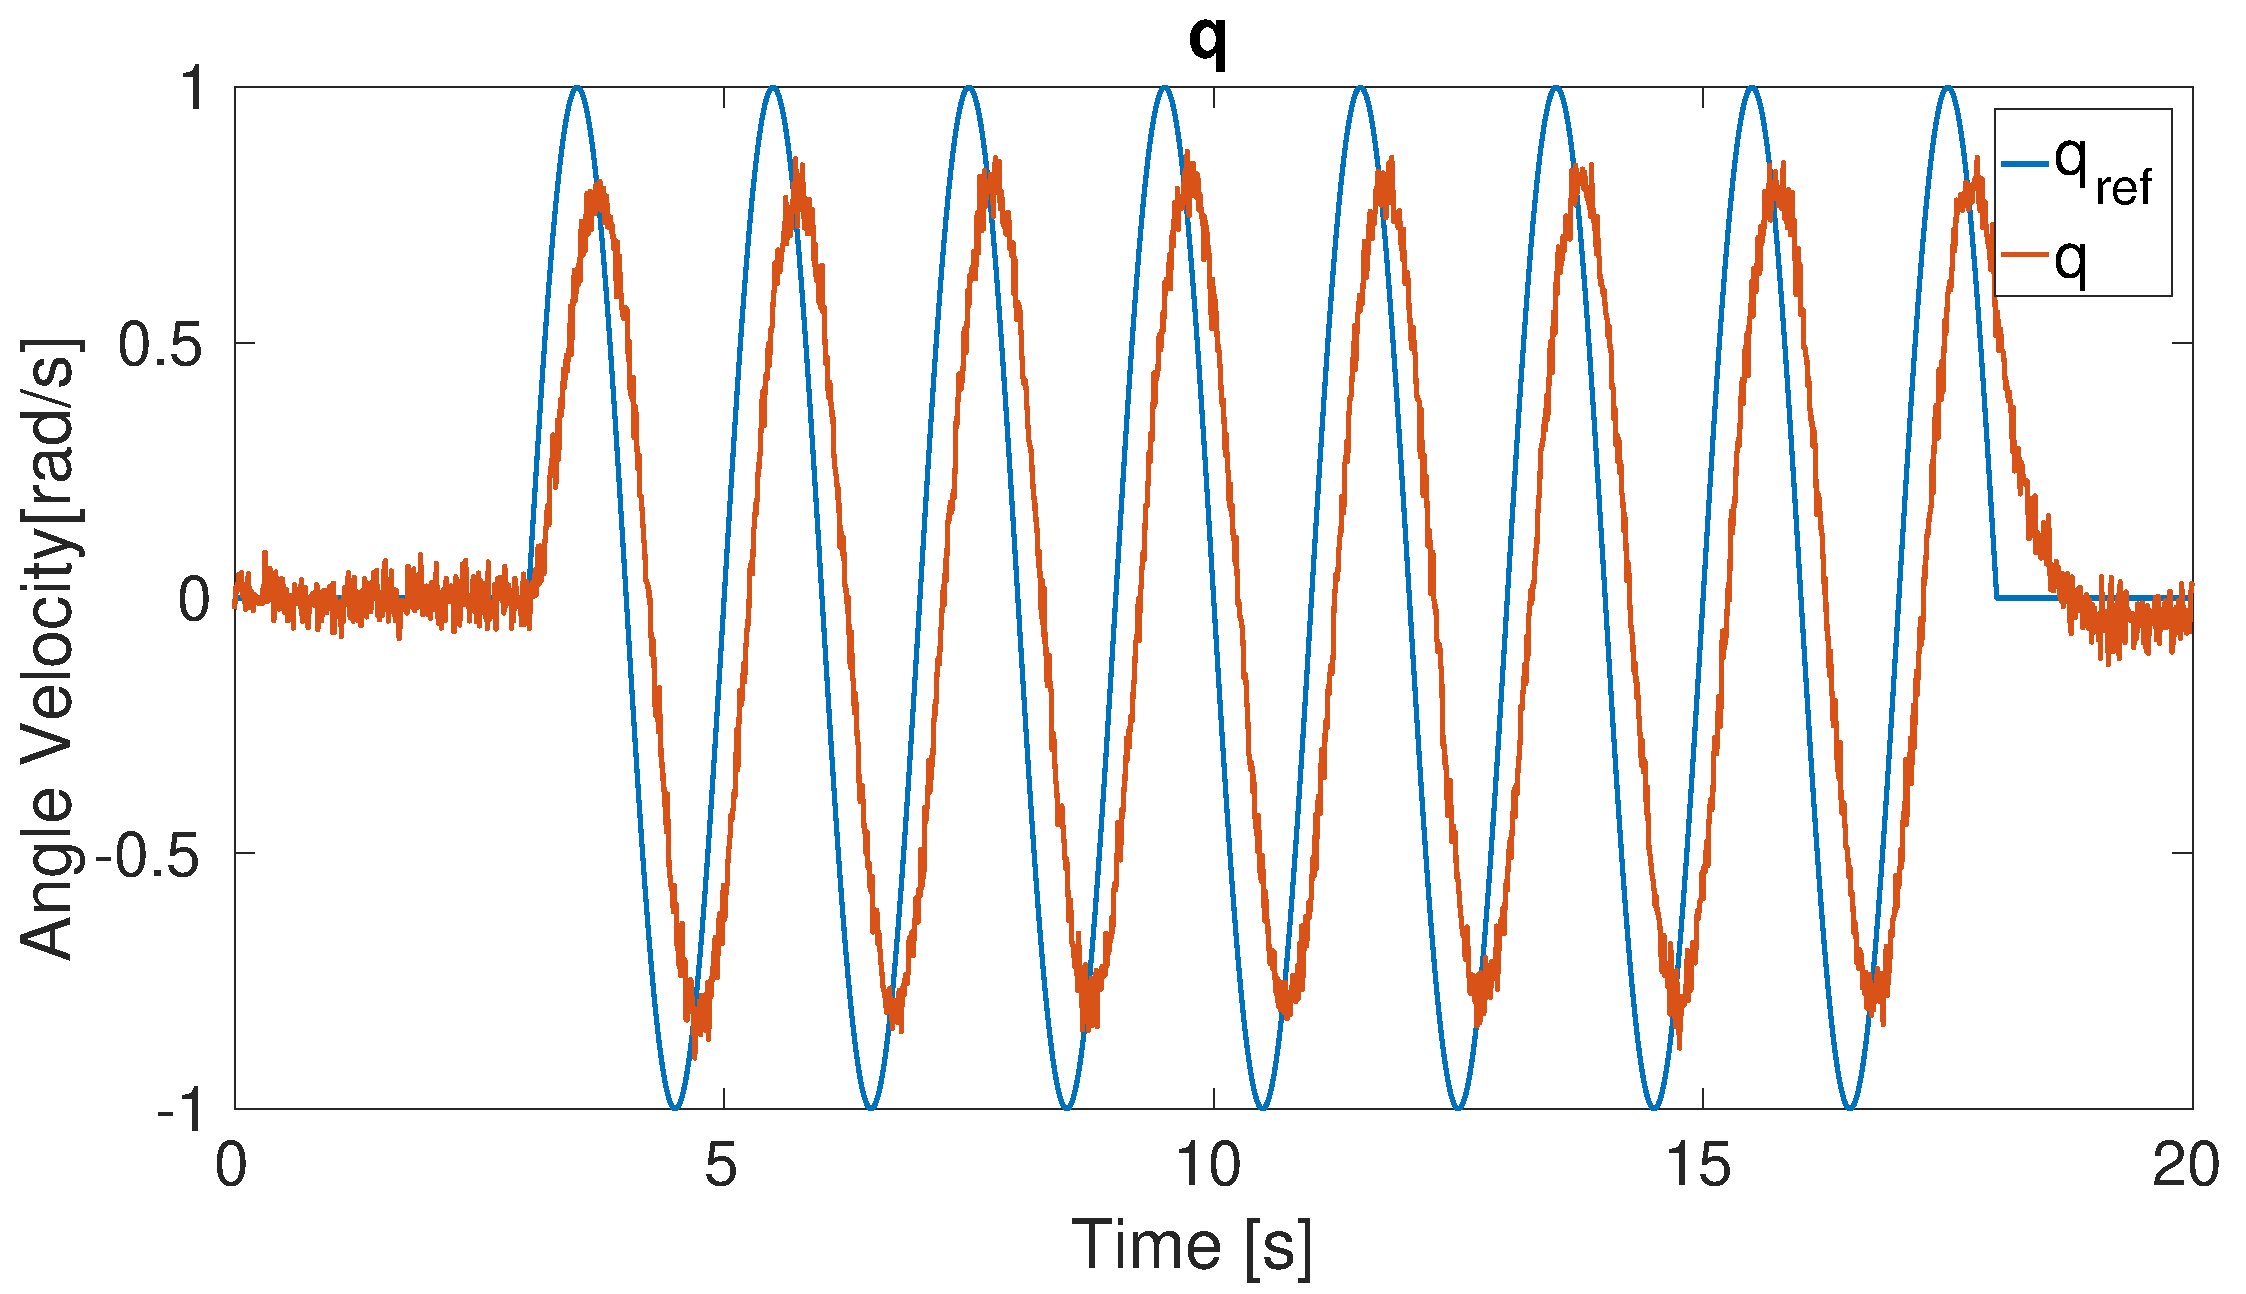
\includegraphics[width=0.4\textwidth]{simSinAllQA1}}
  \qquad
  \subfloat[][\label{fig:testSinAllRRate} A sine signal with amplitude $1$ and frequency $0.5\hertz$ applied in $\yawVelocity$.]{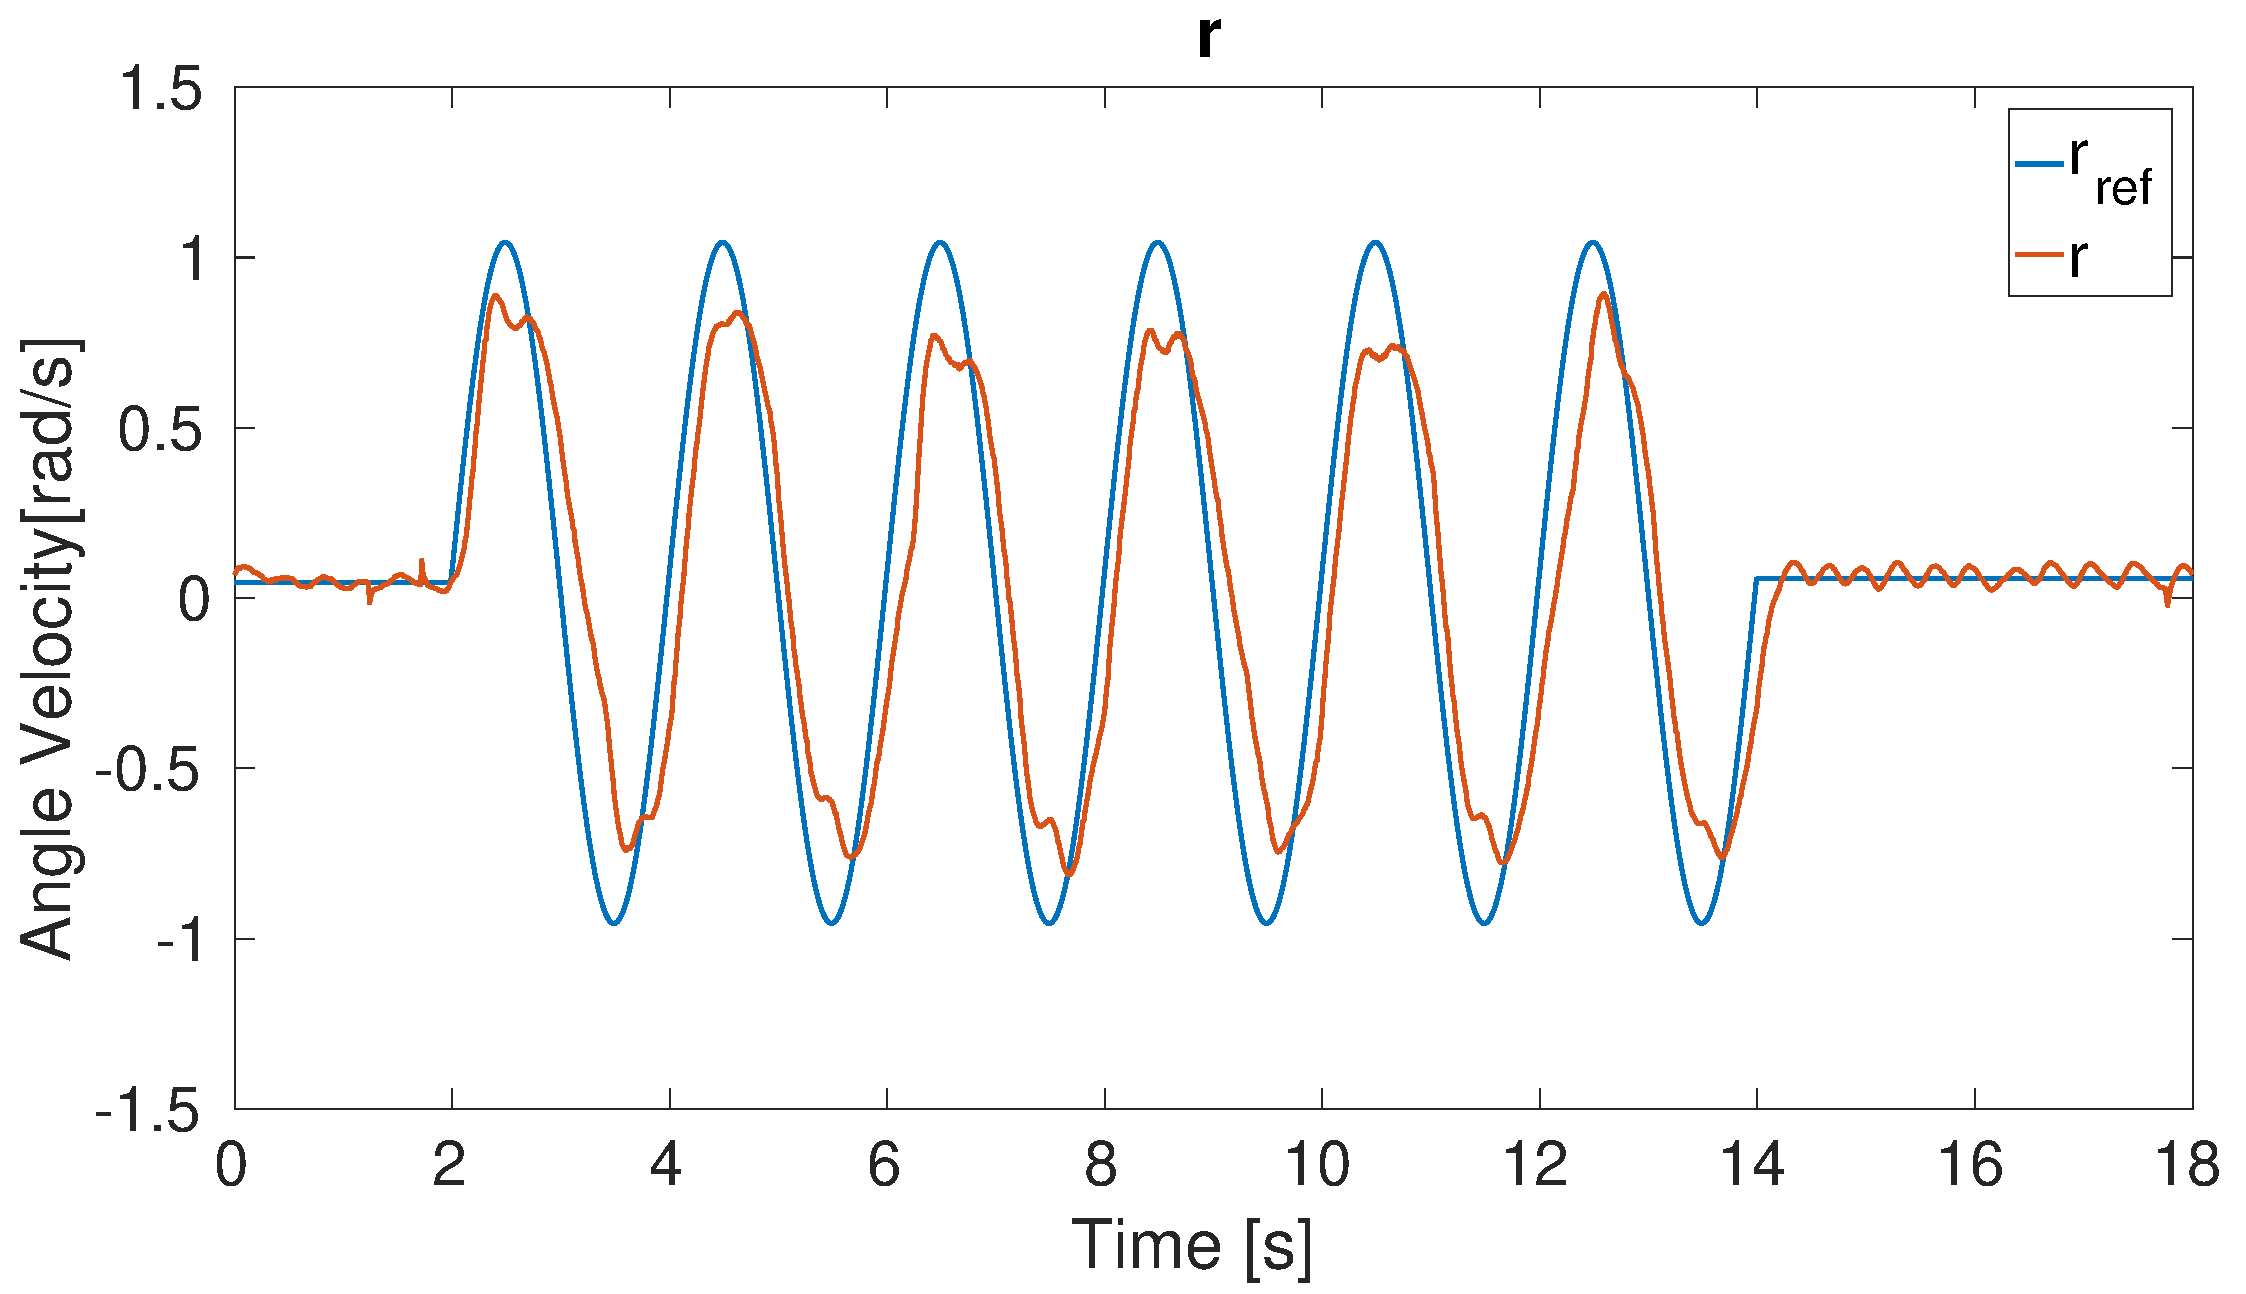
\includegraphics[width=0.4\textwidth]{testSinAllRA1}}
  \qquad
  \subfloat[][\label{fig:simSinAllRRate} A sine signal with amplitude $1$ and frequency $0.5\hertz$ applied to the simulated \abbrROV in $\yawVelocity$.]{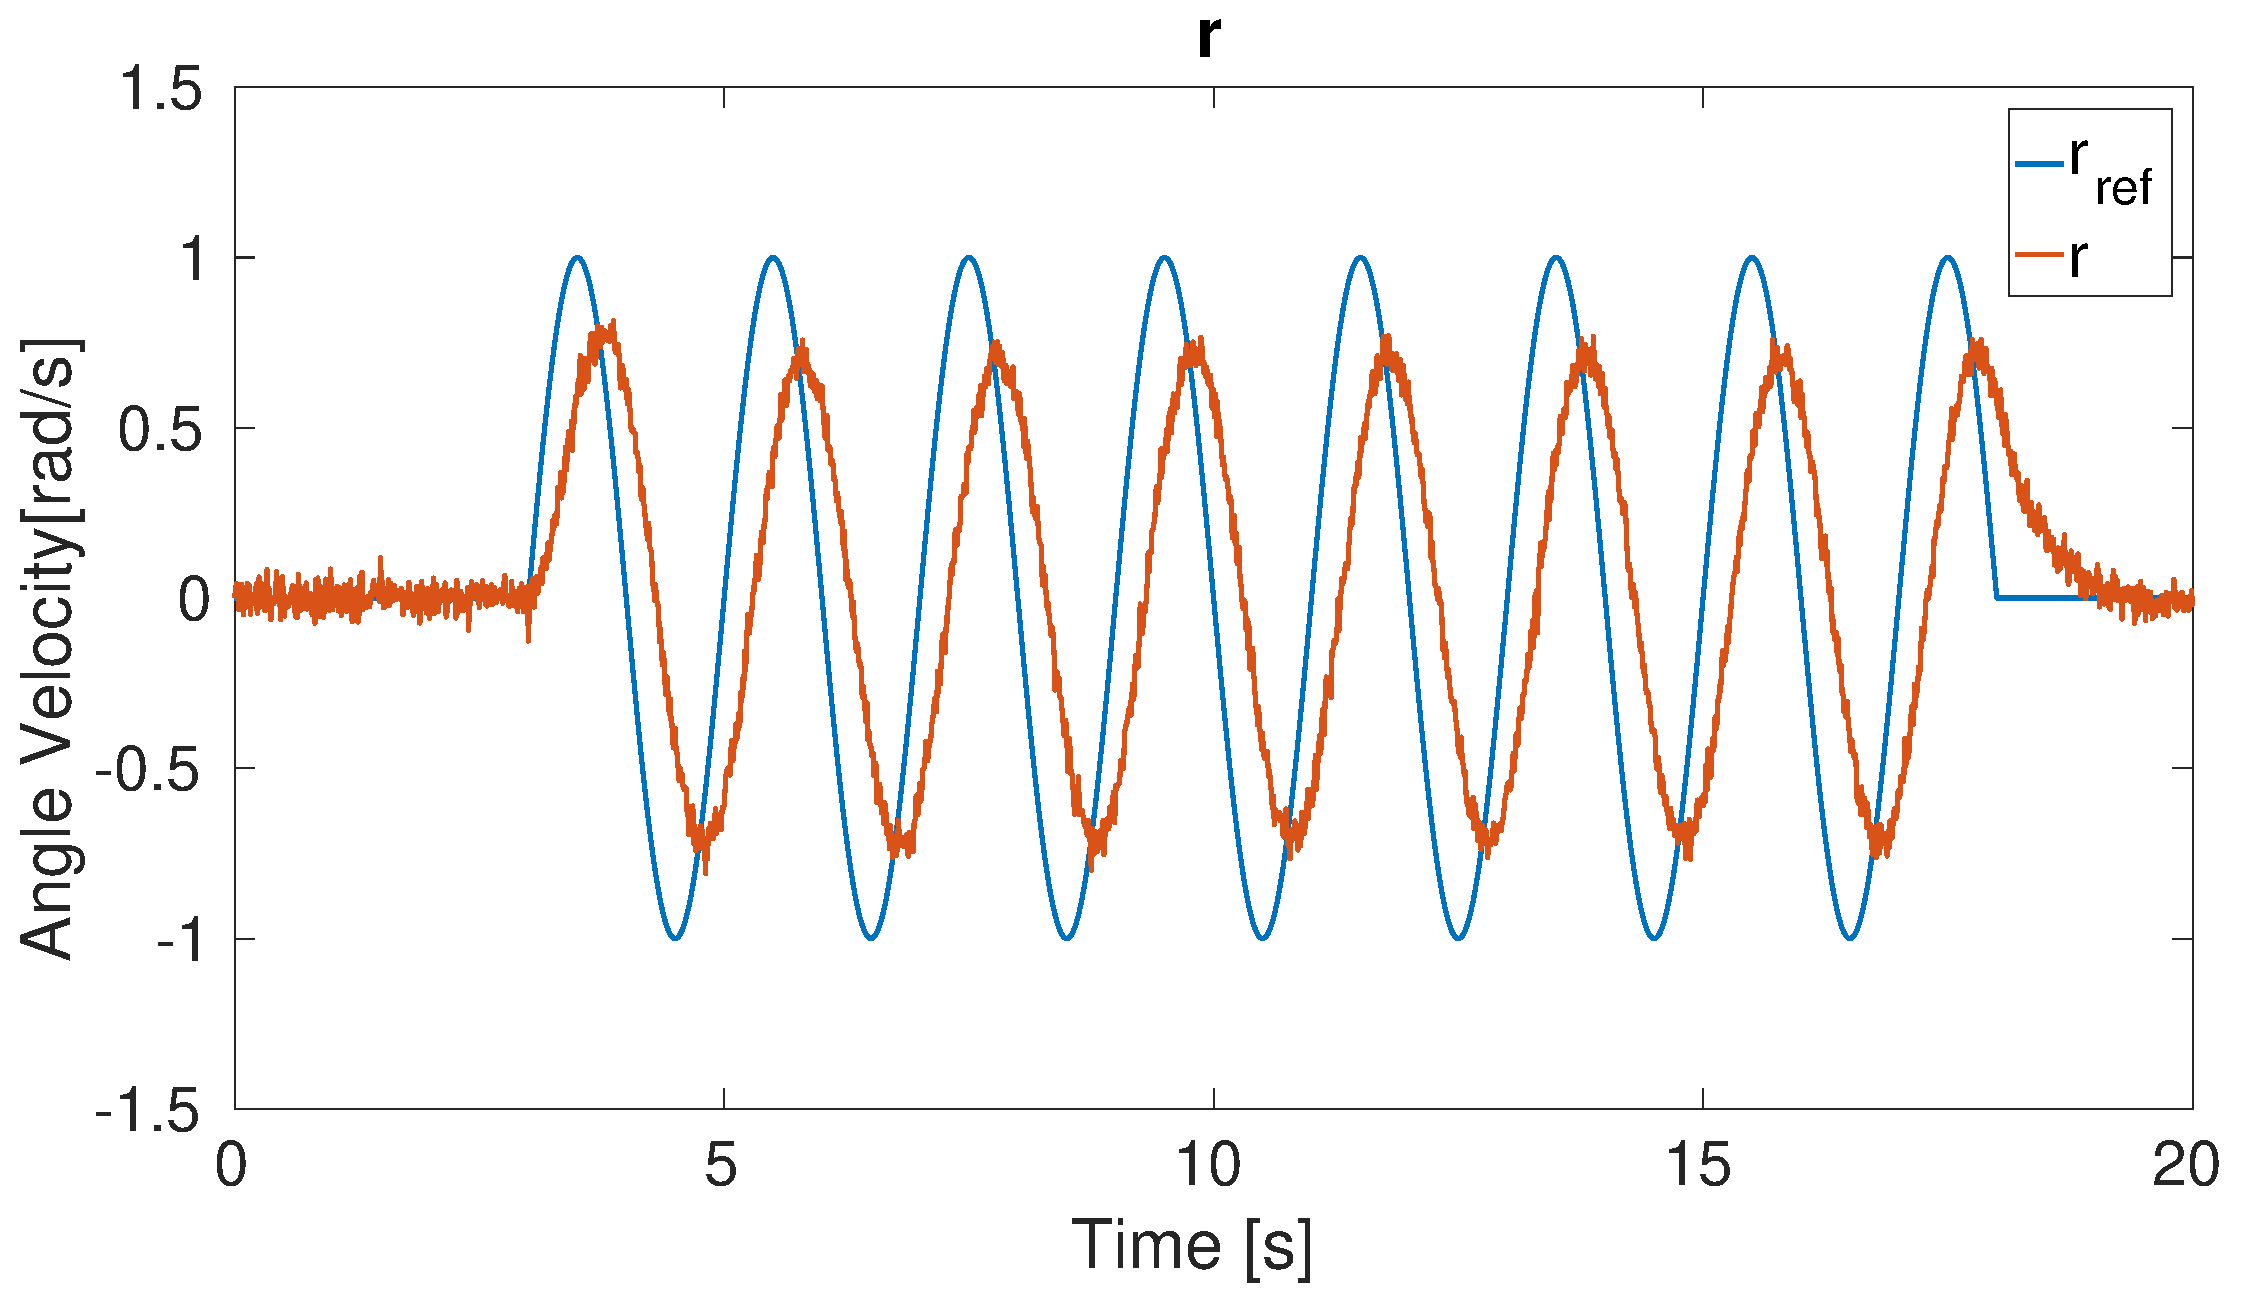
\includegraphics[width=0.4\textwidth]{simSinAllRA1}}
  \caption{\label{fig:SinAllRate}%
  Sine signals were applied in all angular velocities at the same time while using the rate controller.}
\end{figure}

Sine signals were applied to all angular velocities which can be seen in \Figureref{fig:SinAllRate} while using the rate controller. In the real test followed all the angular velocities the reference signals well, except for some overshoots and undershoots of the requested amplitude. The simulated test followed a general sine form but the reference amplitude was not reach and a phase shift could be noted.

%%%%%%%%%%%%%%%%%%%%%%%%%%%Depth%%%%%%%%%%%%%%%%
\begin{figure}[tbp]
  \centering
  \subfloat[][\label{fig:testStepD1} A smooth step applied in $\zPosition$.]{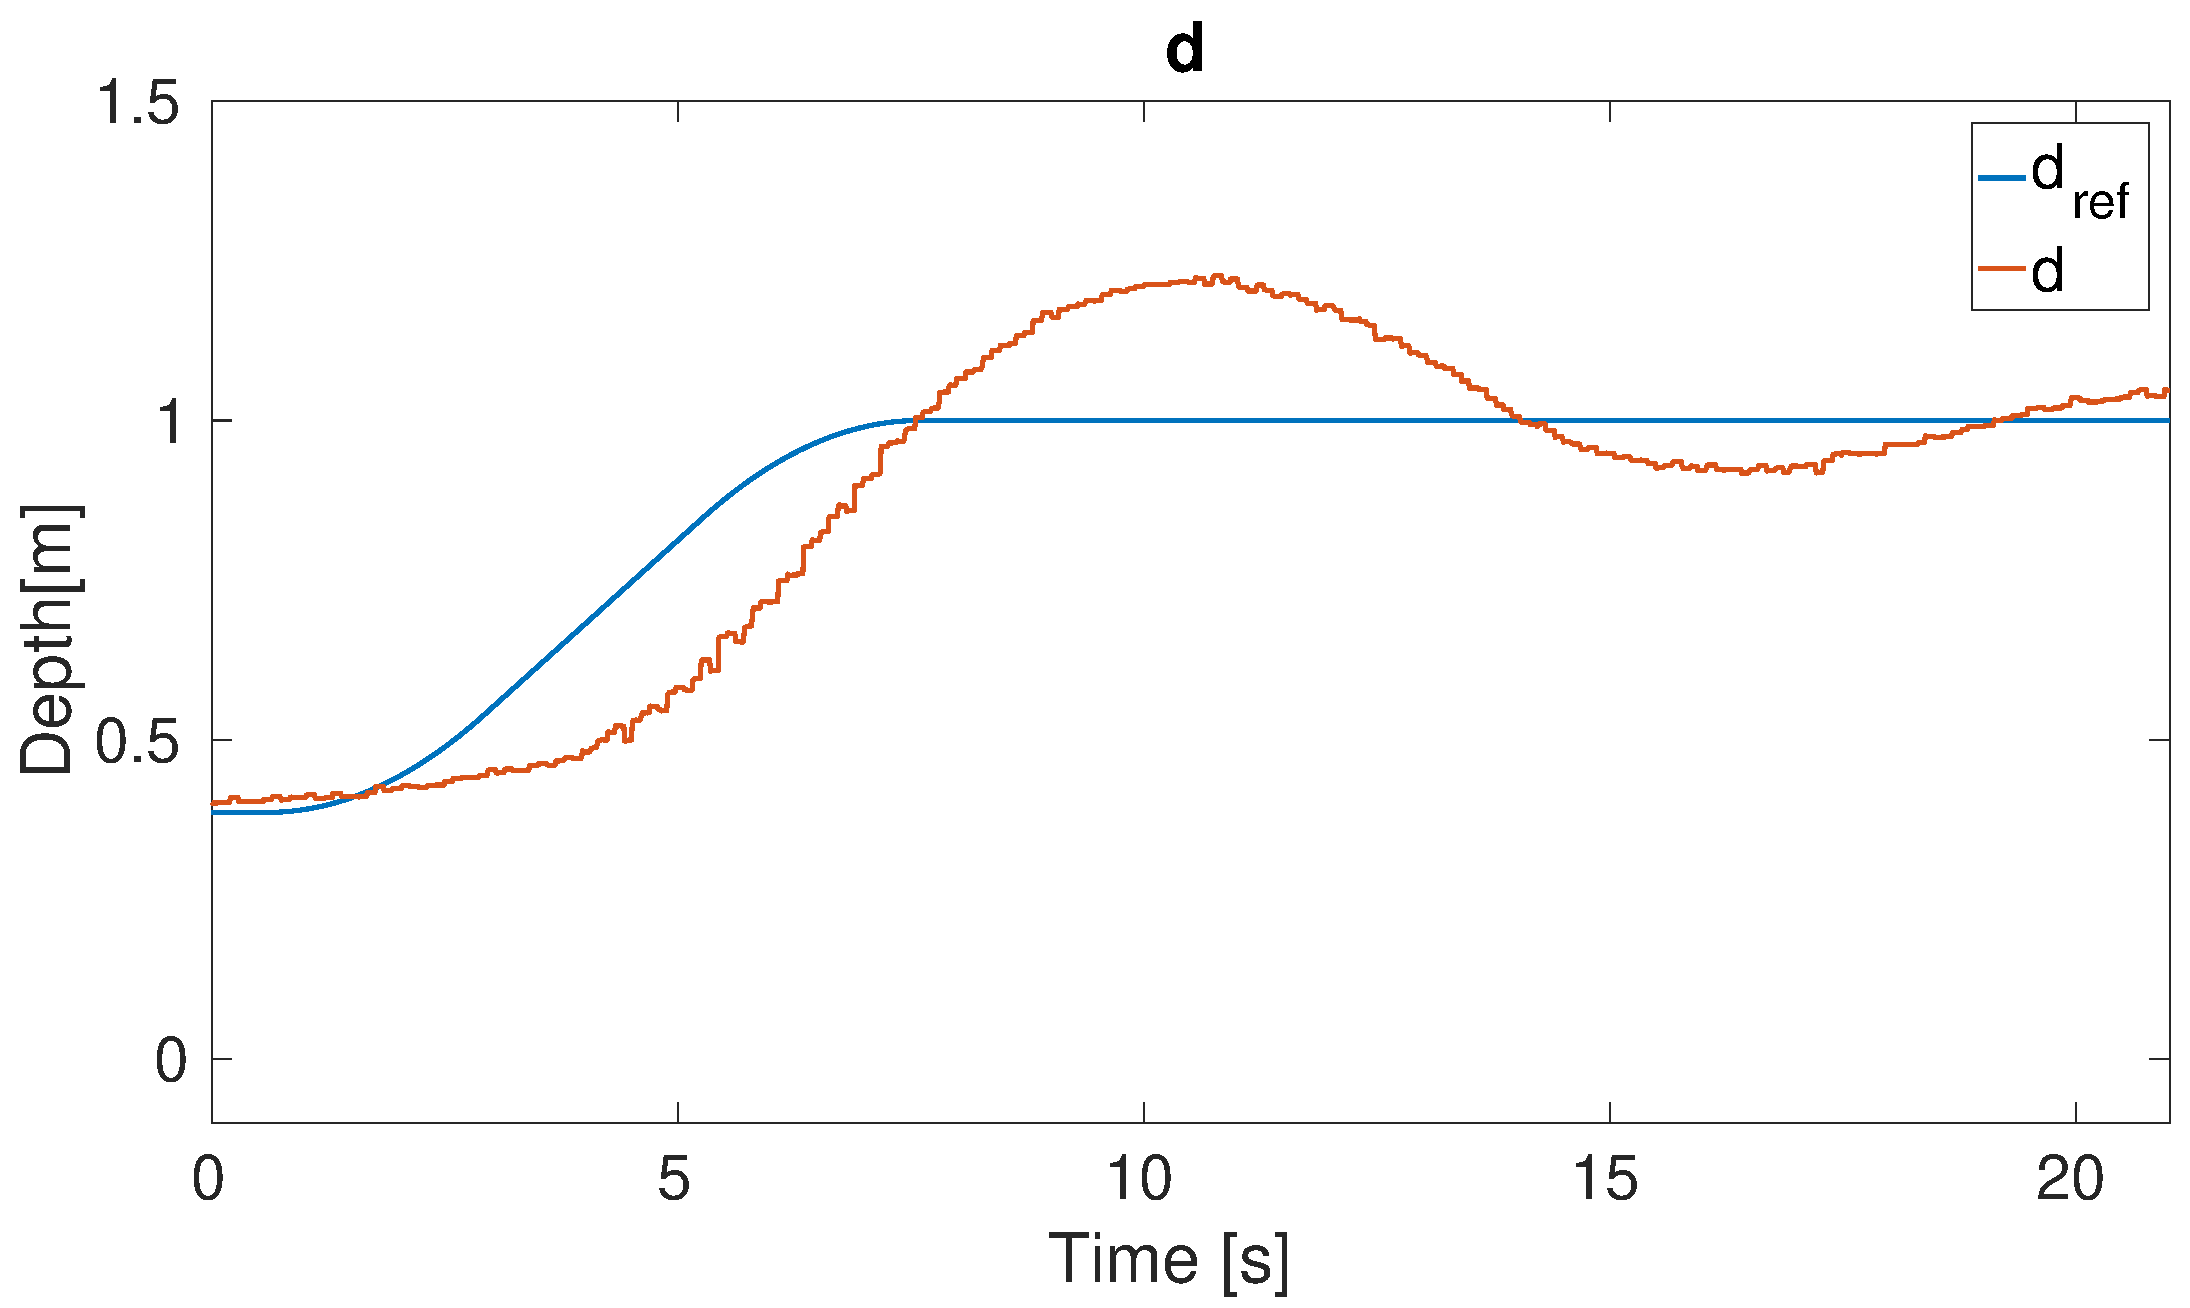
\includegraphics[width=0.4\textwidth]{testStepDepth3e10a1}}
  \qquad
  \subfloat[][\label{fig:testStepD2} A step applied in $\zPosition$.]{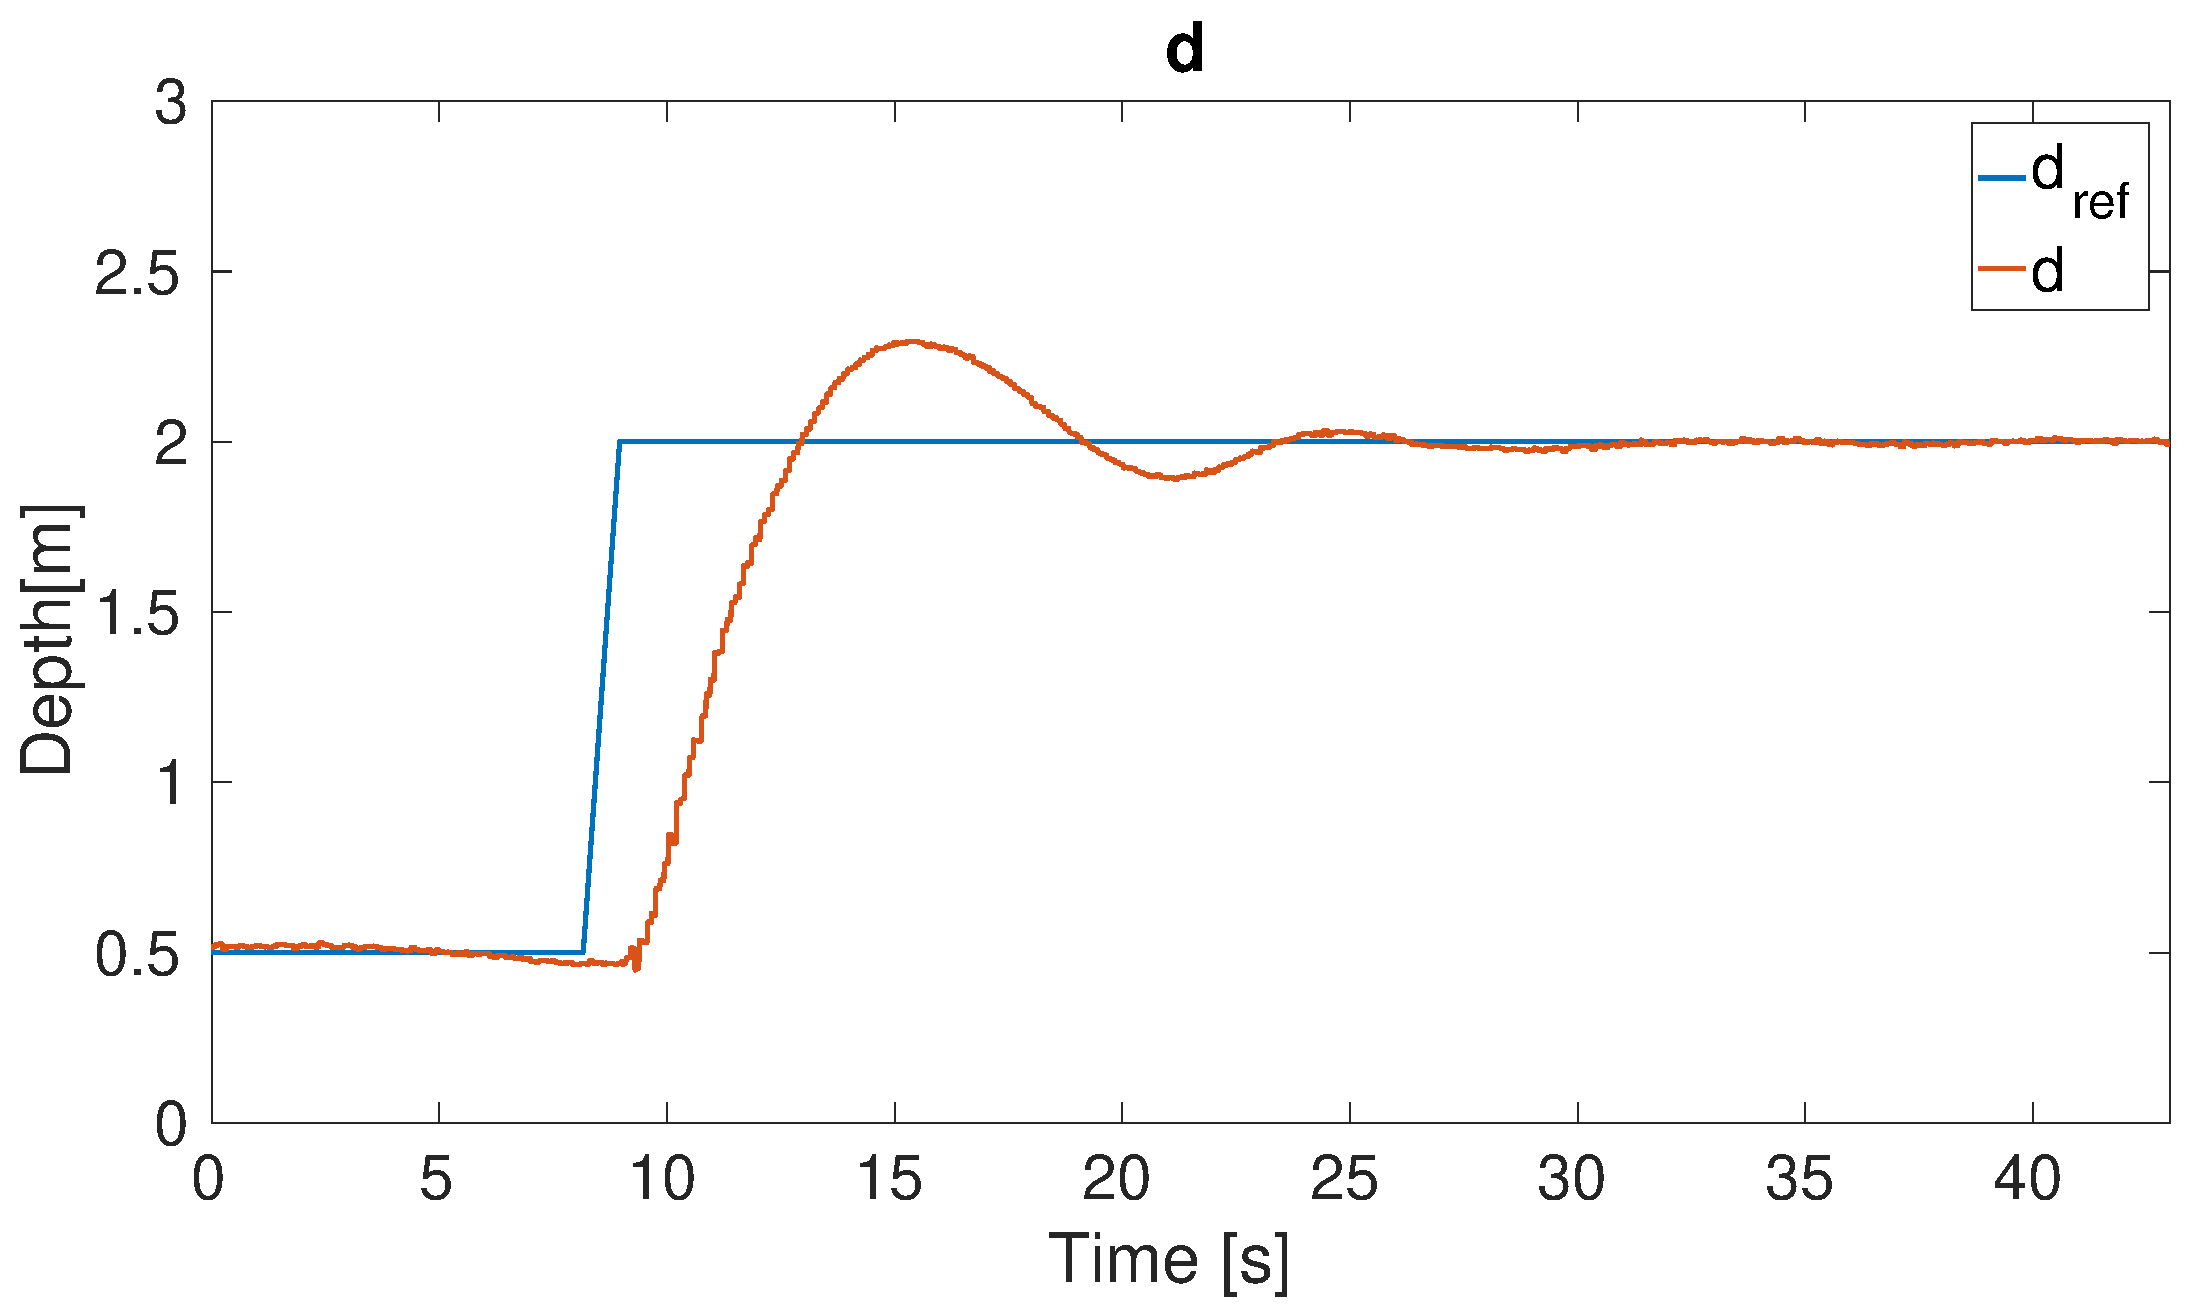
\includegraphics[width=0.4\textwidth]{testConstantD1}}
  \caption{\label{fig:StepD}%
    Steps applied to $\zPosition$. A smooth step from $0.4 \meter$ to $1 \meter$ is shown in (a) and a step from $0.5 \meter$ to $2 \meter$ is shown in (b).}
\end{figure}

\Figureref{fig:StepD} shows a smooth step from $0.4 \meter$ to $1 \meter$ and a step from $0.5 \meter$ to $2 \meter$. A delay in the response can be seen and overshoots of approximately 0.2.

%%%%%%%%%%%%%%%%%%%%%%%%%%%%%%%%%%%%%%%%
\section{Discussion}

